%%% On-going present
%%
%% Beginning of file 'sample.tex'
%%
%% Modified 2005 December 5
%%
%% This is a sample manuscript marked up using the
%% AASTeX v5.x LaTeX 2e macros.

%% The first piece of markup in an AASTeX v5.x document
%% is the \documentclass command. LaTeX will ignore
%% any data that comes before this command.

%% The command below calls the preprint style
%% which will produce a one-column, single-spaced document.
%% Examples of commands for other substyles follow. Use
%% whichever is most appropriate for your purposes.
%%
%%\documentclass[12pt,preprint]{aastex}

%% manuscript produces a one-column, double-spaced document:

%%\documentclass[manuscript]{aastex}

%% preprint2 produces a double-column, single-spaced document:

 %\documentclass[preprint2]{aastex}
%\documentclass[preprint2]{aastex}
%\documentclass[manuscript]{aastex}
\documentclass[iop]{emulateapj}
\renewcommand{\baselinestretch}{0.95}
%% Sometimes a paper's abstract is too long to fit on the
%% title page in preprint2 mode. When that is the case,
%% use the longabstract style option.

%% \documentclass[preprint2,longabstract]{aastex}

%% If you want to create your own macros, you can do so
%% using \newcommand. Your macros should appear before
%% the \begin{document} command.
%%
%% If you are submitting to a journal that translates manuscripts
%% into SGML, you need to follow certain guidelines when preparing
%% your macros. See the AASTeX v5.x Author Guide
%% for information.

\usepackage{enumitem} 

\newcommand{\hMsun}{{\ifmmode{h^{-1}{\rm
        {M_{\odot}}}}\else{$h^{-1}{\rm{M_{\odot}}}$~}\fi}} 
\newcommand{\hMpc}{{\ifmmode{h^{-1}{\rm Mpc}}\else{$h^{-1}$Mpc }\fi}}
\def\be{\begin{equation}}
\def\ee{\end{equation}}
\def\ba{\begin{eqnarray}}
\def\ea{\end{eqnarray}}


%% You can insert a short comment on the title page using the command below.

%\slugcomment{Not to appear in Nonlearned J., 45.}

%% If you wish, you may supply running head information, although
%% this information may be modified by the editorial offices.
%% The left head contains a list of authors,
%% usually a maximum of three (otherwise use et al.).  The right
%% head is a modified title of up to roughly 44 characters.
%% Running heads will not print in the manuscript style.

%\title[]
%{}

\shorttitle{Reshift Dependent Alcock-Paczynski effect from SDSS-III DR12}
\shortauthors{X.-D. Li, C. Park, C.G. Sabiu, H. Park, D.H. Weinberg, J. Kim, S.E. Hong}

%% This is the end of the preamble.  Indicate the beginning of the
%% paper itself with \begin{document}.

\begin{document}

%% LaTeX will automatically break titles if they run longer than
%% one line. However, you may use \\ to force a line break if
%% you desire.

\title{Cosmological constraints from the redshift dependence of the Alcock-Paczynski effect: application to the SDSS-III BOSS DR12 galaxies}


%\author{Xiao-Dong~Li\altaffilmark{1}, Changbom~Park\altaffilmark{1}, J.~E.~Forero-Romero\altaffilmark{2} and Juhan Kim%\altaffilmark{3}}
%\affil{\altaffilmark{1}School of Physics, Korea Institute for Advanced Study, Heogiro 85, Seoul 130-722, Korea }
%\affil{\altaffilmark{2}Departamento de F\'{i}sica, Universidad de los Andes, Cra. 1 No. 18A-10, Edificio Ip, Bogot\'a, %Colombia}
%\affil{\altaffilmark{3}Center for Advanced Computation, Korea Institute for Advanced Study, 85 Hoegi-ro, Dongdaemun-%gu, Seoul 130-722, Korea }
%\affil{\it (xiaodongli@kias.re.kr, cbp@kias.re.kr, je.forero@uniandes.edu.co, kjhan@kias.re.kr)}

%\author[Xiao-Dong~Li, Changbom~Park, Cristiano G. Sabiu, Juhan Kim and Sungwook E. Hong]
%{ Xiao-Dong Li$^{1,\dagger}$, Changbom Park$^{1}$, Cristiano G. Sabiu$^{2}$, Juhan Kim$^{3,1,\star}$, Sungwook E. Hong$^{1}$\\
%$^1$School of Physics, Korea Institute for Advanced Study, 85 Heogi-ro, Dongdaemun-gu, Seoul 130-722, Korea\\
%$^2$Korea Astronomy and Space Science Institute, 776, Daedeokdae-ro, Yuseong-gu, Daejeon, 305-348, Korea\\
%$^3$Center for Advanced Computation, Korea Institute for Advanced Study, 85 Hoegi-ro, Dongdaemun-gu, Seoul 130-722, Korea\\
%$^{\dagger}$xiaodongli@kias.re.kr\\
%$\star$Corresponding Author: ***@kasi.re.kr}

\author{Xiao-Dong Li, Changbom Park,}
\affil{School of Physics, Korea Institute for Advanced Study, 85 Heogiro, Dongdaemun-gu, Seoul 130-722, Korea}
\author{Cristiano G. Sabiu, Hyunbae Park,}
\affil{Korea Astronomy and Space Science Institute, Daejeon 305-348, Korea}
\author{David H. Weinberg,}
\affil{Department of Astronomy and CCAPP, The Ohio State University, 140 West 18th Avenue, Columbus, OH 43210, USA}
\author{Donald P. Schneider,}
\affil{Department of Astronomy and Astrophysics, The Pennsylvania State University, 
University Park, PA 16802 }
\affil{Institute for Gravitation and the Cosmos, The Pennsylvania State University, 
University Park, PA 16802 }
\author{Juhan Kim\altaffilmark{1},}
\affil{Center for Advanced Computation, Korea Institute for Advanced Study, 85 Hoegi-ro, Dongdaemun-gu, Seoul 130-722, Korea}
\affil{School of Physics, Korea Institute for Advanced Study, 85 Heogiro, Dongdaemun-gu, Seoul 130-722, Korea}
\and
\author{Sungwook E. Hong}
\affil{School of Physics, Korea Institute for Advanced Study, 85 Heogiro, Dongdaemun-gu, Seoul 130-722, Korea}

%\altaffiltext{1}{xiaodongli@kias.re.kr}
%\altaffiltext{2}{cbp@kias.re.kr}
%\altaffiltext{3}{csabiu@kasi.re.kr}
%\altaffiltext{4}{\bf Hyunbae: your email}
\altaffiltext{1}{Corresponding Author: kjhan@kias.re.kr}

% \email{xiaodongli@kias.re.kr}
% \email{cbp@kias.re.kr}
% \email{je.forero@uniandes.edu.co}



% \author{S. Djorgovski\altaffilmark{1,2,3} and Ivan R. King\altaffilmark{1}}
% \affil{Astronomy Department, University of California,
%     Berkeley, CA 94720}
%
% \author{C. D. Biemesderfer\altaffilmark{4,5}}
% \affil{National Optical Astronomy Observatories, Tucson, AZ 85719}
% \email{aastex-help@aas.org}
%
% \and
%
% \author{R. J. Hanisch\altaffilmark{5}}
% \affil{Space Telescope Science Institute, Baltimore, MD 21218}
%
% %% Notice that each of these authors has alternate affiliations, which
% %% are identified by the \altaffilmark after each name.  Specify alternate
% %% affiliation information with \altaffiltext, with one command per each
% %% affiliation.
%
% \altaffiltext{1}{Visiting Astronomer, Cerro Tololo Inter-American Observatory.
% CTIO is operated by AURA, Inc.\ under contract to the National Science
% Foundation.}
% \altaffiltext{2}{Society of Fellows, Harvard University.}
% \altaffiltext{3}{present address: Center for Astrophysics,
%     60 Garden Street, Cambridge, MA 02138}
% \altaffiltext{4}{Visiting Programmer, Space Telescope Science Institute}
% \altaffiltext{5}{Patron, Alonso's Bar and Grill}

%% Mark off your abstract in the ``abstract'' environment. In the manuscript
%% style, abstract will output a Received/Accepted line after the
%% title and affiliation information. No date will appear since the author
%% does not have this information. The dates will be filled in by the
%% editorial office after submission.

\begin{abstract}
We apply the methodology developed in \cite{Li2014,Li2015} to BOSS DR12 galaxies and 
derive cosmological constraints from the redshift dependence of the Alcock-Paczynski (AP) effect.
The apparent anisotropy in the distribution of observed galaxies arise from two main sources,
the redshift-space distortion (RSD) effect due to the galaxy peculiar velocities,
and the geometric distortion when incorrect cosmological models are assumed for 
%the coordinate transformation from redshift space to comoving space, 
transforming redshift to comoving distance,
known as the AP effect.
%We focus on the redshift dependence of the anisotropic clustering of galaxies to constrain cosmological parameters.
Anisotropies produced by the RSD effect are, although large,
maintaining a nearly uniform magnitude over a large range of redshift,
while the degree of anisotropies from the AP effect varies with redshift by much larger magnitude. 
%We found that the redshift dependence of the anisotropy introduced by RSD is much less significant compared with the anisotropy caused by AP.
%We focus on the redshift dependence of the anisotropic clustering of galaxies to constrain cosmological parameters 
%which is less sensitive to RSD contamination.
We split the DR12 galaxies into six redshift bins, measure the 2-point correlation function in each bin,
and assess the redshift evolution of anisotropies.
%Assuming a flat Universe consisting of a pressure-less dark matter component 
%with current ratio $\Omega_m$, and a dark energy component with constant equation of state $w$,
We obtain constraints of $\Omega_m=0.314 \pm 0.038,\ \ w = -1.09 \pm 0.14$,
which are tighter than the current constraints from other cosmological probes
such as type Ia supernovae, cosmic microwave background, and baryon acoustic oscillation (BAO).
Combining these cosmological probes with our method yield tight constraints of 
$\Omega_m = 0.304 \pm 0.007,\ w=-1.04 \pm 0.03$.
Our method is complementary to the other large scale structure probes like BAO and topology.
%We discuss the caveats and possibilities for improving upon our methodology.
We expect this technique will play an important role in deriving cosmological constraints from
large scale structure surveys.
\end{abstract}

%% Keywords should appear after the \end{abstract} command. The uncommented
%% example has been keyed in ApJ style. See the instructions to authors
%% for the journal to which you are submitting your paper to determine
%% what keyword punctuation is appropriate.

\keywords{large-scale structure of Universe --- dark energy --- cosmological parameters}

%% From the front matter, we move on to the body of the paper.
%% In the first two sections, notice the use of the natbib \citep
%% and \citet commands to identify citations.  The citations are
%% tied to the reference list via symbolic KEYs. The KEY corresponds
%% to the KEY in the \bibitem in the reference list below. We have
%% chosen the first three characters of the first author's name plus
%% the last two numeral of the year of publication as our KEY for
%% each reference.


%% Authors who wish to have the most important objects in their paper
%% linked in the electronic edition to a data center may do so by tagging
%% their objects with \objectname{} or \object{}.  Each macro takes the
%% object name as its required argument. The optional, square-bracket
%% argument should be used in cases where the data center identification
%% differs from what is to be printed in the paper.  The text appearing
%% in curly braces is what will appear in print in the published paper.
%% If the object name is recognized by the data centers, it will be linked
%% in the electronic edition to the object data available at the data centers
%%
%% Note that for sources with brackets in their names, e.g. [WEG2004] 14h-090,
%% the brackets must be escaped with backslashes when used in the first
%% square-bracket argument, for instance, \object[\[WEG2004\] 14h-090]{90}).
%%  Otherwise, LaTeX will issue an error.

\section{Introduction}

The current standard model of cosmology has been highly successful at reproducing the Universe on large scales. %large scale observations of the Universe. 
From the temperature fluctuations in the cosmic microwave background (CMB), 
to the late time clustering of galaxies, 
the vacuum energy dominated cold dark matter model ($\Lambda$CDM) fits the data surprisingly well \citep{Planck2015,Anderson2013}. 
This result is all the more impressive considering both the underlying assumptions, 
such as homogeneity, isotropy, scale invariance of the primordial fluctuations, 
and the minimal set of cosmological parameters that are required.

Nonetheless, these models produce the unsatisfactory prospect that we must include within our ontology both a vacuum energy 
that is much smaller than that predicted from  quantum mechanics, 
or alternatively a new scalar field (dark energy) that has negative pressure
\citep{SW1989,Riess1998,Perl1999,PR2003,Li2011}, 
and a new matter component, which is not contained within the standard $SU(3)\times SU(2) \times U(1)$ formulation of particle physics.


With an over-abundance of models for both dark energy-like accelerated expansion and dark matter, 
it is crucial to obtain precise and model-independent measurements of the cosmic evolution, usually referred to as background observables. 
Two such observables are the angular diameter distance, $D_A$, and the Hubble factor, $H$.  
If these quantities can be measured at various redshifts and to a high degree of accuracy then our ability to differentiate between various competing models will be greatly increased.

In the last few years there has been increasing interest in using the Alcock-Paczynski (AP) effect \citep{AP1979} 
in the large-scale clustering of galaxies to obtain constraints on $D_A$ and $H$ \citep{Guzzo2008,topology}. 
Assuming an incorrect cosmological model for the coordinate transformation from redshift space to comoving space produces residual geometric distortions. 
These distortions are induced by the fact that measured distances along and perpendicular to the line of sight are fundamentally different. 
Measuring the ratio of galaxy clustering in the radial and transverse directions provides a probe of this AP effect.

There have been several methods proposed for applying the AP test to the large scale structure (LSS).
The most widely adopted one uses anisotropic clustering \citep{Ballinger1996,Matsubara1996},
which has been used for the 2 degree Field Quasar Survey \citep{Outram2004},
the WiggleZ dark energy survey \citep{Blake2011}, 
the Sloan Digital Sky Survey-I/II (SDSS-I/II) Luminous Red Galaxy (LRG) survey \citep{Eisenstein et al. 2011,ChuangWang2012},
and the SDSS-III Baryon Oscillation Spectroscopic Survey (BOSS) 
%\citep{Reid2012,Beutler2013,Linder2013,2014arXiv1407.2257S, 2014ApJ...781...96L}.
\citep{Reid2012,Beutler2013,Linder2013,2014arXiv1407.2257S, 2014ApJ...781...96L,
Alam2016, Beutler2016, Sanchez2016}
The main caveat of this method is that,
because the radial distances of galaxies are inferred from redshifts,
AP tests are inevitably limited by redshift-space distortions (RSD) \citep{Ballinger1996},
which leads to apparent anisotropy even if the adopted cosmology is correct.
The RSDs must be accurately modeled for the 2-point statistics of galaxy clustering.


\cite{Marinoni2010} proposed using the symmetry properties of galaxy pairs.
Unfortunately this method is also seriously limited by RSD.
The peculiar velocity distorts the redshift and changes the apparent tilt angles of galaxy pairs.
The effect depends on both redshift and underlying cosmology, and is rather difficult to model accurately \citep{Jennings2011}.
\cite{Ryden1995} and \cite{LavausWandelt1995} proposed another method using the apparent stretching of voids.
This approach has the advantage that the void regions are easier to model compared with dense regions,
but has limitations in that it utilizes only low density regions of the LSS
and requires large samples.

\cite{Li2014} proposed another method utilizing the redshift dependence of AP effect to overcome the RSD problem.
The anisotropies produced by RSD effect are, although very large,
close to uniform in magnitude over a large range of redshift.
Conversely, if cosmological parameters are incorrectly chosen, the LSS
appear anisotropic and the degree of anisotropy varies with redshift. 
%We found that the redshift dependence of the anisotropy introduced by RSD is much less significant compared with the anisotropy caused by AP.
%Thus we can focus on the redshift dependence of the galaxy density gradient field, 
%which is less affected by RSD, but still sensitive to cosmological parameters.
We used the {\it galaxy density gradient field} 
to characterize the anisotropies in LSS and tested the idea on Horizon Run 3 (HR3) N-body simulations \citep{horizonrun},
demonstrating that the method leads to unbiased estimation of the density parameter $\Omega_m$ and the dark energy equation of state (EoS) $w$.

The same topic was revisited in \cite{Li2015}, but using the {\it galaxy two-point correlation function} (2pCF) as the statistical tool.
The 2pCF as a function of angle, $\xi(\mu)$, is measured at different redshifts.
Similar to \cite{Li2014}, we found that the RSD effect, although significantly distorting $\xi(\mu)$, 
exhibits much less redshift evolution compared to the amount of change in $\xi(\mu)$ due to incorrectly adopted cosmologies.
When incorrect cosmological parameters are adopted, 
the shape of $\xi(\mu)$ appears anisotropic due to the AP effect, 
and the amplitude is shifted by the change in comoving volume;
both effects have significant redshift dependence.
%By focusing on the redshift dependence of $\xi(\mu)$, we can correctly recover the cosmological parameters despite the contamination of RSD.
We test the method using the 2pCF on mock surveys drawn from HR3
%we measuring the redshift evolution of 2pCF also leads to unbiased estimation of cosmological parameters 
and find the constraints obtained are tighter than those from the methodology of \cite{Li2014}.

The change of the comoving volume size is another consequence of an incorrectly adopted cosmology, 
and has motivated investigations constraining cosmological parameters from number counting of 
galaxy clusters \citep{PS1974,VL1996}. 
An obstacle in using the comoving volume for cosmological tests is the evolution of the number of target objects.
The essential need for reducing the evolution effects in applying the test led \cite{topology} to propose a new method
using the topology of LSS. 
Since the topology is a measure of intrinsic connectivity of structures,
it is expected to be insensitive to non-linear gravitational evolution, type of density tracers,
and RSD on large scales.
This method has been applied to the WiggleZ Dark Energy Survey data by \cite{WiggleZtopoloy},
and to simulated BOSS samples \citep{Speare2015}.


In this paper we apply our methodology to SDSS-III BOSS Data Release 12 (DR12) galaxies \citep{Reidetal:2016}.
%We split the DR12 samples of CMASS and LOWZ into six redshift bins (three in each) and measure the redshift evolution of 
%anisotropy therein to determine the correct cosmological parameters leading to least redshift evolution of anisotropy.
We take the 2pCF as statistical tool characterizing the anisotropic clustering and follow the procedure of \cite{Li2015} to conduct the analysis.
We assume a flat Universe and constrain parameters of $\Omega_m$ and $w$.
2pCF is a mature statistic in cosmology and its optimal estimation and statistical properties are well understood.
Compared with the density gradient field statistic, it leads to tighter constraints and is less affected by survey geometry.


The outline of this paper is as follows. 
In Sec. 2 we describe the observational data used in this paper.
In Sec. 3 we discuss the N-body simulations and mock galaxy catalogues that are used in this analysis.
In Sec. 4 we briefly review the nature and consequences of the AP effect when performing coordinate transforms in a cosmological context. 
In Sec. 5 and Sec. 6, we describe our analysis method and present the cosmological constraints obtained from BOSS DR12 galaxies. 
We conclude in Sec. 7.

%{\bf AMTB: Please chose one kind of tense of verbs. It changes from sentences to sentences!}
%{\bf AMTB: How many mock BOSS samples are made from HR4?}



\section{The Observational Data}\label{sec:data}

The Sloan Digital Sky Survey (SDSS; York et al. 2000) %DANGEROUS
imaged approximately 7\,606 $\rm deg^2$
of the Northern Galactic Hemisphere and 
3\,172 $\rm deg^2$ of the Southern Galactic Hemisphere in the {\it ugriz} bands \citep{Fukugita1996,Gunn1998}.
The survey was performed using the 
2.5m Sloan telescope \citep{Gunn et al. 2006}
at the Apache Point Observatory in New Mexico.
%BOSS, as part of the SDSS-III survey \citep{Eisenstein et al. 2011},
%has obtained additional imaging,
%increasing the region of the south to 3\,172 $\rm deg^2$.
BOSS \citep{Dawson et al. 2012,Smee2013}, as a part of the SDSS-III survey \citep{Eisenstein et al. 2011},
has obtained spectra and redshifts 
of 1.37 million galaxies selected from the SDSS imaging,
covering a region of 9\,376 $\rm deg^2$.
The galaxy redshifts were measured by an automated pipeline \citep{Bolton2012}.

\begin{figure*}
   \centering{
   %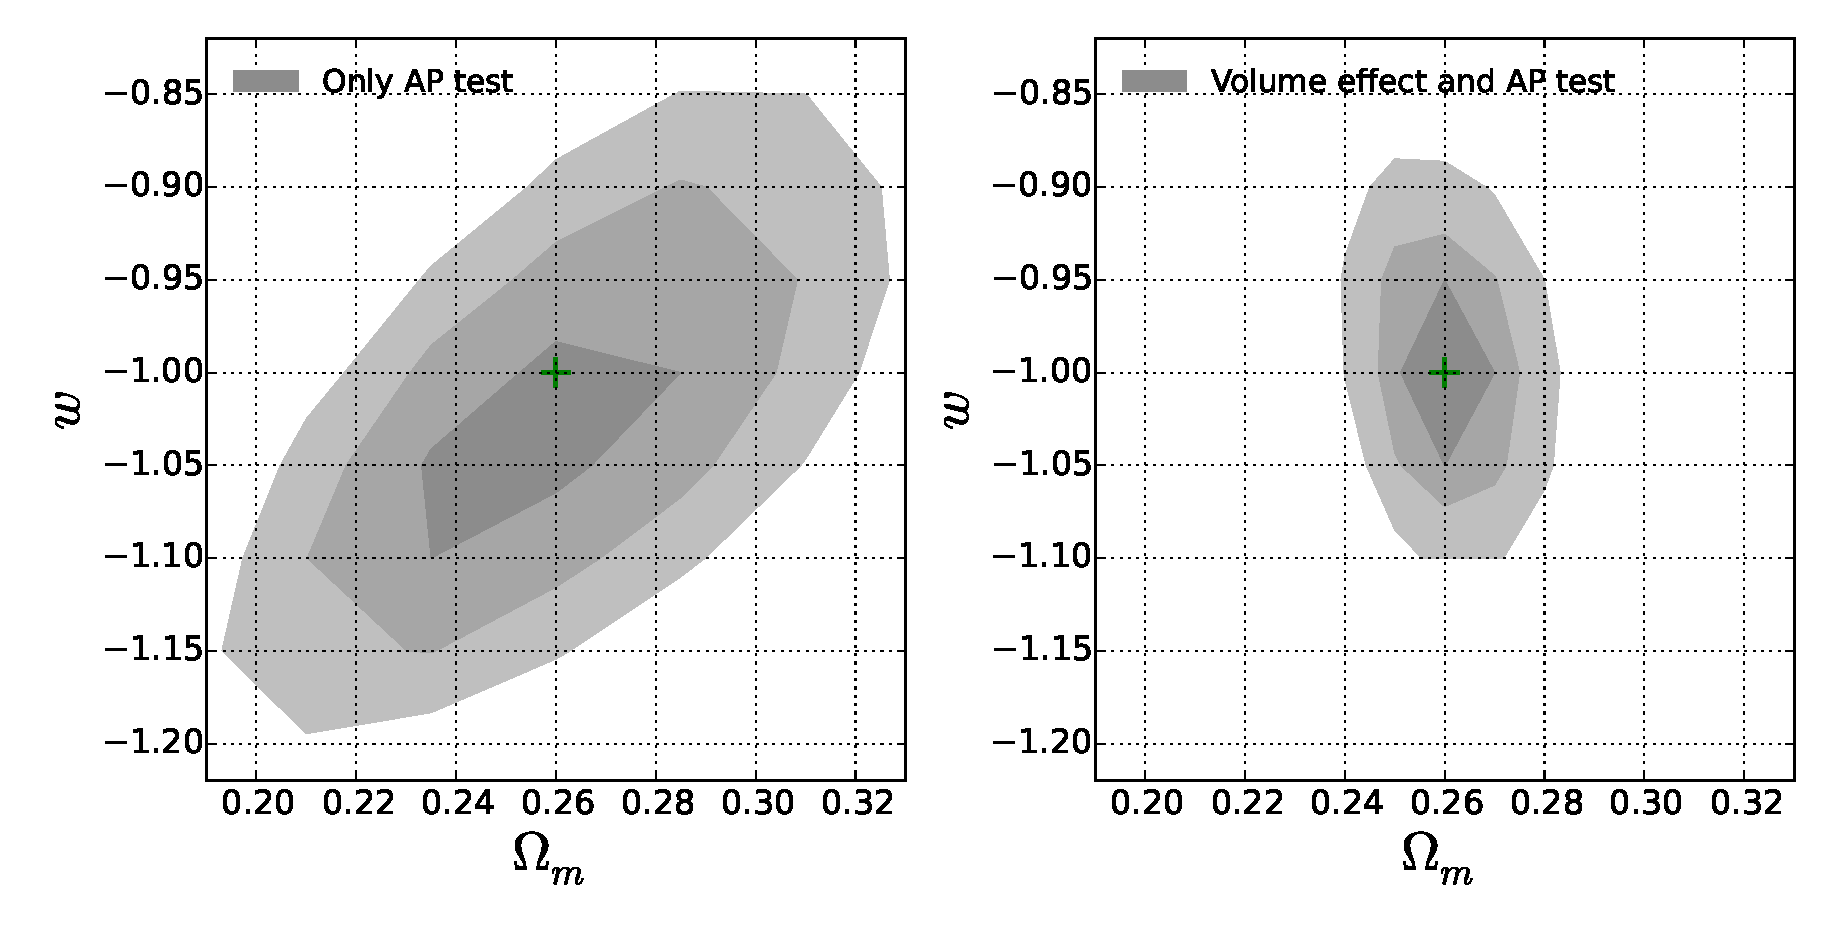
\includegraphics[width=7cm]{Tpcf--contour.eps}
   %\includegraphics[width=16cm]{Tpcf--contour-others.eps}
   %\includegraphics[width=7.5cm,natwidth=8.3,natheight=9]{maskdr12v1lowres.png}
   %\includegraphics[width=7.5cm,natwidth=8.3,natheight=9]{maskdr12v1lowzlowres.png}
   %\includegraphics[width=8.5cm,natwidth=8.3,natheight=5]{Tpcf--gal_LN.jpg}
   %\includegraphics[width=8.5cm,natwidth=8.3,natheight=5]{Tpcf--gal_LS.jpg}
   %\includegraphics[width=8.5cm,natwidth=8.3,natheight=5]{Tpcf--gal_CN.jpg}
   %\includegraphics[width=8.5cm,natwidth=8.3,natheight=5]{Tpcf--gal_CS.jpg}
   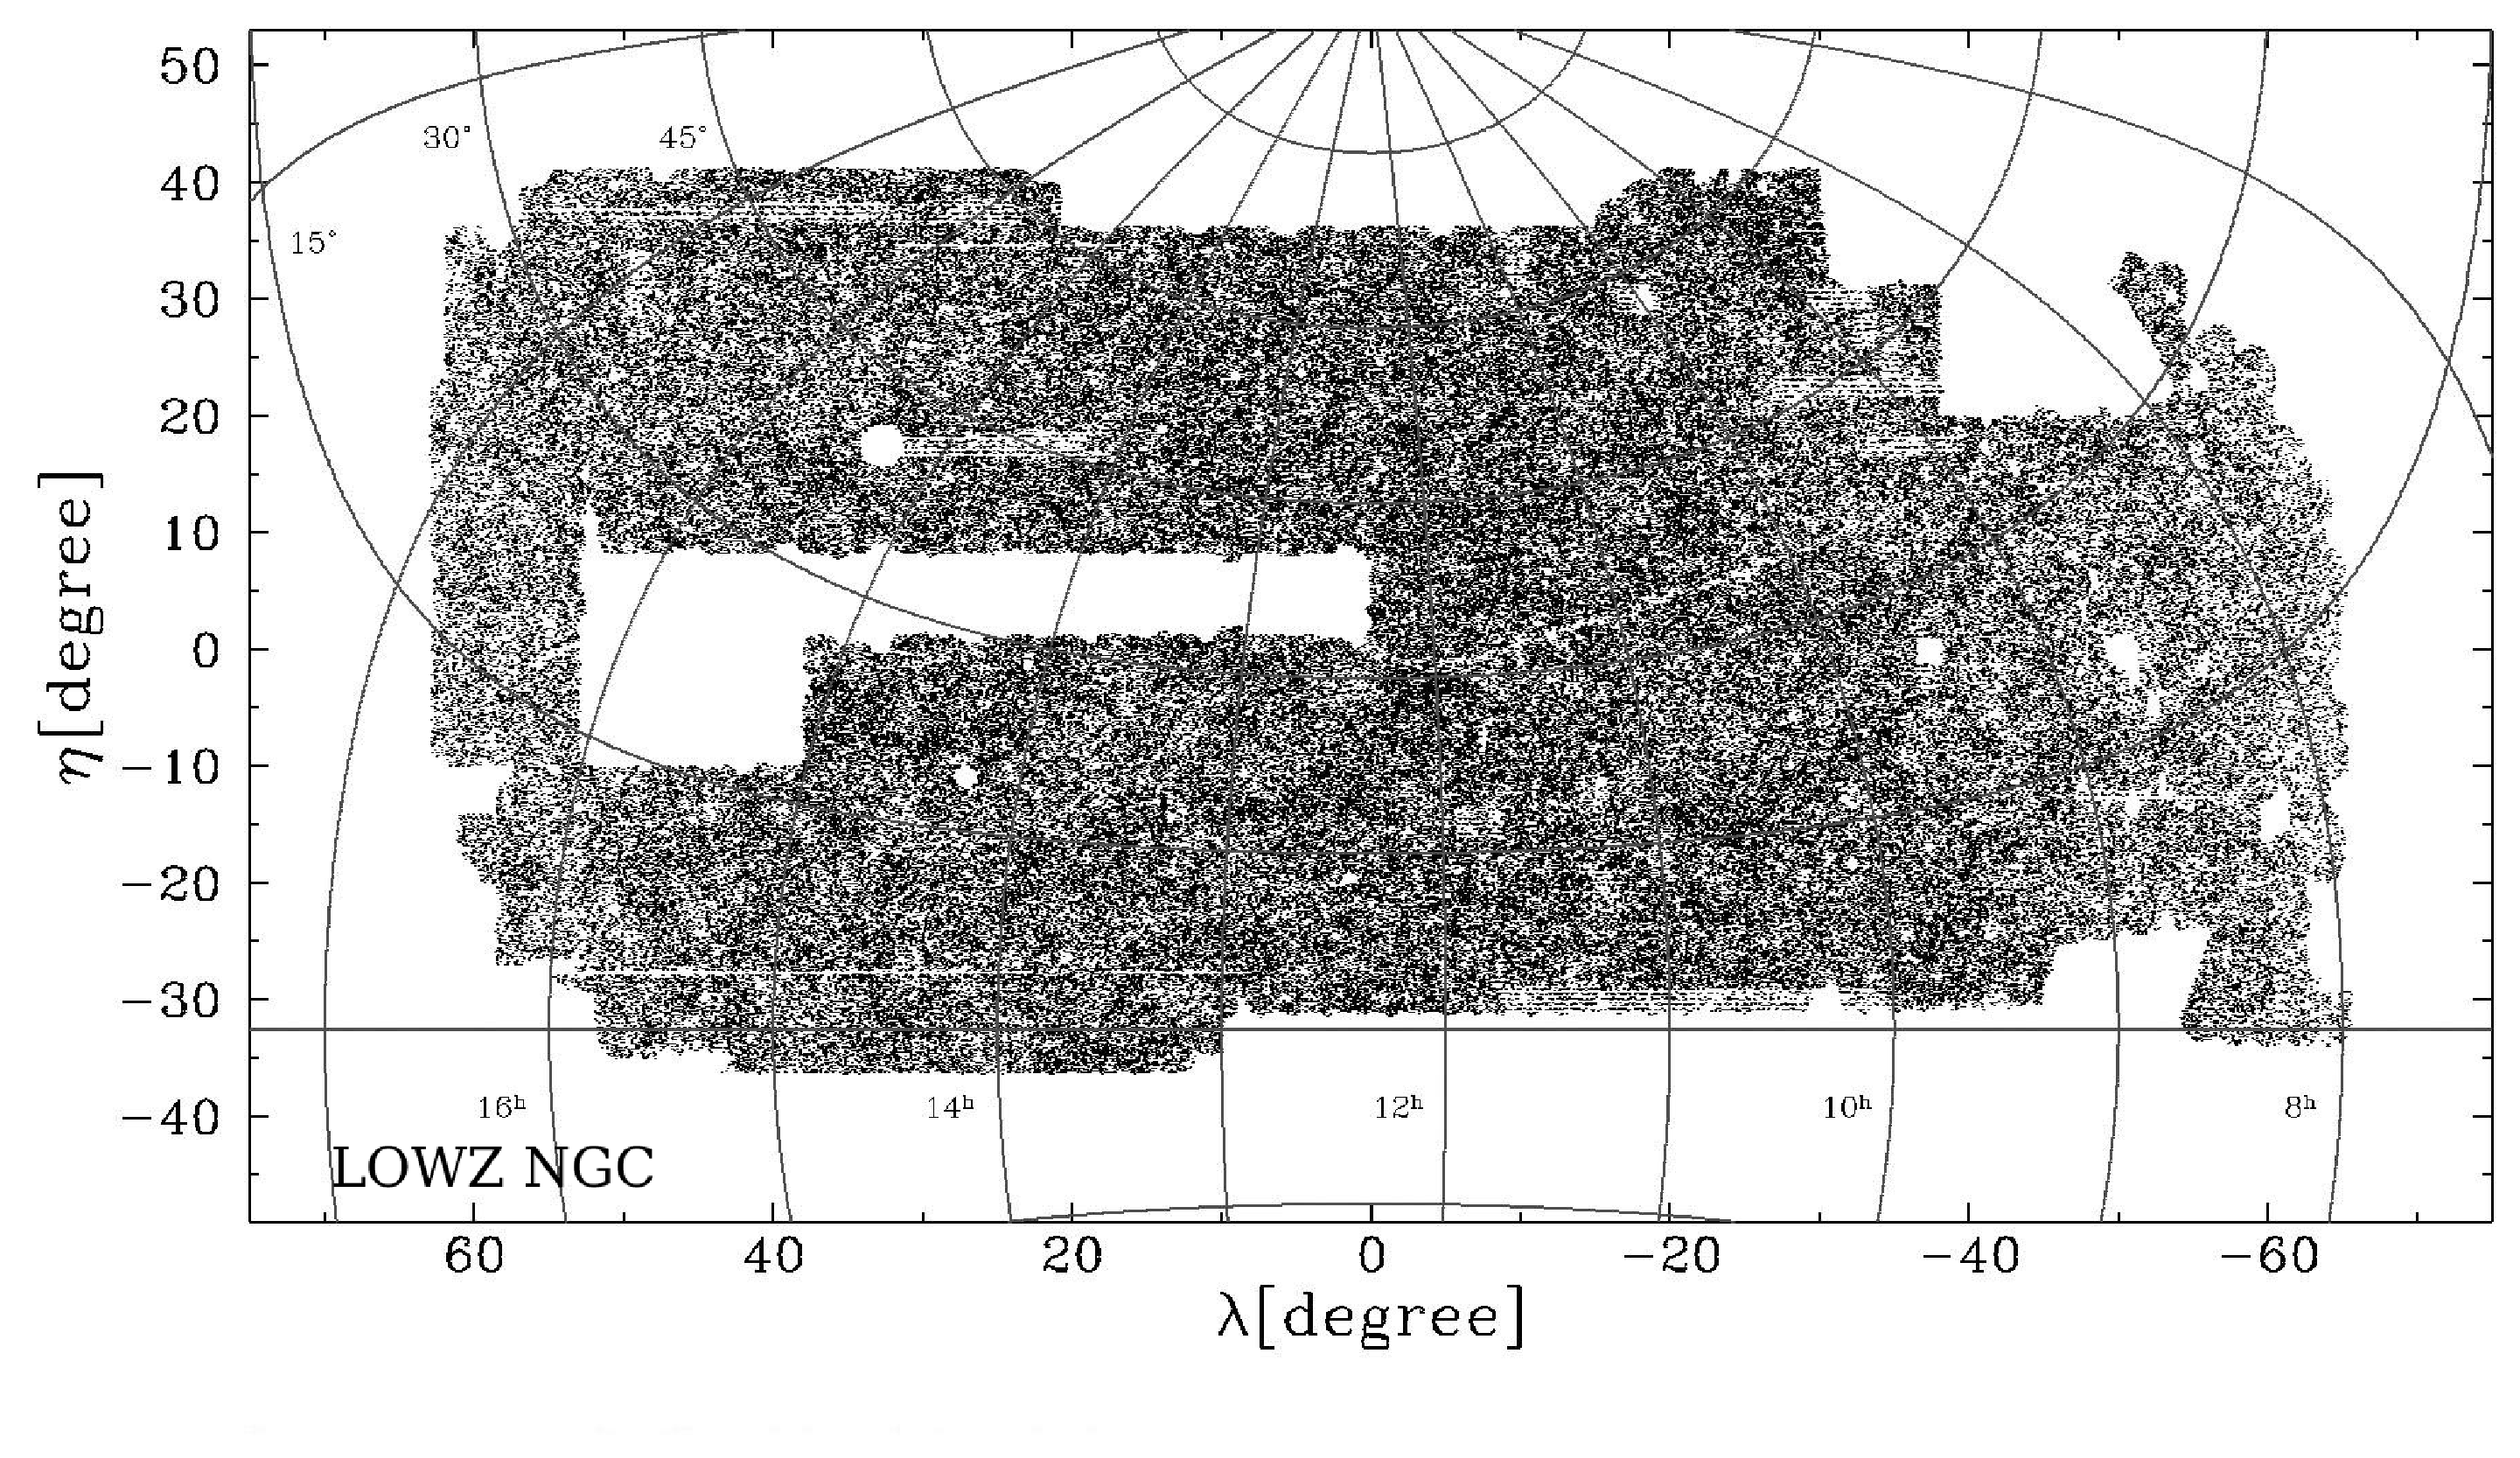
\includegraphics[width=8.5cm]{fig1_0.eps}
   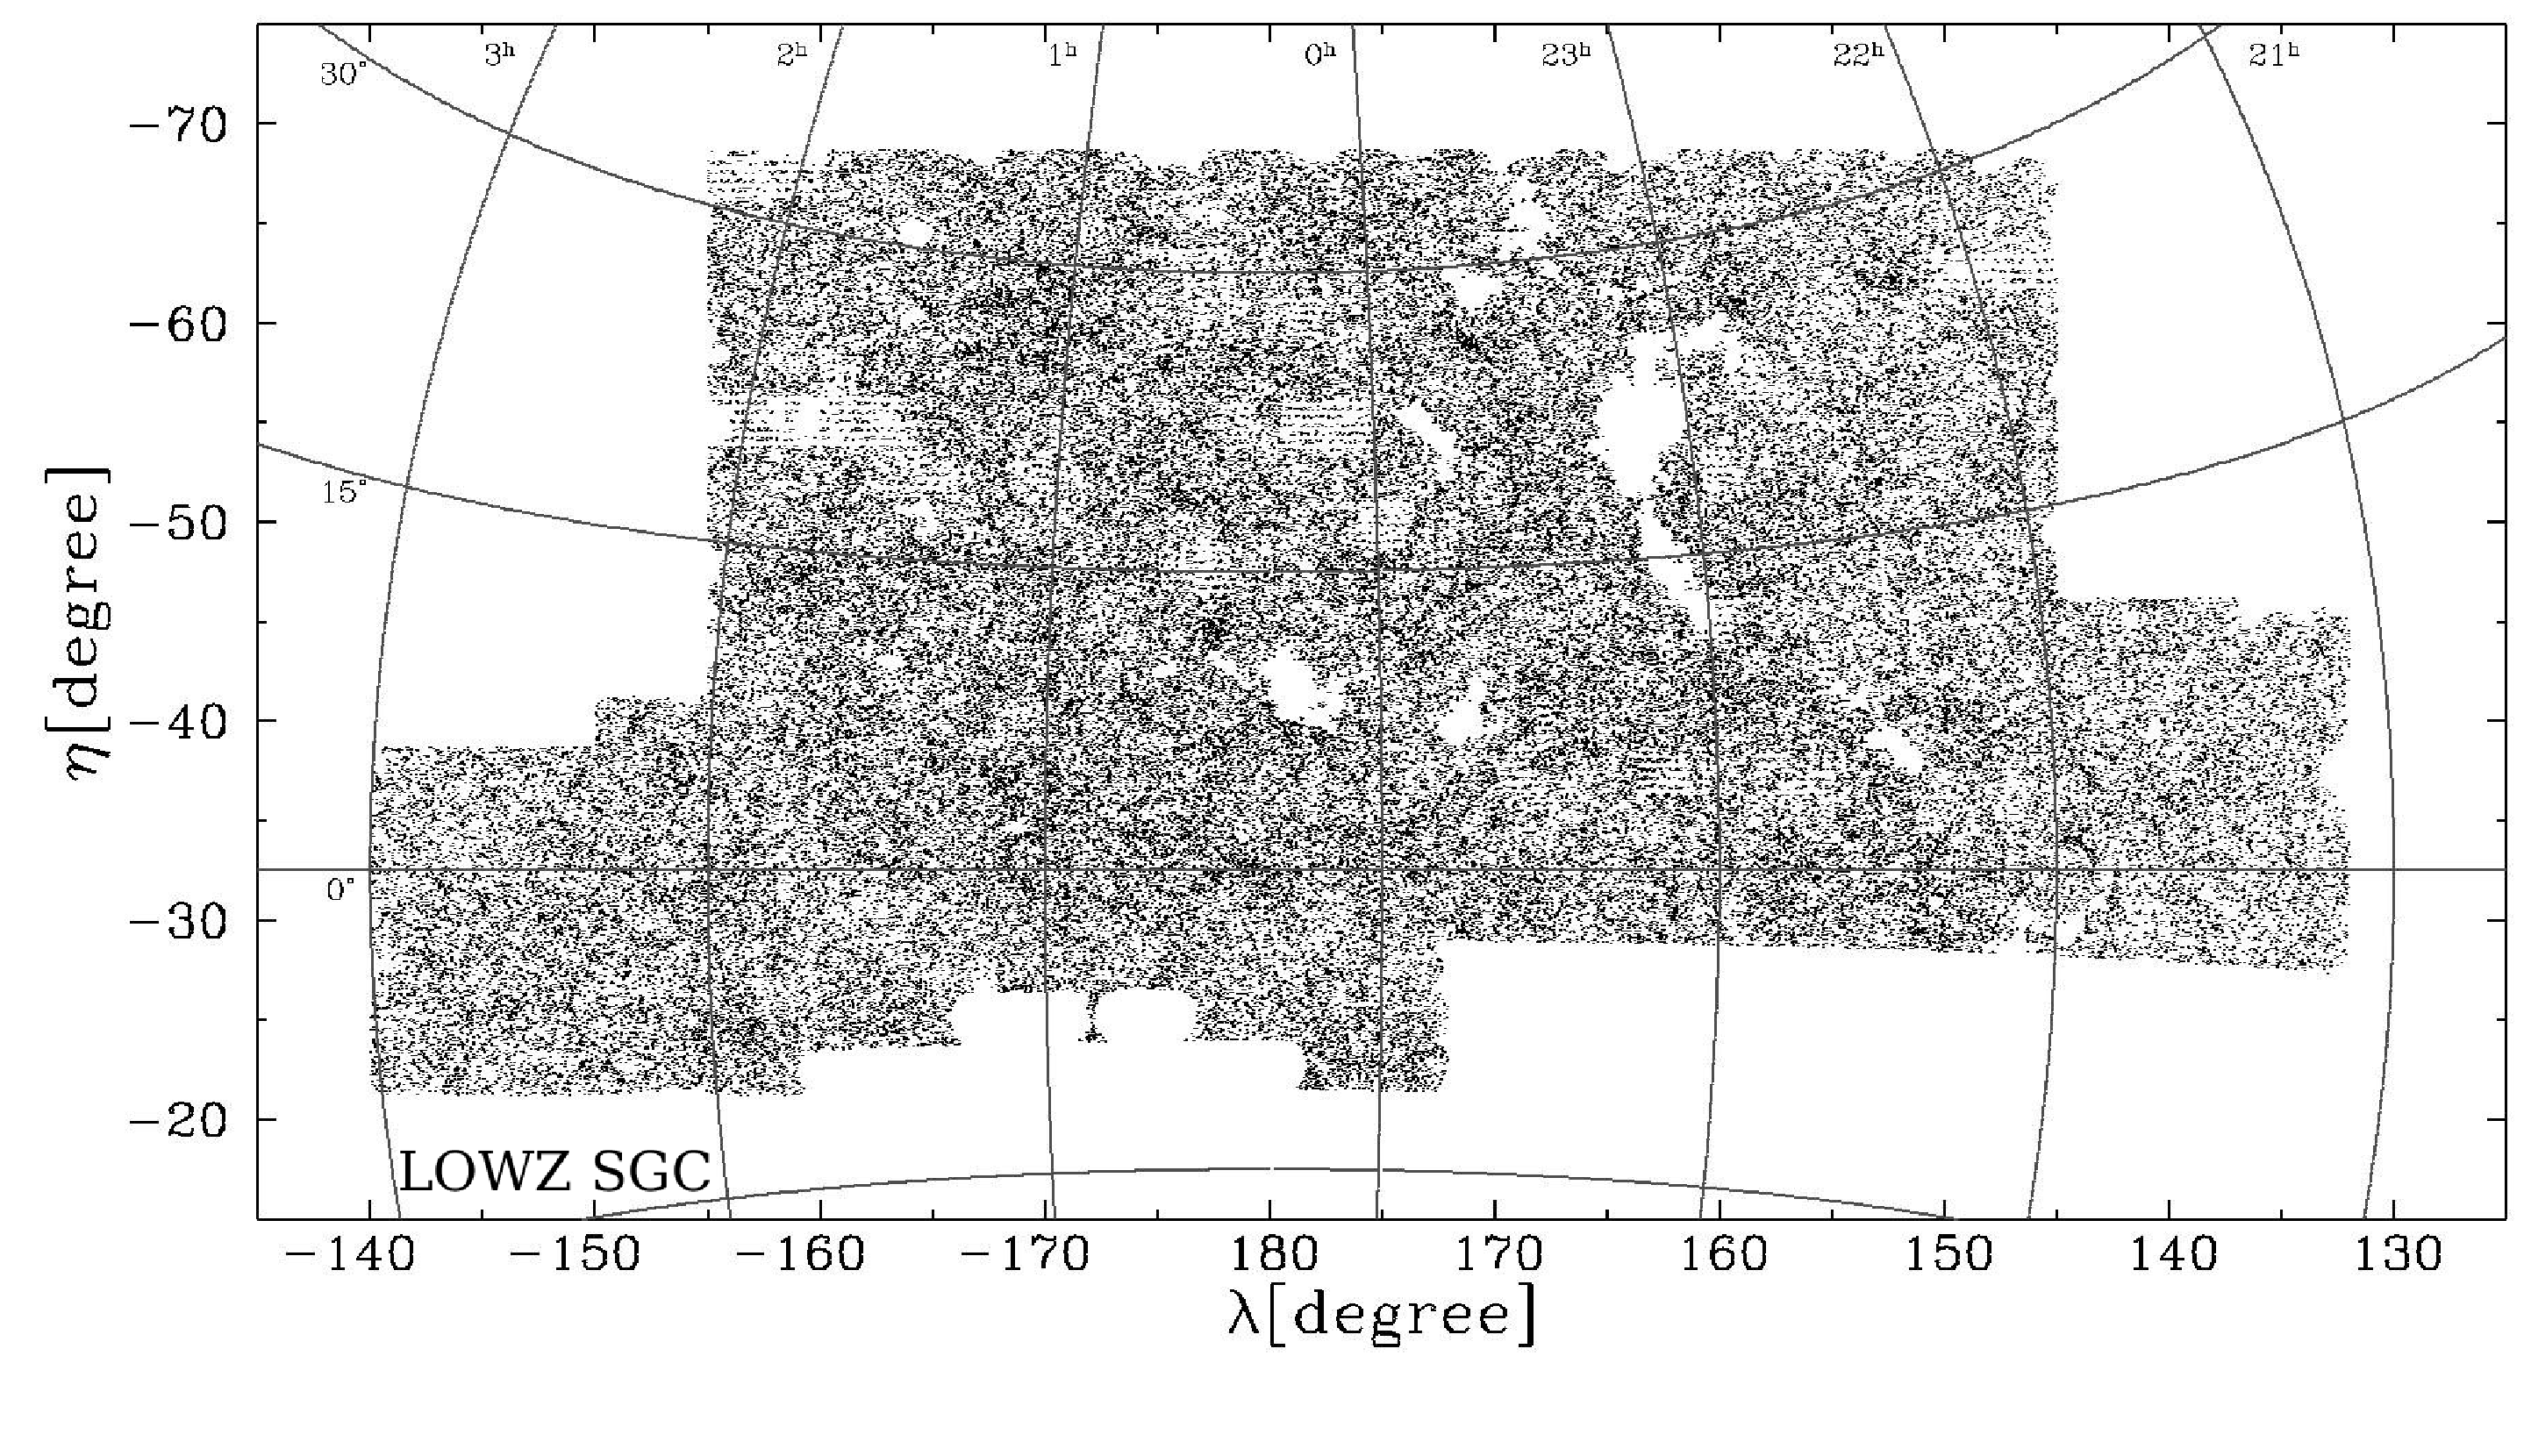
\includegraphics[width=8.5cm]{fig1_1.eps}
   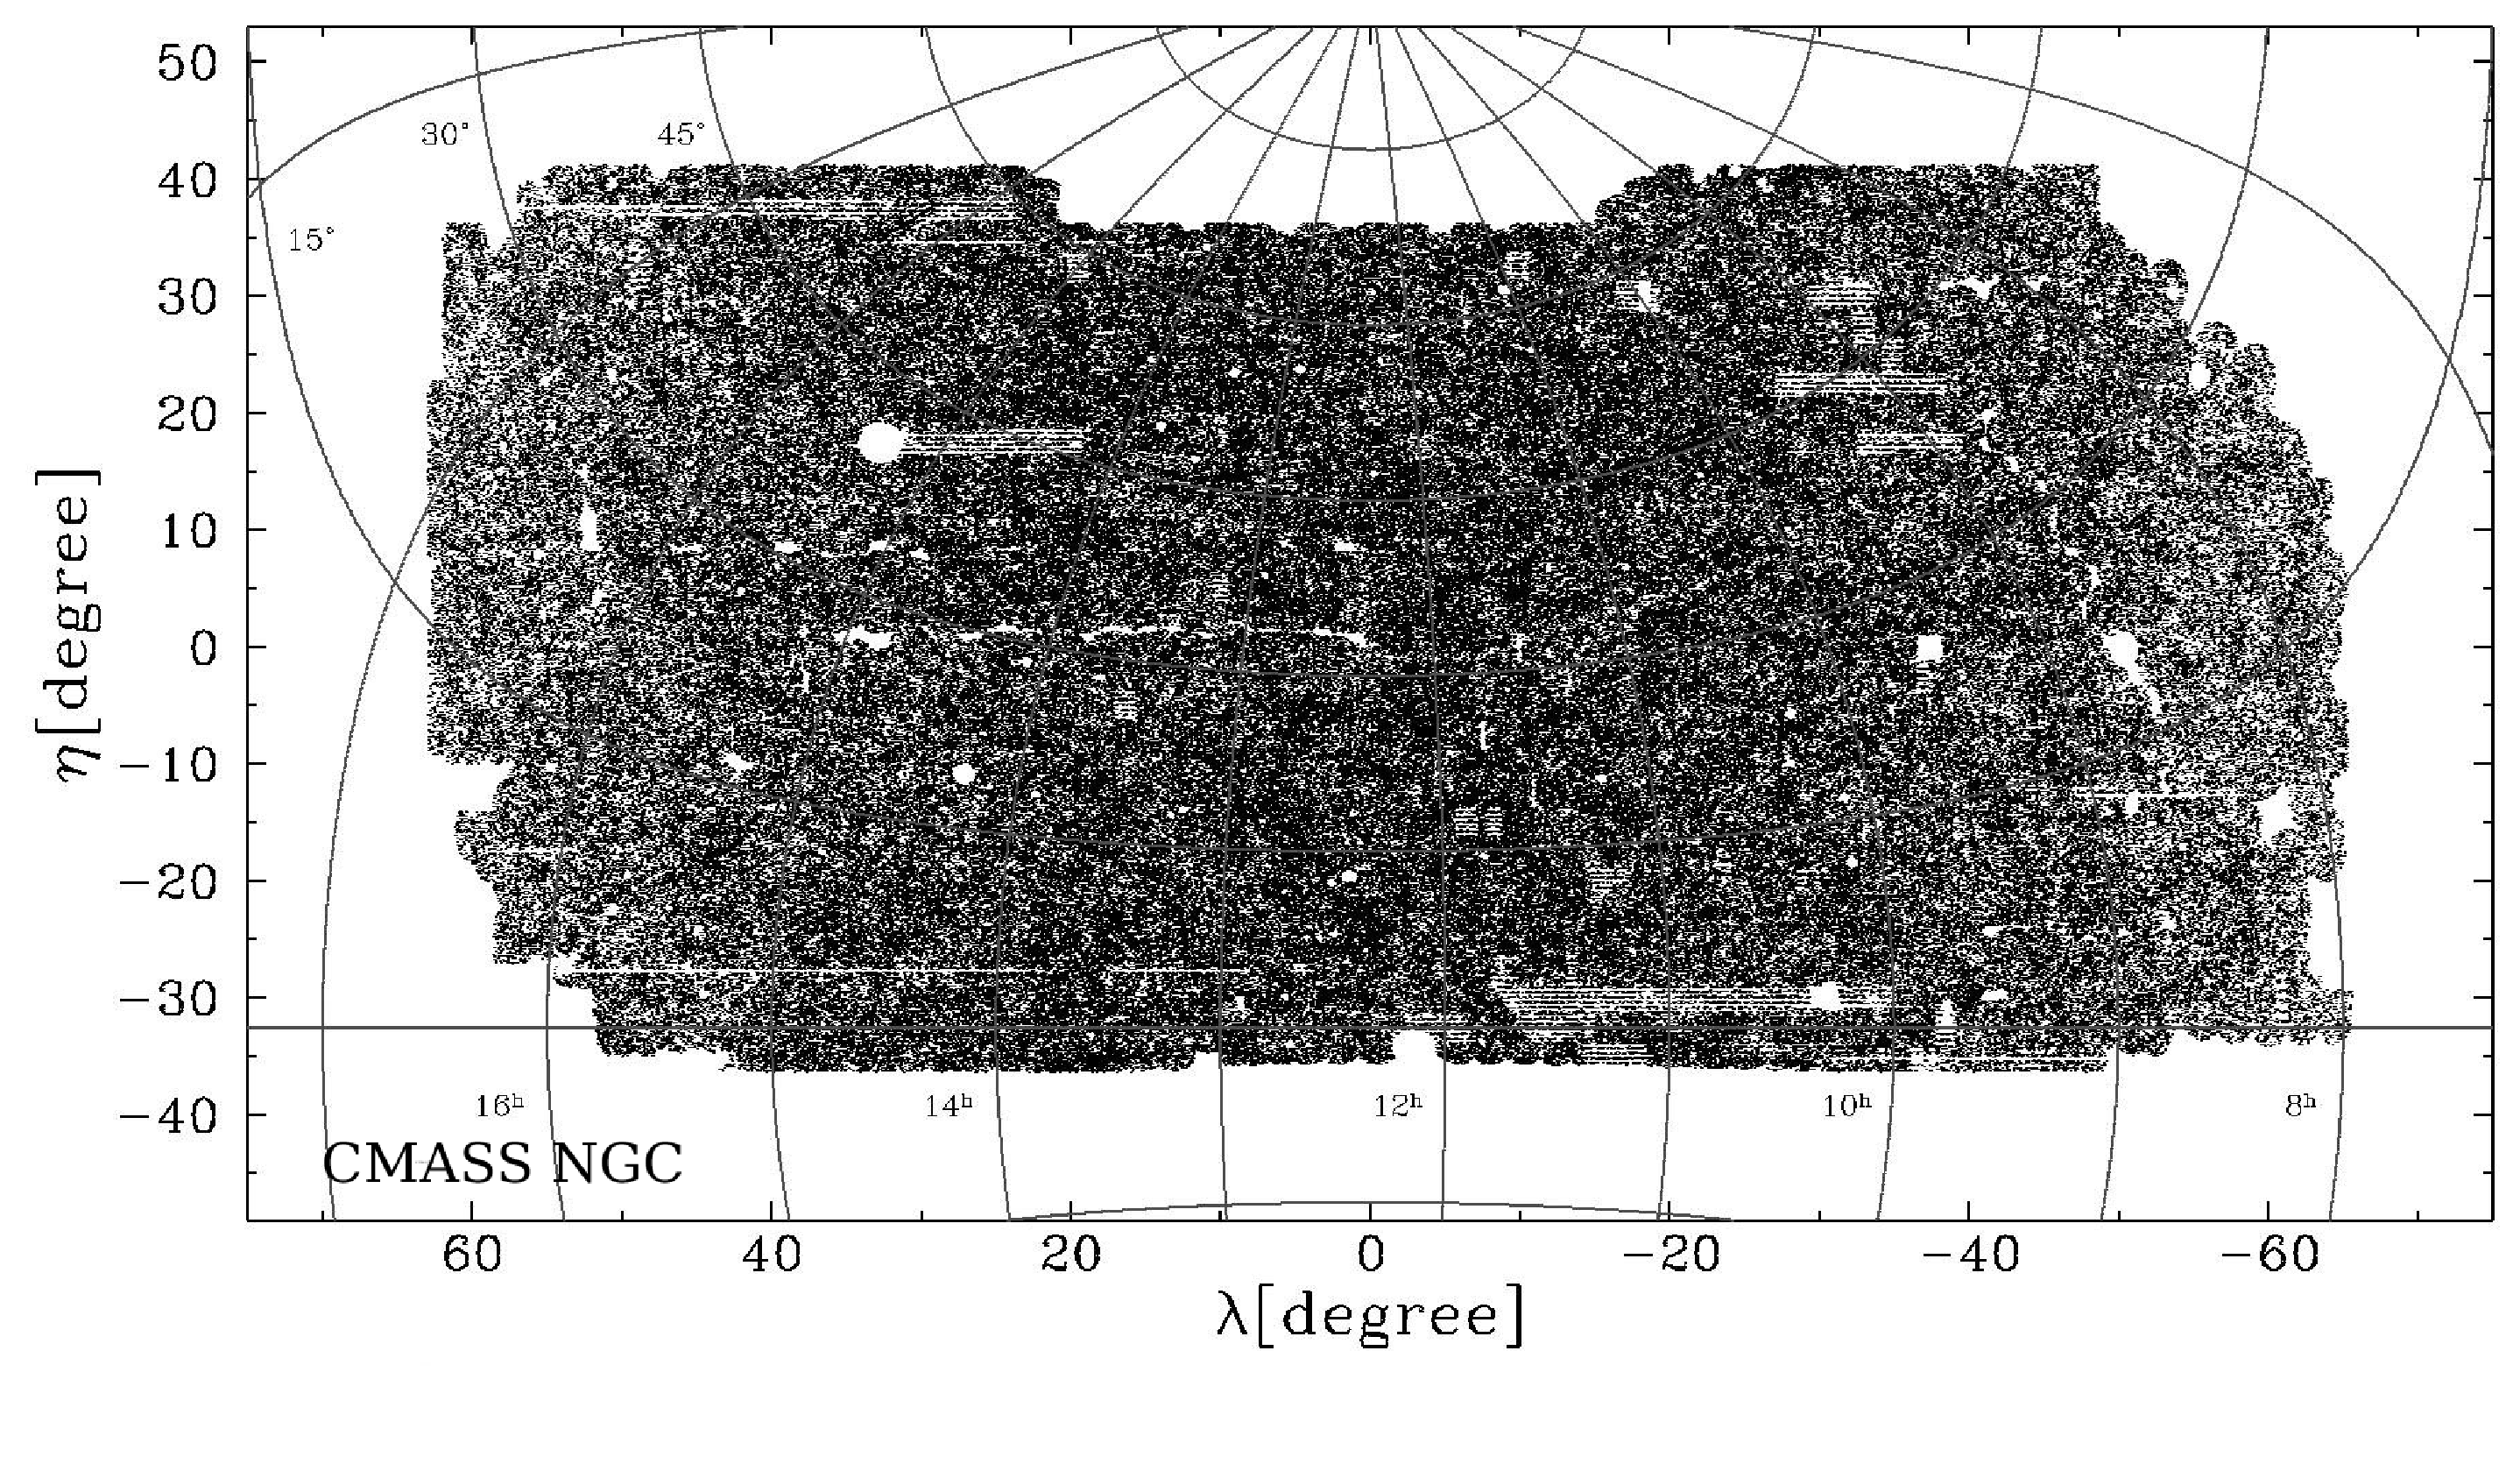
\includegraphics[width=8.5cm]{fig1_2.eps}
   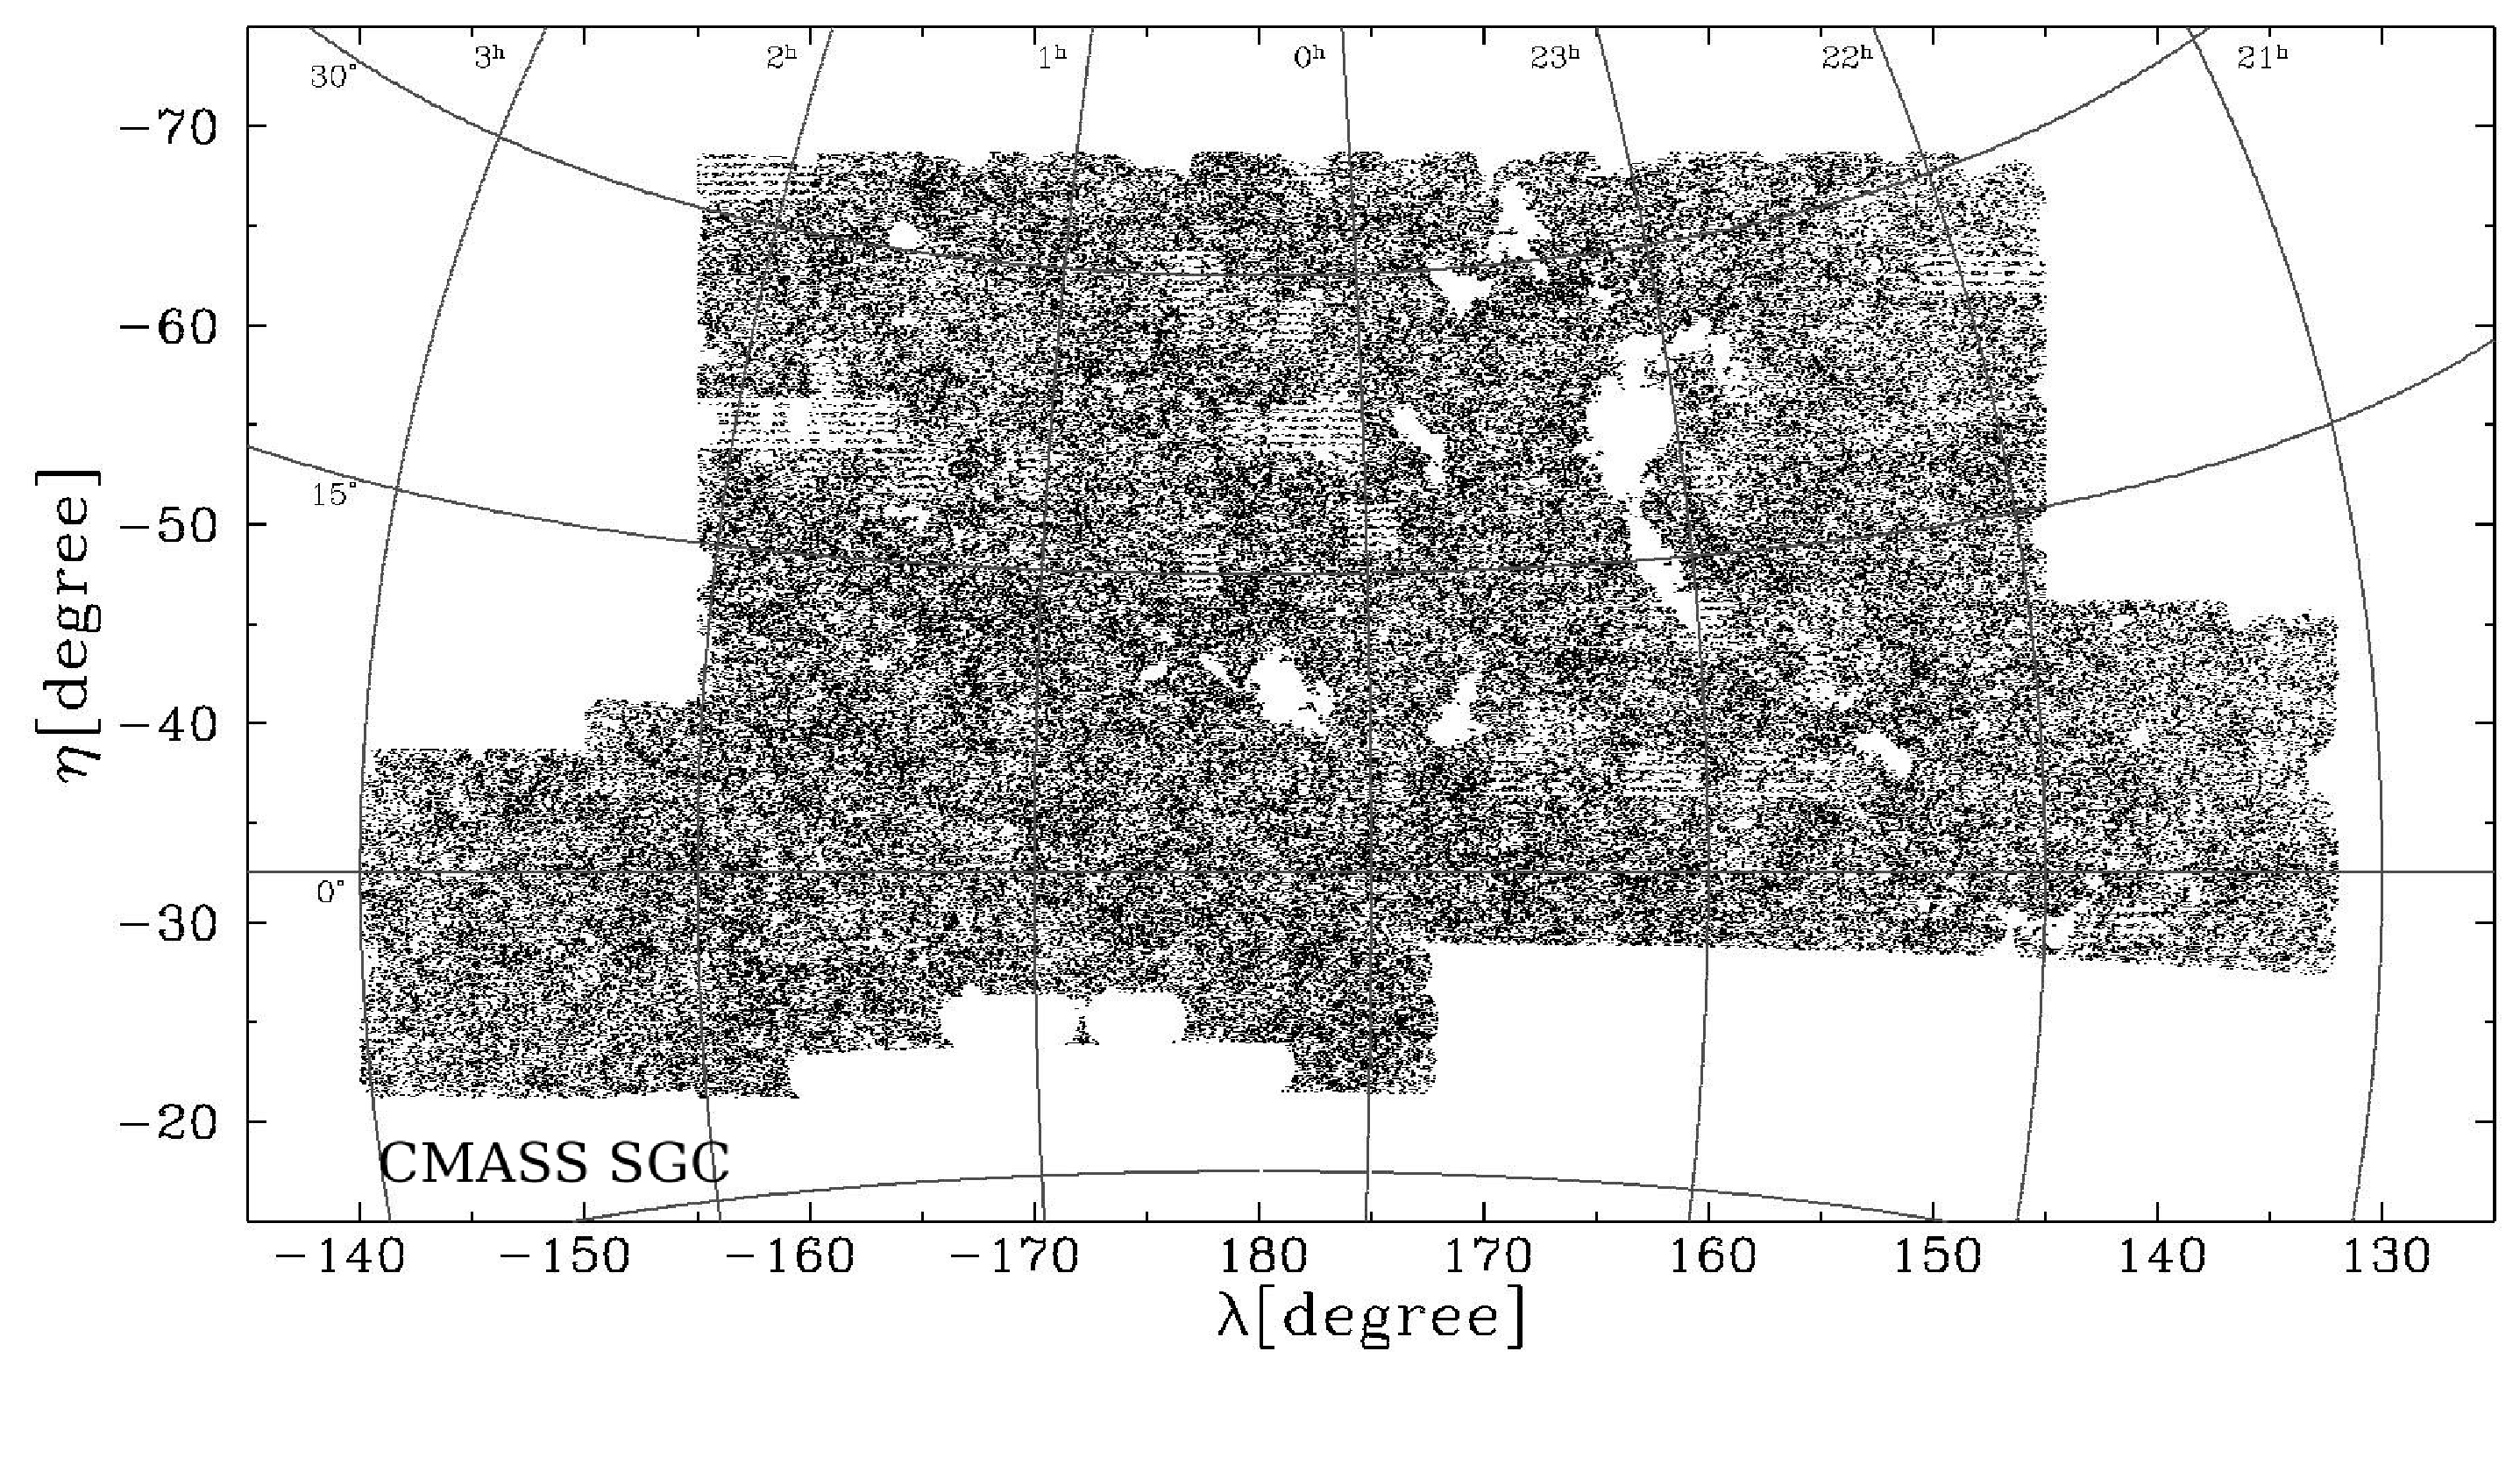
\includegraphics[width=8.5cm]{fig1_3.eps}
   }
   \caption{\label{fig_radec}
   The sky coverage of the LOWZ and CMASS samples in the north and south Galactic caps. 
   The individual points mark position of galaxies in the survey coordinate frame.
   The solid lines mark the right ascension and declination.
   The mean completeness is 97.2\% for the LOWZ sample, shown in the upper panels,
   and 98.8\% for the CMASS sample in the lower panels.
   The effective sky coverage is 8,337 $\rm deg^2$ for LOWZ and 9,376 $\rm deg^2$ for CMASS.
   %Each patch corresponds to a plate,
   %with the color determined by the completeness of that plate.
   See \cite{Reidetal:2016} for more details.
   }
\end{figure*}

The spectroscopic sample of BOSS has two primary catalogues.
%the LOWZ at $z\leq0.4$, and CMASS covering $0.4\leq z \leq 0.7$. %of galaxies.
The LOWZ sample is designed to extend the SDSS-I/II LRG sample to $z\approx 0.4$ and fainter luminosities,
in order to increase the number density of the sample by a factor of 3.
The CMASS sample covers a higher redshift ($0.4\lesssim z \lesssim 0.7$).
It was targeted to be an approximately stellar mass limited sample of massive, luminous galaxies.
The final data release (DR12) samples are described in \cite{Reidetal:2016},
where the details of targeting algorithms and the catalogues are provided.
%The full targeting algorithms used and the method for calculating the galaxy and random catalogues are presented in \citet{Reidetal:2016}, 
%Full details of targeting algorithms and the catalogues are provided in \citep{}, 
%and we do not replicate this here.


%The galaxy survey used two primary target algorithms, 
%selecting samples called LOWZ, with 361\,759 galaxies in the final data release DR12 \citep{dr12} between $0.15<z <0.43$ and CMASS, 
%with 771\,567 galaxies in DR12 between $0.43< z < 0.70$. 
%The full targeting algorithms used and the method for calculating the galaxy and random catalogues are presented in \citet{Reidetal:2016}, 
%which also shows that the samples jointly cover a large cosmic volume $V_{\rm eff}=7.4\,{\rm Gpc}^3$.
%with a number density of galaxies as a function of observed redshift, 
%that ensures that the shot noise does not dominate at BAO (baryon acoustic oscillation) scales. 
%The full targeting algorithms used and the method for calculating the galaxy and random catalogues are presented in \citet{Reidetal:2016}, 
%Full details of the catalogues are provided in \citet{Reidetal:2016}, 
%and we do not replicate this here.

%BOSS is designed to obtain 
%spectra and redshifts of $\sim$1.35 million galaxies 
%(together with 160\,000 quasars and approximately 100\,000 ancillary targets)
%selected from the SDSS imaging.
%The SDSS-I/II data \citep{York et al. 2000} 

%CMASS and LOWZ\,

%We use data from the Sloan Digital Sky Survey \citep[SDSS; ][]{2000AJ....120.1579Y}. 
%SDSS has mapped over one quarter of the sky in five photometric bands down to a limiting magnitude of $r\sim 22.5$. 
%The photometric data is reduced and from it are selected targets for followup spectroscopy. 
%The spectroscopic survey, known as the Baryon Oscillation Spectroscopic Survey (BOSS), 
%is charged with obtaining spectra for 1.35 million galaxies over a 10,000 square degree footprint.



\begin{figure*}
   \centering{
   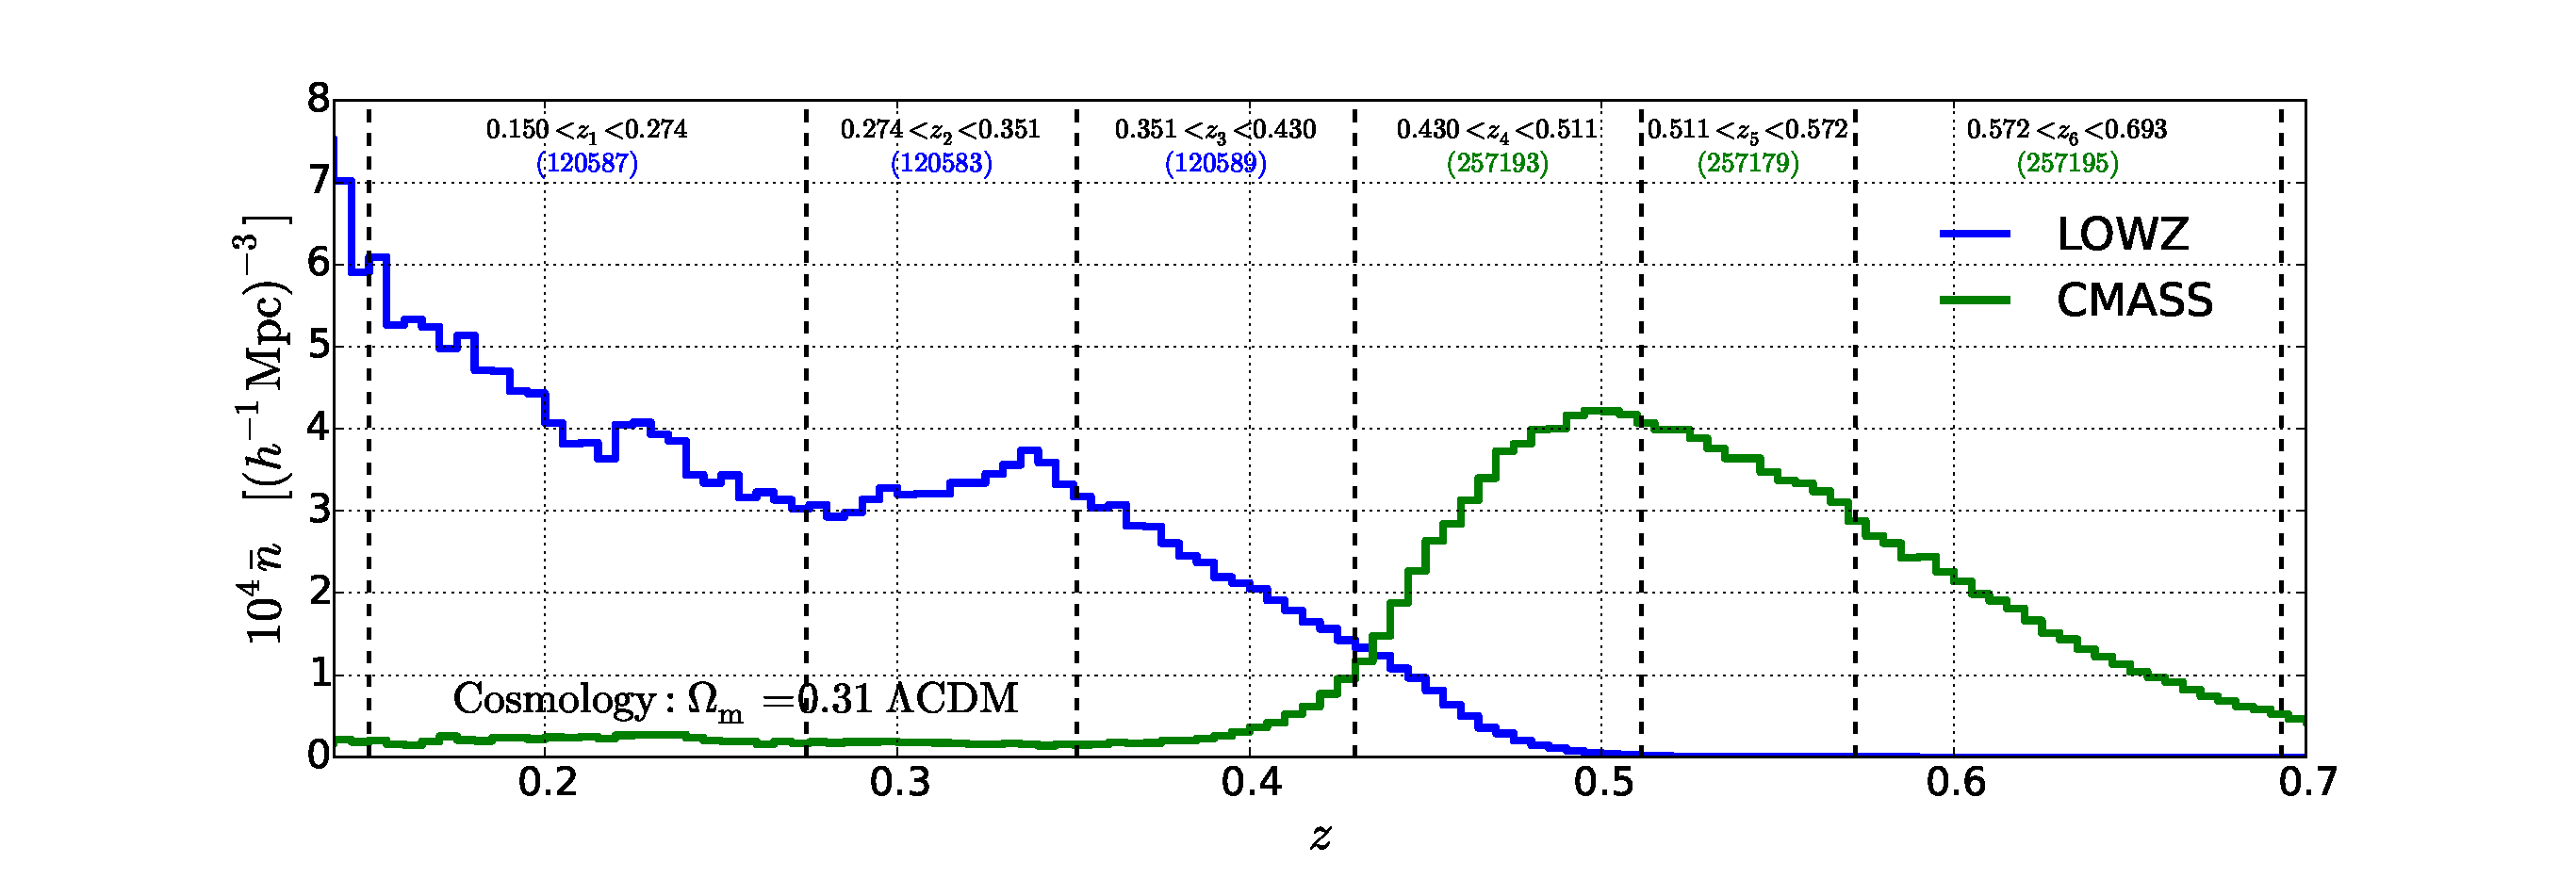
\includegraphics[width=19cm]{fig2.eps}
   }
   \caption{\label{fig_nbar}
      The redshift density distribution of the BOSS DR12 galaxy samples, assuming a $\Lambda$CDM cosmology with $\Omega_m=0.31$.
      The blue and green solid histograms show the distribution of LOWZ and CMASS galaxies respectively. 
      The vertical dashed lines define the six redshift bins that are used to cut the samples.
      Their redshift ranges are listed.
      The number of LOWZ (CMASS) galaxies in the three low (high) redshift bins are presented in the brackets.
      }
\end{figure*}

Figure \ref{fig_radec} presents the sky coverage of the BOSS DR12 samples used in this analysis. 
%The light grey shaded region shows the expected total footprint of the BOSS survey. 
%Colors indicate the spectroscopic completeness.
The mean completeness is 97.2\% for the LOWZ sample, in the upper panels, and 98.8\% for the CMASS sample shown in the lower panels.
   %Each patch of different color corresponds to a plate,
   %with the color determined by the completeness of that plate..
Figure \ref{fig_nbar} shows the galaxy number density of the two samples.
In this analysis we use 361\,759 LOWZ galaxies at $0.15<z <0.43$ and 
771\,567 CMASS galaxies at $0.43< z < 0.693$.
%in total galaxies.
We split the galaxies into six redshift bins: 
three bins in LOWZ ($0.150<z_1<0.274<z_2<0.351<z_3<0.430$), 
and three in CMASS ($0.430<z_4<0.511<z_5<0.572<z_6<0.693$), 
as illustrated in Figure \ref{fig_nbar}.

\begin{figure*}
   \centering{
   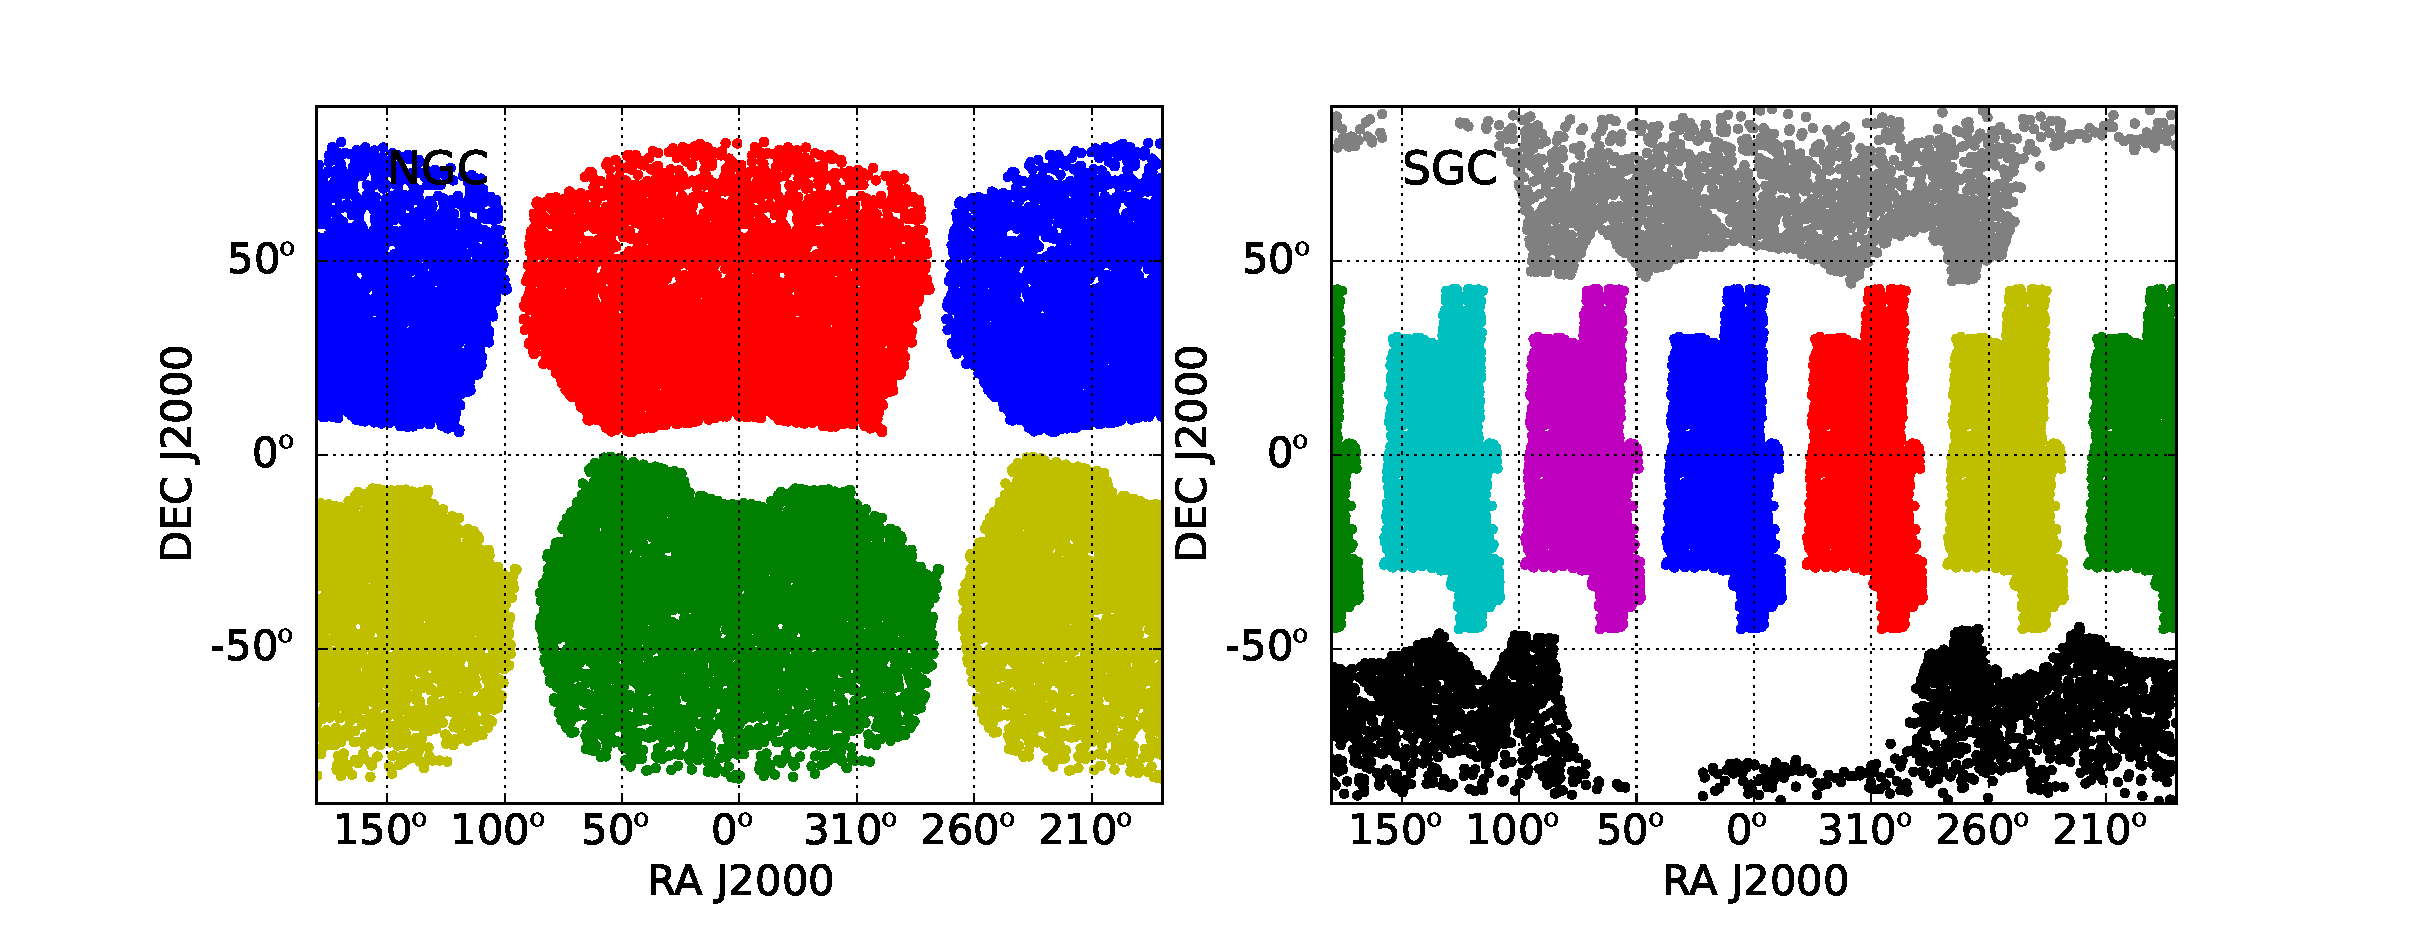
\includegraphics[width=19cm]{fig3.eps}
   }
   \caption{\label{fig_mock}
      Creation of mock galaxy samples for BOSS.
      Using an all-sky mock survey from the HR4 or HR3 simulations,
       we are able to produce four sets of NGC samples or eight sets of SGC samples with non-overlapping sky coverage.
      The individual points are the right ascension and declination of 1\% galaxies drawn from the CMASS samples.
      }
\end{figure*}

Each spectroscopically observed galaxy is assigned several weights to account for observational effects. 
The galaxy weights are constructed from three distinct effects.
%redshift failure, $w_{fail}$, minimum variance, $w_{FKP}$, and angular variation, $w_{sys}$. 
%These weights are described in more detail in \cite{2012MNRAS.427.3435A} and \cite{2012MNRAS.424..564R}. 
Firstly, galaxies lacking a redshift due to fiber collisions 
\footnote{Fiber collisions occur when two objects are close enough together such that two fibers cannot be placed.
In BOSS, the collision radius is 62 $''$.}
or inadequate spectral information are accounted for by reweighting
the nearest galaxy by a weight $w_{\rm fail}=(1+n)$, 
where $n$ is the number of close neighbors without a measured redshift. 
Secondly, all galaxies are assigned `FKP' weights \citep{1994ApJ...426...23F}
%as a function of redshift depending on the number density.
as a function of number density,
to optimize the clustering measurements in the face of shot-noise and cosmic variance.
%according to,
%\begin{equation}
%w^i_{FKP}=\frac{1}{1+n_i(z)P_0},
%\end{equation}
%where $n_i(z)$ is the comoving space density at redshift $z$ and $P_0 \sim P(k=0.1~{\rm $h^{-1}$Mpc}) \sim 2\times 10^{4}h^{-3}{\rm Mpc^3}$, 
%as in \cite{2012MNRAS.427.3435A}. 
The third weight corrects for angular variations of survey completeness and the systematics 
related to the angular variations in stellar density that make detection of
galaxies difficult in over-crowded regions of the sky. %\citep{2012MNRAS.424..564R}. 
The total weight for each galaxy is the product of these three weights, $w_{\rm total}=w_{\rm fail}w_{\rm FKP}w_{\rm sys}$. 

For the statistical analyses, 
random catalogues having the same angular and redshift selection functions as the data 
are provided along with the data \citep{Reidetal:2016}.
%Each random point is assigned with a redshift of measured galaxy randomly drawed from galaxies.
%and a weight given by the $w_{\rm tot}$ of the measured galaxy.
The random points are also weighted but they only include the minimum variance `FKP' weight. 
%50 times as many random points as we have galaxies




\section{The Mock Galaxy Data}
\label{sec:mocks}
%We use HR3 and HR4...
%We use HR4 J08 ...

%Shape of $\\xi$ measured in HR4 very similar to data...
%Shape of 

For LSS studies mock survey samples created from simulations are crucial
for the correction of systematics and covariance estimation.
The Horizon Run simulations are a suite of large volume N-body simulations that 
have resolutions and volumes capable of accurately reproducing the observational statistics of the current major redshift surveys like 
SDSS-III BOSS \citep{park 2005,2009ApJ...701.1547K,horizonrun}.
The HR3 \citep{horizonrun} and HR4 \citep{hr4} simulations are used in our analysis.

From the HR3 and HR4 simulations we have generated all-sky light cone mock galaxy catalogues.
The all-sky spherical mocks are then incorporated with the same fiber collision effect, 
angular masks, and radial selection function with the real observational data,
creating mock surveys of BOSS DR12.

We impose a minimum mass limit varying along with redshift to match the radial density of BOSS samples.
The galaxies of the BOSS DR12 samples do not cleanly distribute above some particular mass boundary;
they always have a fuzzy, blur boundary extending to relatively small values (as an example, see Figure 3 of 
Parihar et al. 2014). %DANGEROUS
%rather than shaprly lying above a certain mass cut, 
Galaxies in the mock samples are systematically more massive than those from observations;
We will discuss the effect of this discrepancy in Sec. \ref{sec:caveats}.


\subsection{Horizon Run 4}

The HR4 simulation  \citep{hr4} used a box size $L={3150}$ $h^{-1}$Mpc, 
and $N=6300^3$ particles.  
The simulation used the second order Lagrangian perturbation theory (2LPT) initial conditions at $z_{i}=100$ and a WMAP5 cosmology
$(\Omega_{b},\Omega_{m},\Omega_\Lambda,h,\sigma_8,n_s)$  = (0.044, 0.26, 0.74, 0.72, 0.79, 0.96) \citep[]{komatsu 2011}, 
yielding a particle mass of $m_{p} \simeq 9.02 \times 10^9 \hMsun$.
This starting redshift, combined  with 2LPT initial conditions, ensures an accurate mass function and power spectrum \citep{2014NewA...30...79L}. 

Mock galaxy samples are produced from the HR4 simulation by using a modified version of the one-to-one correspondence scheme \citep{hong2016}. 
The most bound member particles (MBPs) of simulated halos are adopted as the tracer of galaxies rather than the subhalos,
and the merger timescale is taken into account in the lifetime of merged halos.
We built the merger trees of simulated halos by tracking their MBPs from $z = 12$ to 0.
When a merger event occurs, we calculate the merger timescale described in \cite{jiang2008} (hereafter J08)
to determine when a satellite galaxy is completely disrupted.
%We modeled the position and the velocity of a galaxy from the position and velocity of its corresponding MBP.
By using the abundance matching, 
we modeled the luminosity of a central/isolated galaxies from their current mass
and of satellite galaxies 
from their mass at the time of infall.

\cite{hong2016} compared the 2pCF of our mock galaxy sample at $z = 0$ to the SDSS DR7 volume-limited galaxy sample \citep{zehavi2011}.
%When a typical subhalo-galaxy correspondence scheme is applied, 
%the 2pCF from our simulation is smaller than the observation and does not show a proper Finger-of-God (FOG) feature in our simulation resolution. 
%We found that %the %2pCF of our galaxy sample agrees well with the observation.
The simulated 2pCF shows a similar finger of god (FOG) feature \citep{FOG} as the observation in the contour map, 
and the projected 2pCF agrees with the observation within 1$\sigma$ deviation on scales greater than 1 ${h^{-1}}$Mpc.


%As will be introduced in the next section, 
The HR4 simulation yield one all-sky light cone mock galaxy catalogue reaching $r=3\,150$ ${h^{-1}}$Mpc.
As shown in Figure \ref{fig_mock},
from one all-sky survey, 
we are able to create four sets of non-overlapping north Galactic cap (NGC) samples for CMASS and LOWZ, 
or eight sets of non-overlapping south Galactic cap (SGC) samples.
In this paper we use these simulated galaxies for the estimation of the systematics in the 2pCF of the observed galaxies.
%We create four north 

\begin{figure*}
   \centering{
   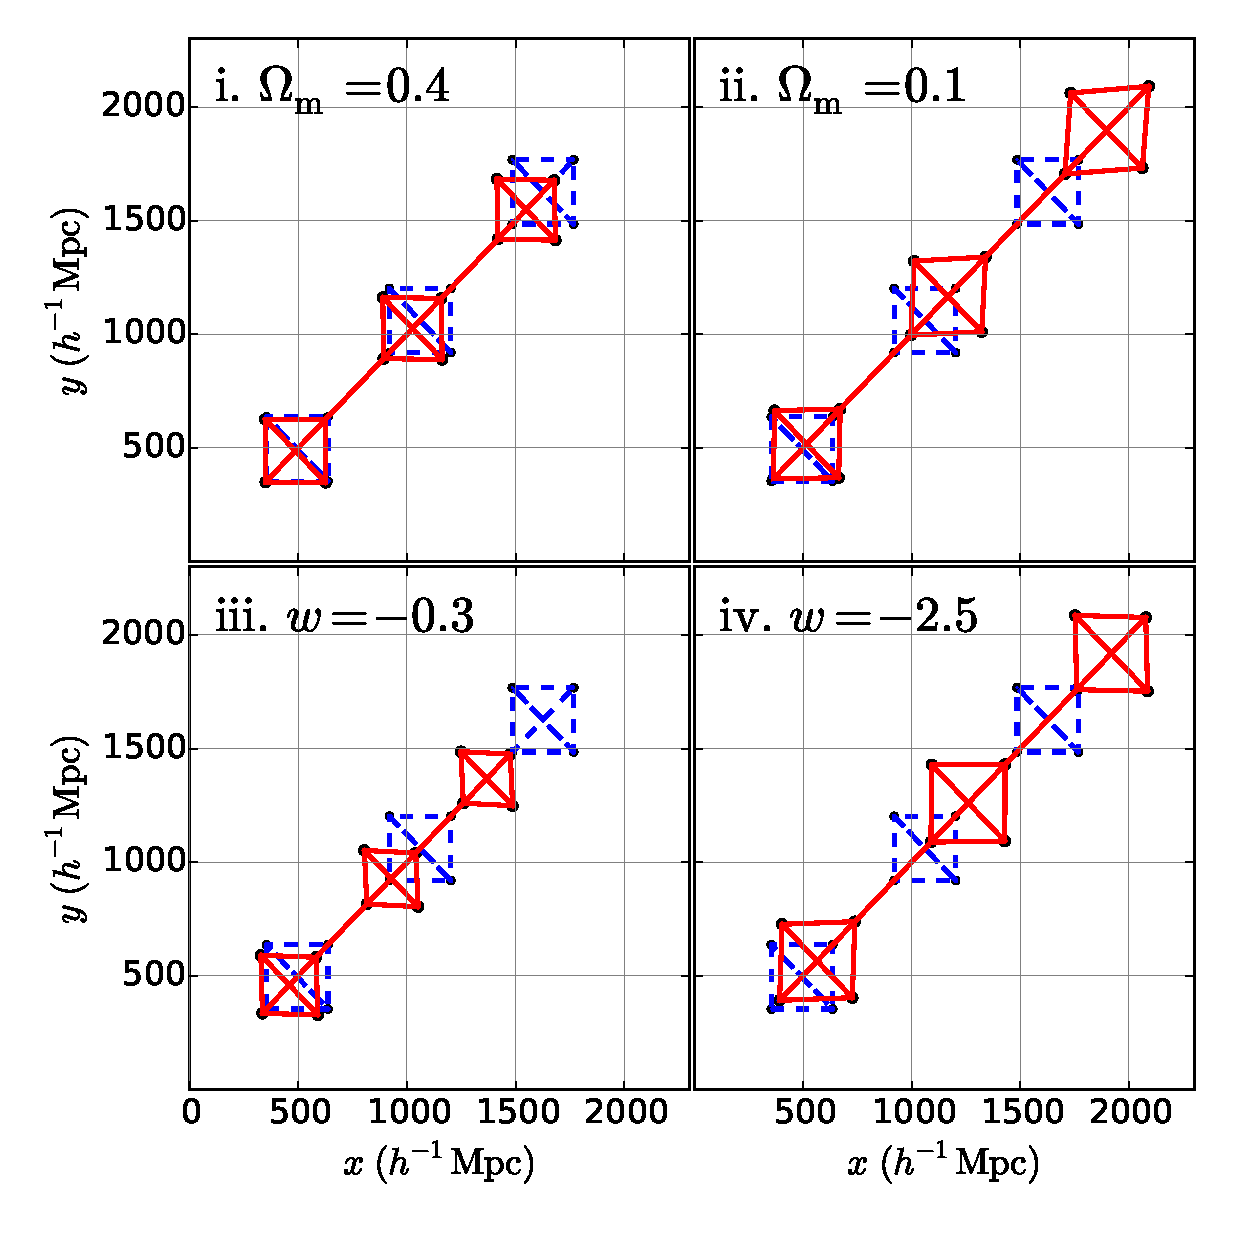
\includegraphics[height=8cm]{fig4_0.eps}
   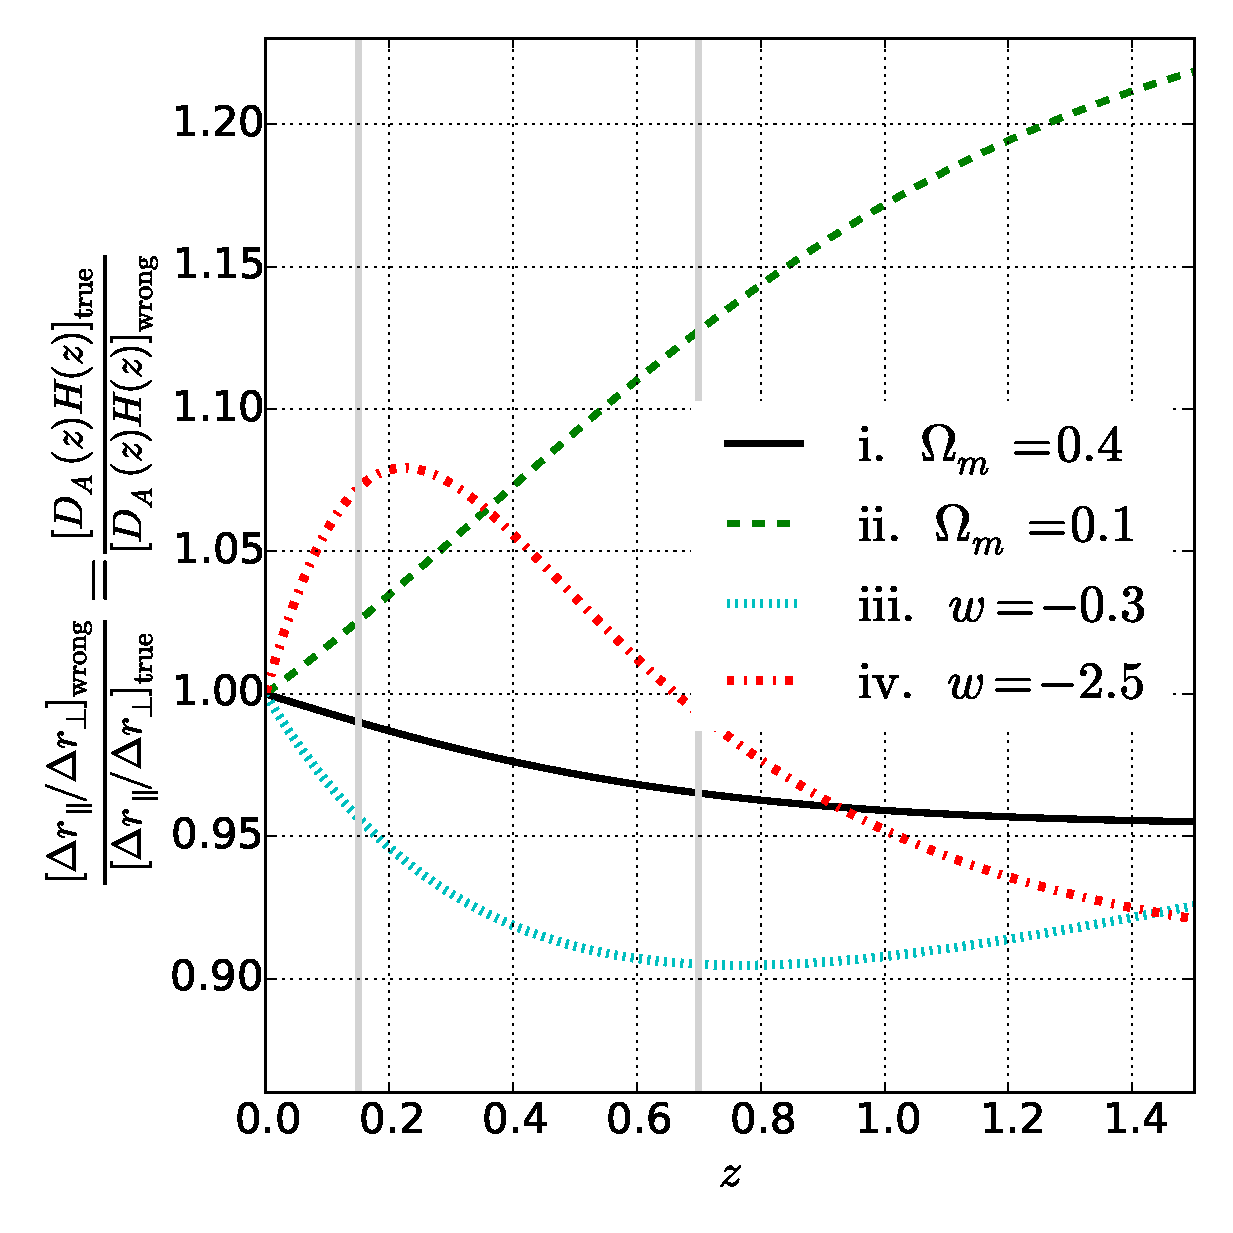
\includegraphics[height=8cm]{fig4_1.eps}
   %\includegraphics[height=7cm]{FVol.eps}
   %\includegraphics[height=8cm]{xy.eps}
   %\includegraphics[height=8cm]{smu.eps}
   }
   \caption{\label{fig_xy}
   %Apparent distortion of objects in four wrongly assumed cosmologies, assuming a true cosmology of .
   The redshift dependence of the AP effect in four incorrect cosmologies,
   assuming that the true cosmology is $\Omega_m=0.31$, $w=-1$.
   The left panel shows the apparent distortion of four perfect squares,
   measured by an observer located at the origin.
   The apparently distorted shapes are plotted in red solid lines.
   The underlying true shapes are indicated in blue dashed lines.
   The right panel displays the degree of the shape distortion, as described by Equations (\ref{eq:stretch}).
   The BOSS DR12 galaxies used in our analysis have a redshift coverage of $0.15 < z < 0.693$ (marked 
   by the gray vertical lines). Clearly, the magnitude of the shape distortion due to AP changes with redshift.
   %measured by an observer located at the origin.
   %For reference, blue dashed squares show their shapes and positions in the true cosmology.
   }
\end{figure*}



\subsection{Horizon Run 3}
%In our analysis we also mock surveys constructed from one of the Horizon Run simulations, HR3.

As in HR4, HR3 also adopts a flat-space $\Lambda$CDM cosmology with the WMAP 5 year parameters.
The simulation was made in a cube of volume $(10.815\  h^{-1}{\rm{Gpc}})^3$
using $7120^3$ particles with particle mass of $1.25\times 10^{11}$\hMsun.
The simulations were integrated from $z=27$ and reached $z=0$ after making $N_{\rm step}=600$ global timesteps.
The collapsed high-density regions were identified using the Friend-of-Friend algorithm with the linking length of 0.2 times the mean particle separation.
The physically self-bound (PSB) subhalos that are gravitationally self-bound and tidally stable \citep{kim and park 2006} 
are identified and used as galaxy proxies.
The PSB halo finder is a group-finding algorithm which can efficiently identify halos located even in crowded regions. 
This method combines two physical criteria such as the tidal radius of a halo and the total energy of each particle to find member particles.
The group velocity of member particles is adopted as the peculiar velocity of each PSB subhalo.

%This provides a substantial increase in the similarity between simulation and observational data,
%as these dark matter subhalos are sites for galaxy formation.
%LRG (Xiao: is it OK to change all the ``LRG'' to ``galaxy''?) formation.

To simulate the SDSS survey,
HR3 places 27 observers evenly within its cubical volume and allows
each observer to survey out to a redshift of 0.7
\footnote{In the analysis we choose the maximal redshift as 0.693 rather than 0.7. 
%The lightcone data created from HR3 simulations have cosmological redshift limit of $z<0.7$. 
The outer boundary of the mock survey becomes fuzzy due to the peculiar velocity effect 
on the galaxy redshifts (Eq. (\ref{eq:zvpeu})).
A population of galaxies, that are expected to enter the $z<0.7$ region from the outside, is missing.
%(these $z>0.7$ galaxies have a peculiar velocity toward us and 
%their observed redshfits become lower than 0.7).
To avoid this problem we set the maximal redshift at 0.693, 
23.3 $h^{-1}{\rm Mpc}$ away from $z=0.7$.}, 
creating 27 samples of independent, non-overlapping spherical regions.
From the 27 spherical light cone `galaxy' catalogues, 
we created 72 non-overlapping survey samples 
\footnote{Using the 27 spherical light cones, we create 72 sets of NGC samples from 18 light cones, 
and 72 sets of SGC samples from the other 9 light cones.}
simulating BOSS DR12 within the redshift range of $0.15< z< 0.693$.
%As will be described in the next section, 
These mock surveys are used to estimate the covariance of the 2pCF in our analysis.



\section{AP Effect in Incorrect Cosmologies}
\label{sec:APeffect}

%Considering we are Let us consider an object in the Universe with certain size and shape.
%Its observed redshift span $\Delta z$ and angular size $\Delta \theta$ are related with the comoving sizes by
This section illustrates the AP effect when an incorrect cosmological model is used to calculate the distances of galaxies. Similar illustrations have been provided in \cite{Li2014,Li2015}.

Suppose that we probe the shape and volume of an object in the Universe,
which spans $\Delta z$ in redshift and $\Delta \theta$ in angle.
Its comoving sizes in the radial and transverse directions are given by
\begin{eqnarray}\label{eq:distance}
& &\Delta r_{\parallel} = \frac{c}{H(z)}\Delta z,\nonumber\\
& &\Delta r_{\bot}=(1+z)D_A(z)\Delta \theta,
\end{eqnarray}
where $H$ is the Hubble parameter and $D_A$ the proper angular diameter distance.
In the particular case of a flat Universe with constant dark energy EoS, they take the forms of
\begin{eqnarray}\label{eq:HDA}
& &H(z) = H_0\sqrt{\Omega_ma^{-3}+(1-\Omega_m)a^{-3(1+w)}},\nonumber\\
& &D_A(z) = \frac{c}{1+z}r(z)=\frac{c}{1+z}\int_0^z \frac{dz^\prime}{H(z^\prime)},
\end{eqnarray}
where $a=1/(1+z)$ is the cosmic scale factor,
$H_0$ is the present value of Hubble parameter and $r(z)$ is the comoving distance.

In case we adopted an incorrect set of cosmological parameters in Equation (\ref{eq:HDA}),
the inferred $\Delta r_{\parallel}$ and $\Delta r_{\bot}$ are also incorrect,
resulting in distorted shape (AP effect) and wrongly estimated volume (volume effect).
The degree of variations in shape and volume are
\begin{equation}\label{eq:stretch}
 %{\rm Degree\ of\ LOS\ stretch\equiv}
 %{\rm rat}_{\rm LOS\ stretch}\equiv
 \frac{[\Delta r_{\parallel}/\Delta r_{\perp}]_{\rm wrong}}{[\Delta r_{\parallel}/\Delta r_{\perp}]_{\rm true}} =
  \frac{[D_A(z)H(z)]_{\rm true}}{[D_A(z)H(z)]_{\rm wrong}} 
\end{equation}
\begin{equation}\label{eq:volume}
 %{\rm Degree\ of\ volume\ magnification \equiv}
 %{\rm rat}_{\rm volume\ mag}\equiv
 \frac{{\rm Volume}_{\rm wrong}}{{\rm Volume}_{\rm true}}
 = \frac{[\Delta r_{\parallel}(\Delta r_{\perp})^{2}]_{\rm wrong}}{[\Delta r_{\parallel}(\Delta r_{\perp})^{2}]_{\rm true}}
 = \frac{[D_A(z)^2/H(z)]_{\rm wrong}}{[D_A(z)^2 / H(z)]_{\rm true}},
\end{equation}
where ``true'' and ``wrong'' denote the values of quantities in the true cosmology and incorrectly assumed cosmology.
From the AP and volume effects, we can constrain  $D_A(z)H(z)$ and $D_A(z)^2 / H(z)$, respectively.


The apparent distortion of objects due to incorrect cosmological parameters is illustrated in the left panel of Figure \ref{fig_xy}.
Suppose that the true cosmology is a flat $\Lambda$CDM model with the present density parameter $\Omega_m=0.31$
and standard dark energy EoS $w=-1$ \citep[the best $\Lambda$CDM model determined by Planck 2015 results][]{Planck2015}.
%(the best $\Lambda$CDM model determined by Planck 2015 results \citep{Planck2015}).
If we distributed three square objects at various distances from 500 to 2,000 $h^{-1}$Mpc,
and had an observer located at the origin measure their redshifts and compute their positions and shapes 
using redshift-distance relations of four incorrect cosmologies:
\begin{enumerate}[label=(\roman*)]
\item $\Omega_m=0.4$, $w=-1$,
\item $\Omega_m=0.1$, $w=-1$,
\item $\Omega_m=0.31$, $w=-0.3$,
\item $\Omega_m=0.31$, $w=-2.5$,
\end{enumerate}
the mismatch between the true and assumed cosmology will cause the shapes of the squares appear distorted.
In the cosmological models (ii) and (iv) the squares are stretched in the line of sight (LOS) direction (hereafter ``LOS shape stretch''),
%and magnification of the volume (hereafter ``volume magnification''), 
while in the models (i) and (iii) we see opposite effects of LOS shape compression.


The right panel of Figure \ref{fig_xy} presents the degree of shape distortion as a function of redshift. 
In cosmology (i) and (iii), $\frac{[D_A(z)H(z)]_{\rm true}}{[D_A(z)H(z)]_{\rm wrong}}$ have values less than 1, 
indicating LOS shape compression,
while in cosmology (ii) the curve lies above 1, 
corresponding to an LOS shape stretch.
The effect in cosmology (iv) is more subtle. 
There is a transition from LOS shape stretch to compression at $z \approx 0.65$.

More importantly, Figure \ref{fig_xy} highlights the redshift dependence of the AP effect. 
If the conversion of redshift to the comoving distance was correctly made,
there would be no shape distortion at any redshift.
Conversely, the four cases with incorrectly chosen cosmological parameters illustrated 
in Figure \ref{fig_xy} 
show characteristic dependence of the shape distortion on redshift.
Our method utilizes this redshift dependence to constrain cosmological parameters
governing the expansion history of the Universe.
%For example, in cosmology (i), %with $\Omega_m=0.4$, 
%the LOS shape stretch become more significant with increasing redshift.
%In cosmology (iv), not only the magnitude of the effect evolves with redshift,
%but there is also a turnover from LOS shape stretch to compression.
%The magnitude of anisotropies produced by AP evolves with redshift.
%We can search for such pattern in the LSS statistic to see whether there exists distortions produced by AP effect,
%thus determine the correctness of the cosmological model.% adopted for the computation of $r(z)$.



\section{Methodology}\label{sec:methodology}

We measure the 2pCF in redshift bins of BOSS DR12 galaxies and 
determine cosmological parameters by examining the redshift evolution of clustering anisotropy.
Mock survey samples are used to correct the results for the systematics and to estimate the covariance.
%Our procedure is as follows.

\subsection{Grid of cosmology parameters}

The observed coordinates ({\it RA, Dec, z}) of galaxies
need to be converted to comoving coordinates ({\it x, y, z}) for the 2pCF analysis.
The dependence of clustering anisotropy on cosmology enters through the conversion from redshift to comoving distance,
i.e. the distance-redshift relation $r(z)$.
We consider the case of a flat Universe dominated by matter and dark energy,
so our $r(z)$ is governed by two parameters, $\Omega_m$ and $w$, as presented in Equation (\ref{eq:HDA})	.

To constrain these two parameters we examine the parameter space of 
$0.06\leq \Omega_m\leq 0.41$ and $-1.5 \leq w \leq -0.4$ with intervals of 
$\delta \Omega_m = 0.005$ and $\delta w = 0.025$,
forming a 71$\times$45 grid.
%This coverage and step size shall be enough for us to determine the 95\% confidence level (CL) region with satisfactory precision.
For each set of ($\Omega_m$, $w$), 
the comoving coordinates of all galaxies are computed, 
%the 2pCF of these galaxies in six redshift bins are measured,
%and a $\chi^2$ value is then obtained by requiring least redshift evolution of anisotropy.
%This enables us to infer the values and underlying distributions of $\Omega_m$ and $w$ through Bayesian analysis.
and the 2pCF is ready to be calculated.

\begin{figure*}
   \centering{
   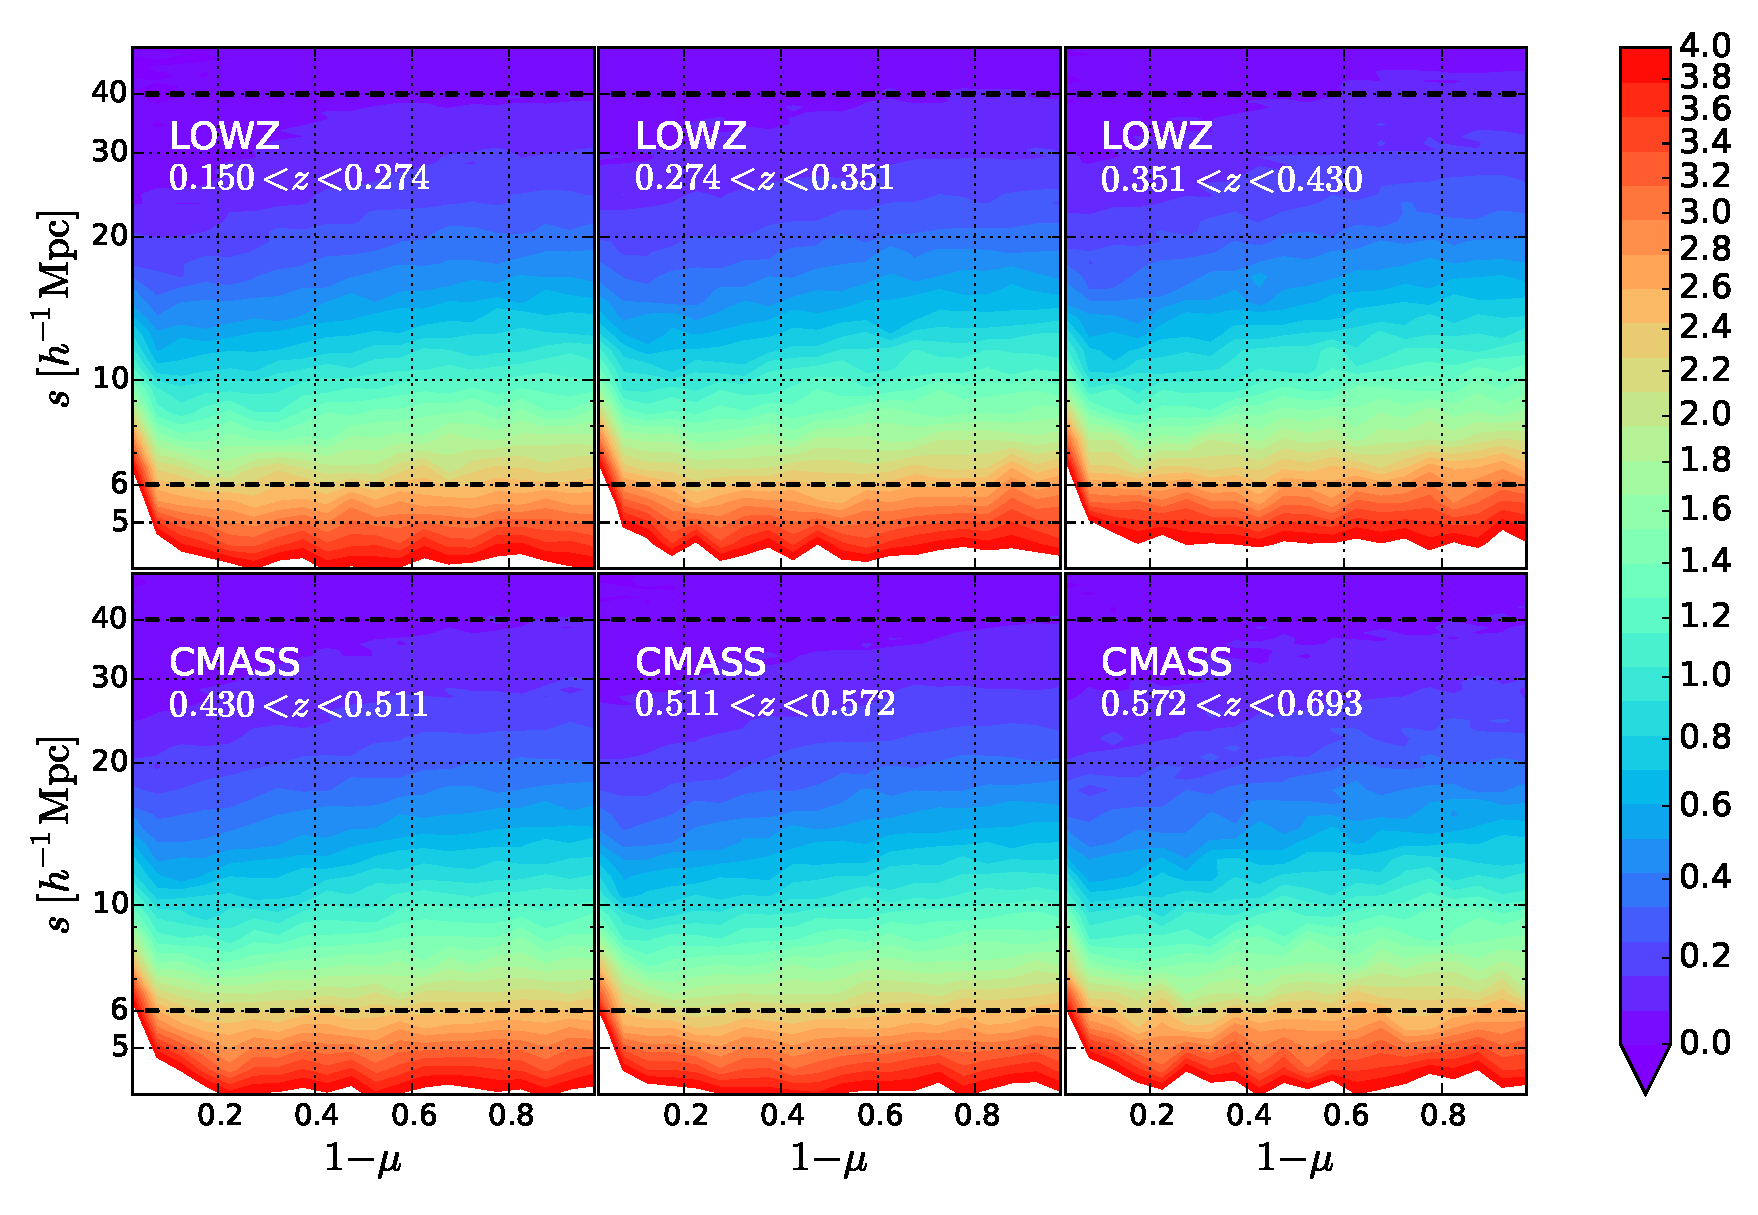
\includegraphics[width=14cm]{fig5.eps}
   %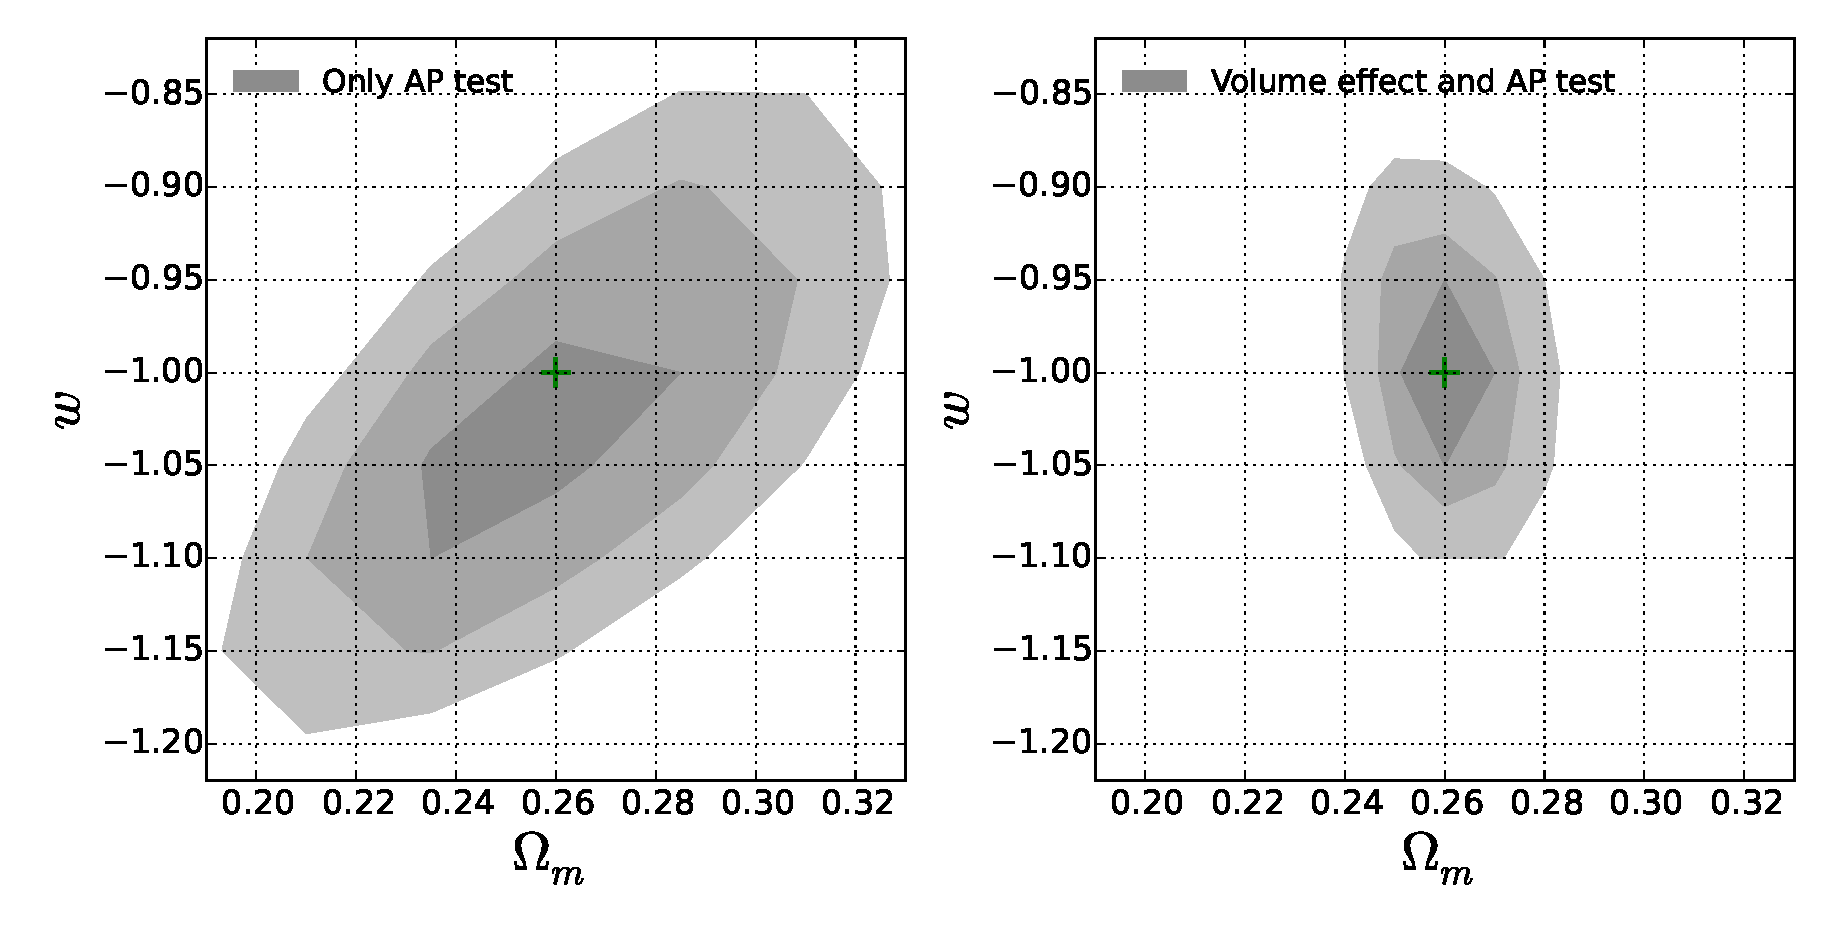
\includegraphics[width=14cm]{Tpcf--contour.eps}
   }
   \caption{
    \label{fig_2pcfcon} 
    2D contour map of measured $\xi$ as a function of $\mu$ and $s$, from the six redshift bins of LOWZ and CMASS samples 
      in the cosmology of $\Omega_m=0.31$ $\Lambda$CDM model.
    The black dashed lines mark the scales 6\ $h^{-1}$Mpc $\leq s\leq$ 40\ $h^{-1}$Mpc.
    %The correlation functions have rather large values on small sales such as $s=5$ $h^{-1}$Mpc,
    %  and monotonically decreases to smaller values on larger scales due to weaker clustering.
    The contour lines are not horizontal due to the effects of peculiar velocity.
    The FOG and Kaiser effects clearly manifest themselves through the tilting of contour 
     lines where $1-\mu \rightarrow 0$ and $1-\mu \gtrsim0.1$, respectively.
    The six contour maps have rather similar appearance, implying small redshift evolution of $\xi$.
   }
      %The redshift density distribution of the BOSS DR12 galaxy samples, assuming a $\Lambda$CDM cosmology with $\Omega_m=0.31$.
      %The blue and green solid histograms show the distribution of LOWZ and CMASS galaxies respectively. 
      %The vertical dashed lines define the 6 redshift bins that are used to cut the samples.   }
\end{figure*}

\subsection{Measuring the correlation function}

%We probe the Alcock-Paczynski effects using the 2pCF. 
%The 2pCF is a mature statistic in cosmology and its optimal estimation considers minimal variance 
%while dealing with complicated masks and selection functions. 
%The most commonly adopted formulation is that of the 
We adopt the Landy-Szalay estimator~\citep{1993ApJ...412...64L} to calculate the 2pCF,
\begin{equation}
\xi(s,\mu)=\frac{DD-2DR+RR}{RR}\ ,
\end{equation}
where $DD$ is the number of galaxy--galaxy pairs, 
$DR$ the number of galaxy-random pairs, 
and $RR$ is the number of random--random pairs, 
all separated by a distance defined by $s\pm\Delta s$ and $\mu\pm\Delta\mu$, 
where $s$ is the distance between the pair and $\mu=\cos(\theta)$, 
with $\theta$ being the angle between the line joining the pair of galaxies and the LOS direction to the target galaxy. 
This statistic captures the anisotropy of the clustering signal.

The random catalogue consists of unclustered points whose number density in redshift space mimics the radial selection function of the observational data. 
To reduce the statistical variance of the estimator we use 50 times as many random points as we have galaxies.
The galaxies and random points are weighted as described in Sec. \ref{sec:data}.

Figure \ref{fig_2pcfcon} shows the 2D contour of measured $\xi$ as a function of $\mu$ and $s$,
from the six redshift bins of LOWZ and CMASS samples 
in the cosmology of $\Omega_m=0.31$ $\Lambda$CDM model.
%The correlation functions have rather large values on small sales such as $s=5$ $h^{-1}$Mpc,
%and monotonically decrease to smaller values on larger scales due to weaker clustering.
Due to the peculiar velocity effect, the contour lines are not horizontal.
The FOG \citep{FOG} and Kaiser \citep{Kaiser1987} effects 
clearly manifest themselves through the tilting of contour lines in regions of $\mu \rightarrow 1$ and $1-\mu \gtrsim0.1$, respectively.
A visual inspection of the contour maps from the six redshift bins 
reveals that they all have a similar appearance,
implying small redshift evolution of $\xi$.

\subsection{Probing the anisotropy through 2pCF}

The 2pCF is measured as a function of the separation $s$ and the angular direction $\mu$.
To probe the anisotropy we are more interested in the dependence of the 2pCF on $\mu$.
We follow the procedure of \cite{Li2015} and integrate the $\xi$ over the interval $s_{\rm max} \leq s \leq s_{\rm min}$.
We evaluate
\begin{equation}\label{eq:xideltas}
\xi_{\Delta s} (\mu) \equiv \int_{s_{\rm min}}^{s_{\rm max}} \xi (s,\mu)\ ds.%,\ \ \ {\rm at\ particular\ binned\ direction\ }\mu_i
\end{equation}
The integration is limited at both small and large scales.
At small scales the value of $\xi$ is seriously affected by the FOG effect \citep{FOG}
which depends on the galaxies bias.
This may introduce a redshift evolution in $\xi_{\Delta s}(\mu)$ that is relatively difficult to model.
At large scales the measurement is dominated by noise due to poor statistics.
\cite{Li2015} found that $s_{\rm min}=6-10$ $h^{-1}$Mpc and $s_{\rm max}=40-70$ $h^{-1}$Mpc are reasonable choices 
which provide consistent, tight and unbiased constraints on cosmological parameters.
In this analysis we choose $s_{\rm min}=6$ $h^{-1}$Mpc and $s_{\rm max}=40$ $h^{-1}$Mpc.

The redshift evolution of the bias of observed galaxies leads to redshift evolution of the strength of clustering,
which is difficult to accurately model.
To mitigate this systematic uncertainty we rely on the shape of $\xi_{\Delta s}(\mu)$, rather than its amplitude,
\begin{equation}\label{eq:norm}
 \hat\xi_{\Delta s}(\mu) \equiv \frac{\xi_{\Delta s}(\mu)}{\int_{0}^{\mu_{\rm max}}\xi_{\Delta s}(\mu)\ d\mu}.
\end{equation}
We impose a cut $\mu<\mu_{\rm max}$ to reduce the fiber collision and FOG effects which are stronger toward the LOS ($\mu\rightarrow1$) direction.

\begin{figure*}
   \centering{
   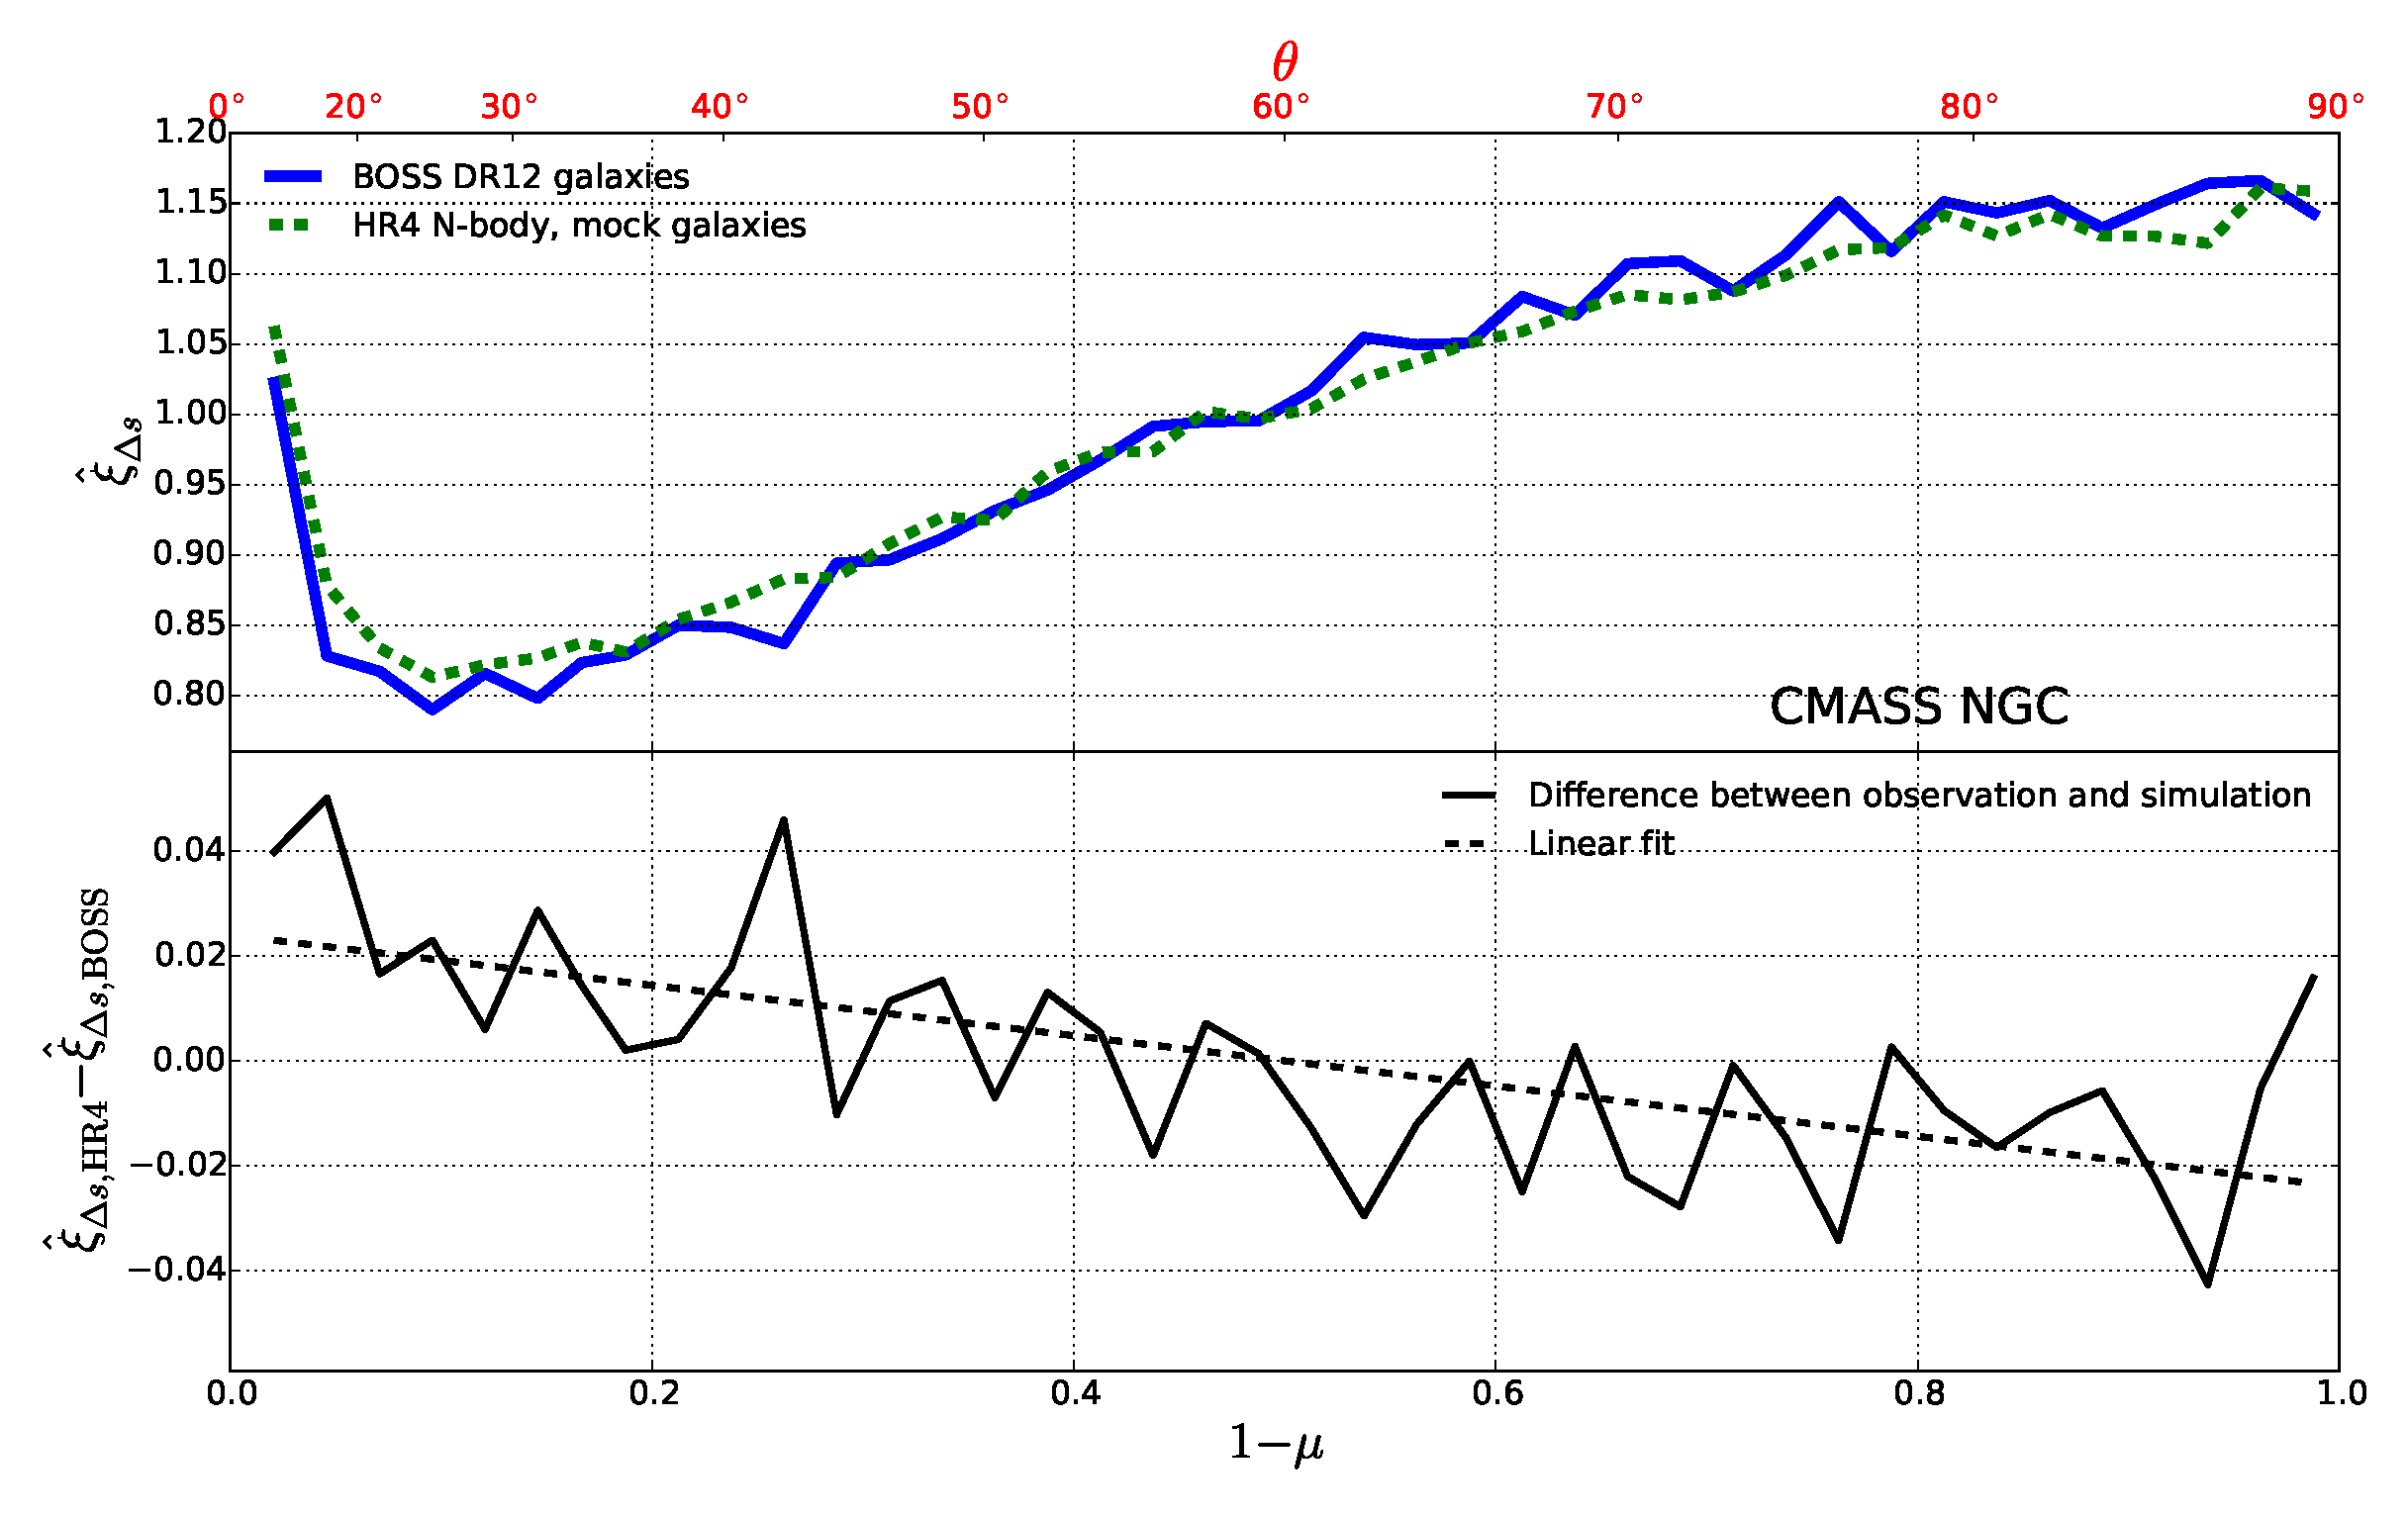
\includegraphics[width=16cm]{fig6.eps}
   }
   \caption{\label{fig_datamock}
   %Apparent distortion of objects in four wrongly assumed cosmologies, assuming a true cosmology of .
   $\hat\xi_{\Delta s}(\mu)$ measured from BOSS DR12 CMASS NGC sample 
    (consists of $\approx 565\,000$ galaxies at $0.15 < z < 0.693$)
    and one realization from the HR4 N-body simulation, in the WMAP5 cosmology.
   The lower panel shows the difference between the results of observational data and mock galaxies.
   $\hat\xi_{\Delta s}(\mu)$ are obtained by integrating $\xi (s,\mu)$ within the range {\rm 6\ $h^{-1}$Mpc}$\leq s\leq${\rm 40\ $h^{-1}$Mpc} 
      and normalizing the amplitude, 
    i.e., Eq. (\ref{eq:xideltas}) and Eq. (\ref{eq:norm}).
   To produce a clear view of the FOG effect, we split the angular range of $0.01\leq \mu \leq 1$ into as many as 40 bins.
   Using the HR4 mock galaxies, the enhancement near $\theta=0^\circ$ caused by the FOG effect
    and the tilt of the shape in $20^\circ\lesssim\theta\lesssim90^\circ$ 
    as a result of the large-scale flow,
    are all very well reproduced.
%    Thw lo
   This verifies the ability of our galaxies assignment method \citep{hong2016} 
    to reproduce the properties of galaxy distributions from large scale surveys.
   %Conversely, the HR3 PSB halo mock can not 
   %reproduce the shape of $\hat\xi_{\Delta s}(\mu)$.
   We use the HR4 mock galaxies to correct the systematics effects produced by the RSD.
   %The 72 sets of PSB mocks from HR3 are used to compute covariance.
   %measured by an observer located at the origin.
   %For reference, blue dashed squares show their shapes and positions in the true cosmology.
   }
\end{figure*}


The clustering properties may be affected by various properties of the galaxy sample, 
such as, for example the mass, morphology, color, concentration. 
In our simulation, using the merger tree, 
we identify ``galaxies'', therefore we only use the galaxy mass building history to simulate BOSS galaxies. 
Therefore, it is necessary for us to test if our mock galaxies can accurately 
reproduce the $\hat\xi_{\Delta s}(\mu)$ of observed galaxies.

%The clustering properties may be affected by the redshift evolution of properties of the galaxy sample, 
%such as the mass, morphology, color, concentration, and so on. 
%In our simulation, using the merger tree, we identify 'galaxies' so that we only use the galaxy mass to simulate BOSS galaxies. Therefore, it was necessary for us to test if our mock galaxies can accurately reproduce the shape of $\xi_{\Delta s}(\mu)$ of observed galaxies.

%As shown by Figure 6, the mock galaxies from our HR4 simulation can well reproduce the 
%$\hat\xi_{\Delta s}(\mu)$ of the observed galaxies.
Figure \ref{fig_datamock}  compares the shape of $\hat\xi_{\Delta s}(\mu)$ measured from observational data and mock survey samples.
It is clear that $\hat \xi_{\Delta s}(\mu)$ from mock galaxies identified in the HR4 simulation (green dotted line) agrees well with the observation.
%The HR4 galaxy mock can well reproduce the result from observational measurement.
The enhancement near $\theta=0^\circ$ is caused by the FOG effect,
and the characteristic shape in $20^\circ\lesssim\theta\lesssim90^\circ$ 
produced from the large-scale flow
are all very well reproduced.
This result verifies the ability of our mock galaxies to reproduce the clustering properties of the observed galaxies.
The small overestimate (underestimate) of $\hat\xi_{\Delta s}$ at large (small) $\mu$ could be due to 
that our mocks galaxies are more massive than those in the observations.
%methodology. (AMTB: need some good expression; need consult SW)
%Conversely, the HR3 PSB halo galaxies do not accurately reproduce the observations.
We use the HR4 galaxy mocks to correct the systematics.
%The HR3 PSB mock galaxies are used to estimate the covariance of 2pCF since 72 mock survey samples are available.

\begin{figure*}
   \centering{
   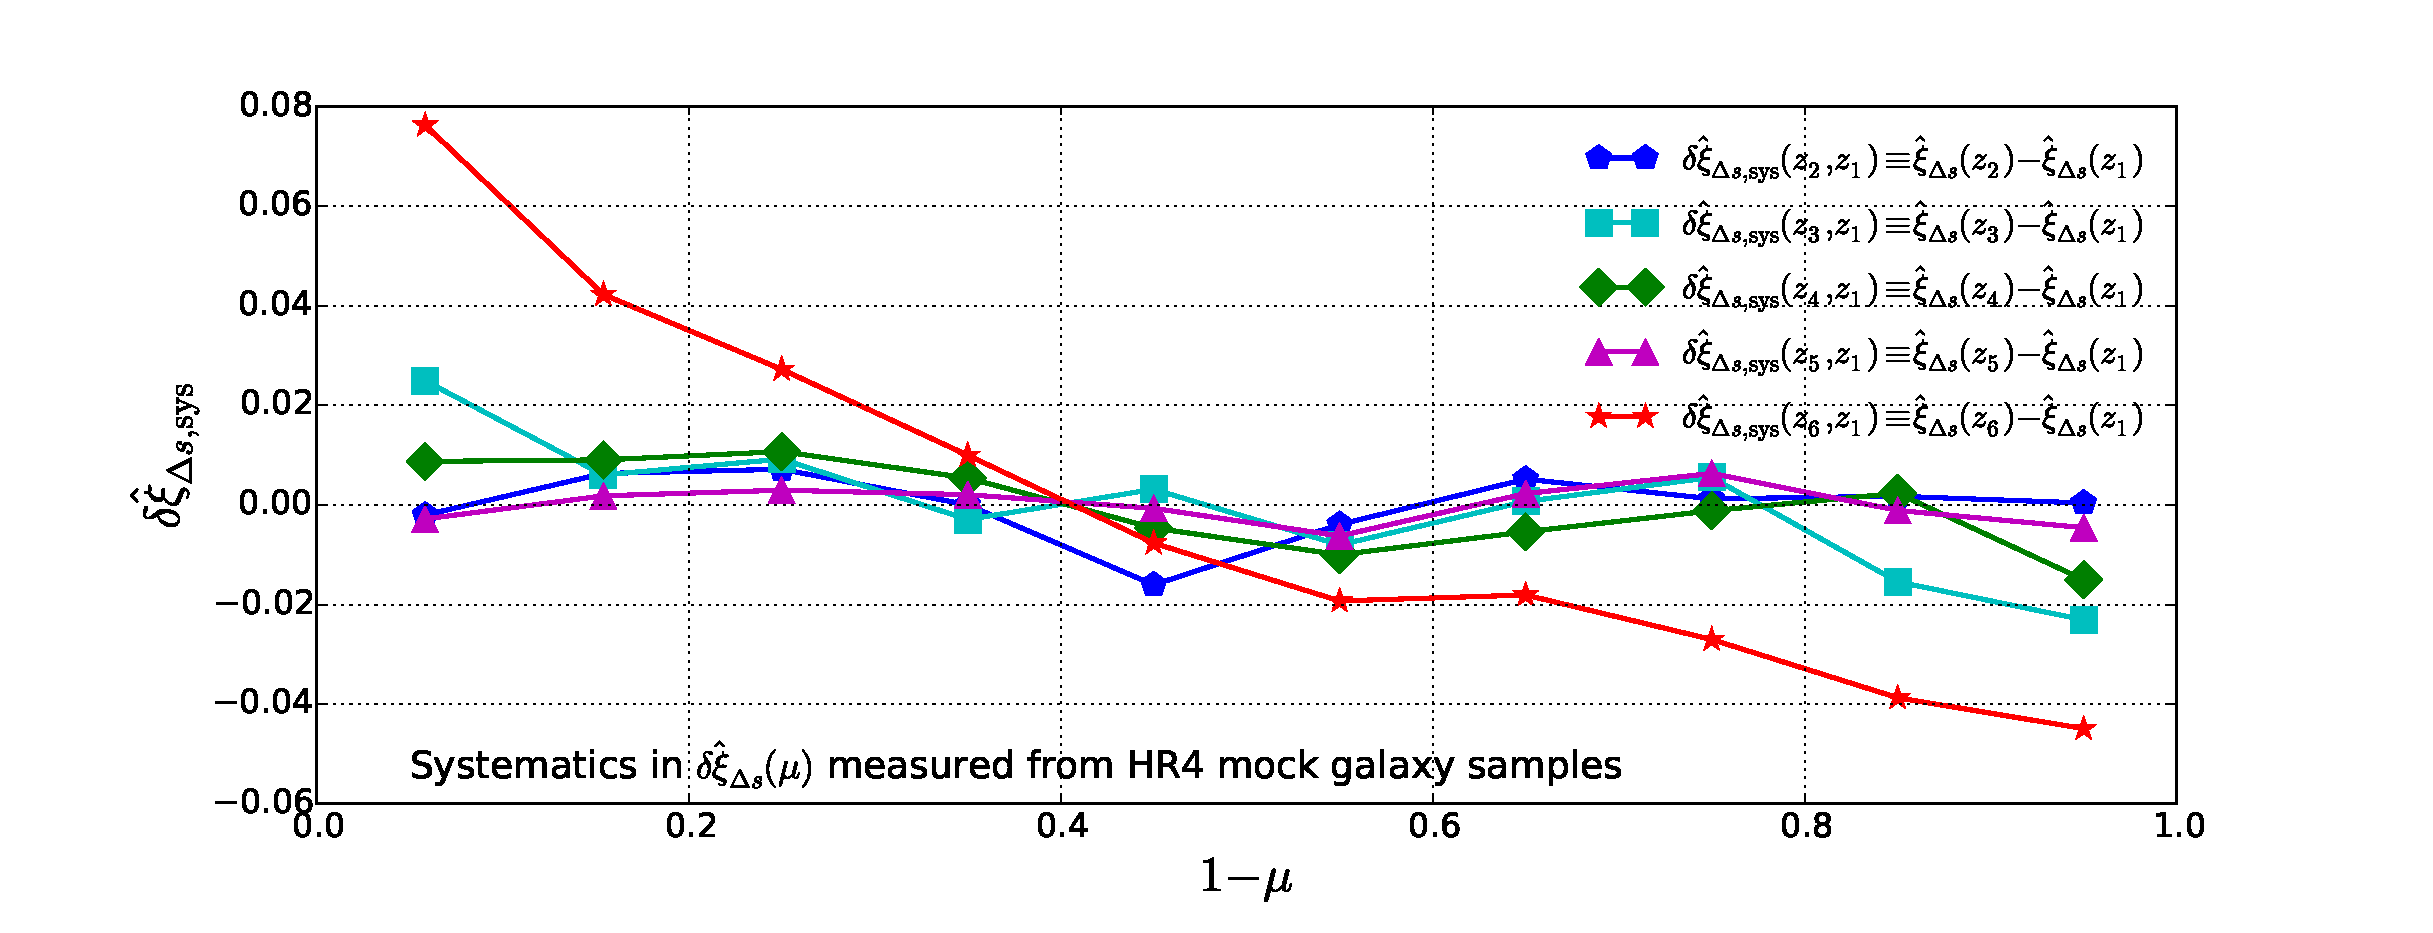
\includegraphics[width=16cm]{fig7.eps}
   %\includegraphics[height=9cm]{Tpcf-sys.eps}
   }
   \caption{\label{fig_sys}
   %Apparent distortion of objects in four wrongly assumed cosmologies, assuming a true cosmology of .
   Systematics in $\delta \hat \xi_{\Delta s}$, measured from the HR4 mock galaxy samples.
   The redshift evolution of RSD effect and properties of samples can lead to non-zero values of $\delta \hat\xi_{\Delta s}(z_i,z_1)$.
   For the 1st to 5th redshift bins, $\delta\hat\xi_{\Delta s, \rm sys}(z_i,z_1)\lesssim0.02$,
    indicating a small redshift evolution of the RSD effect and properties of galaxies.
   For the 6th redshift bin, the values of $\delta\hat\xi_{\Delta s, \rm sys}(z_6,z_1)$ are relatively large,
   because galaxies in that highest redshift bin are significantly more massive than those at lower redshifts.
   % so the measured $\hat\xi_{\Delta s}(\mu)$ has larger (smaller) values at $\mu\rightarrow1$ ($\mu\rightarrow0$) 
   % compared with the others.
   See Sec. \ref{sec:syscor} for details.
   %The values are estimated from the HR4 mock galaxies. % and subtract its contribution.
   }
\end{figure*}


%It is impossible to probe $\hat\xi_{\Delta s}(\mu)$ as a continuous function with infinite degrees of freedom. 
We divide the full angular range $0\leq\mu\leq\mu_{\rm max}$ into $n_{\mu}$ bins and measure its value in each bin.
Since we are free to choose $\mu_{\rm max}$ and $n_{\mu}$,
they are varied to optimize the S/N of our results.
This topic will be discussed in Sec. \ref{sec:binningscheme}.

\subsection{Characterizing the redshift evolution}


As shown in Figure \ref{fig_nbar}, we split the BOSS DR12 galaxies into six redshift bins, three in LOWZ and three in CMASS.
To study the redshift evolution of the clustering anisotropy 
we use the {\it first redshift bin} as the reference and compare the measurements in other bins with that in the first.
We define
\begin{equation} \label{eq:deltahatxi}
\delta \hat\xi_{\Delta s}(z_i,z_1,\mu_j)\ \equiv\ \hat\xi_{\Delta s}(z_i,\mu_j) - \hat\xi_{\Delta s}(z_1,\mu_j)
\end{equation}
where $\hat\xi_{\Delta s}(z_i,\mu_j)$ is $\hat\xi_{\Delta s}$ measured in the $i$th redshift bin and $j$th $\mu$ bin,
where $1\leq i \leq 6$ and $1\leq j \leq n_{\mu}$.
To characterize the shape of the curve well $n_\mu \gtrsim5$ is required.

\subsection{Correction for systematics}\label{sec:syscor}

Other than the AP effect, there are additional effects 
which may produce redshift-dependent anisotropy and affect the results. 

The observational artifacts, such as fiber collisions, redshift failures, 
and the non-cosmological density fluctuations with stellar density and seeing,
are accounted for in the galaxy weights \citep{Reidetal:2016}.
Fiber collisions and redshift failures may affect the value of $\hat\xi(\mu)$ in the region close to LOS;
%We correct them by reweighting galaxies, include fiber collisions in the construction of mock surveys,
we abandon the angular region of $1-\mu<0.01$, 
to avoid possible systematics (see Appendix \ref{sec:RBtest} for more discussion). 

%The SGC catalogues have higher target density than NGC and 
%thus a higher galaxy number density, known as the north/south asymmetry.
The non-contiguous NGC and SGC are less well cross-calibrated with respect to each other 
than they are internally calibrated \citep{Schlafly2010,SF2011,Parejko2013}.
We construct the NGC and SGC mock surveys separately to avoid possible systematics.
The 2pCF analysis is also carried out for the NGC and SGC independently.
%Also, in this analysis we only look at the radial evolution of clustering properties. 
The result should be robust as long as each catalogue is well calibrated internally.


%The variation in the density of catalogues is not expected to have large effect on our analysis.

%The redshift evolution of AP effect, RSD effect and properties of samples all may lead to non-zero values of $\delta \hat\xi_{\Delta s}$.
%To measure the signal from the redshift evolution of the AP effect,
%we estimate the value of $\delta \hat\xi_{\Delta s}$ from the other effects and subtract their contribution
%(hereafter $\delta\hat\xi_{\Delta s, \rm sys}$) from the total variation.

The apparent anisotropy introduced by RSD is, 
although greatly reduced by focusing on the redshift evolution, 
still the most significant systematic effect.

We estimate the value of $\delta \hat\xi_{\Delta s}$ from the systematic effects and subtract their contribution
(hereafter $\delta\hat\xi_{\Delta s, \rm sys}$) from the total variation.
The quantity $\delta\hat\xi_{\Delta s, \rm sys}$ is estimated from the HR4 mock galaxies.
The mock survey sample imitates the SDSS BOSS sample by mimicking
the survey as close as possible and includes past light cone effects.
The observational systematics such as the RSD, survey geometry, and shot noise
are included in the exactly same way as the observation.
The peculiar velocity perturbs the observed redshift through the relation
\begin{equation}\label{eq:zvpeu}
\Delta z = (1+z) \frac{v_{{\rm LOS}}}{c},
\end{equation}
where $v_{\rm LOS}$ is the LOS component of the peculiar velocity of galaxies.
The redshift evolution of galaxy peculiar velocities, 
resulting from growth of structure,
causes the anisotropy produced by RSD to have a small redshift evolution; 
this is the main source of systematic uncertainty in our results. 

We take the HR4 mock galaxy samples and compute $r(z)$ of galaxies in the cosmology under which the simulation is based.
In this case there is no AP effect. 
Thus, the measured $\delta \hat\xi_{\Delta s}$ are the redshift evolution purely created by systematics effects.
They are adopted as the estimation of $\delta\hat\xi_{\Delta s, \rm sys}$,
and the results are illustrated in Figure \ref{fig_sys}. %shows $\delta\hat\xi_{\Delta s, \rm sys}(z_i,z_1)$ measured from the HR4 mock galaxy samples.
%Measurements of $\hat\xi_{\Delta s}$ in the 2th to 6th redshift bins are compared with that in the first bin.

For the 1st to 5th redshift bins, $\delta\hat\xi_{\Delta s, \rm sys}(z_i,z_1)\lesssim0.02$,
indicating a small redshift evolution of the RSD effect and properties of galaxies.
The only exception is the 6th redshift bin where the values of $\delta\hat\xi_{\Delta s, \rm sys}(z_6,z_1)$ are relatively large.
The reason for the large values is that the galaxies in that highest redshift bin are significantly more massive than those at lower redshifts,
so the measured high redshift $\hat\xi_{\Delta s}(\mu)$ has larger (smaller) values at $\mu\rightarrow1$ ($\mu\rightarrow0$) 
compared with the others
(an investigation of the dependence of $\hat\xi_{\Delta s}(\mu)$ on galaxy mass is provided in Sec. \ref{sec:caveats}).

%This should be the reason why .


\subsection{The caveats}\label{sec:caveats}

%The biggest systematic of our method, like all other applications of AP, is still the RSD problem.
\cite{Li2014,Li2015} found the RSD effect exhibits a small redshift dependence of $\hat \xi_{\Delta s}(\mu)$, 
mainly due to the structure growth and the selection effect
(different galaxy bias at different redshifts).
In this analysis we use the mock galaxy sample from HR4 to correct this systematics.
The galaxy assignment scheme of \cite{hong2016} applied to HR4 is very successful in modeling both the 
large scale Kaiser effect and the small scale FOG effect in nonlinear regions.
%After correcting the systematic effect of RSD, we obtain reasonable cosmological constraint consistent with all other cosmological probes.

There are two possible caveats in our procedure of the modeling of the RSD effect.

1) The RSD effect is estimated from mock survey samples created in a particular cosmology, 
i.e., the $\Omega_m=0.26$ $\Lambda$CDM model. %model from WMAP5 observations with .
If this adopted cosmology is different from the truth, then there could be a systematic bias in the estimation. %of RSD
We believe that this will not seriously affect our cosmological constraints.
\cite{Li2014} shows that the redshift dependence of RSD is not sensitive to cosmological parameters.
Also, the cosmologies adopted in the HR3 and HR4 simulations are consistent with our best-fit cosmological parameters within 1$\sigma$,
therefore our inferred cosmological constraints should be fairly accurate.
In a future analysis,
we will estimate the redshift evolution of the RSD effect from a set of cosmological simulations 
covering the relevant part of the parameter space.
This approach will remove the remaining uncertainty associated with the RSD effect, 
which is already a minor effect in our analysis.
%the statistical uncertainty of this method could be much smaller,
%and modeling the RSD effect in a cosmological dependent manner would be necessary.

\begin{figure*}
   \centering{
   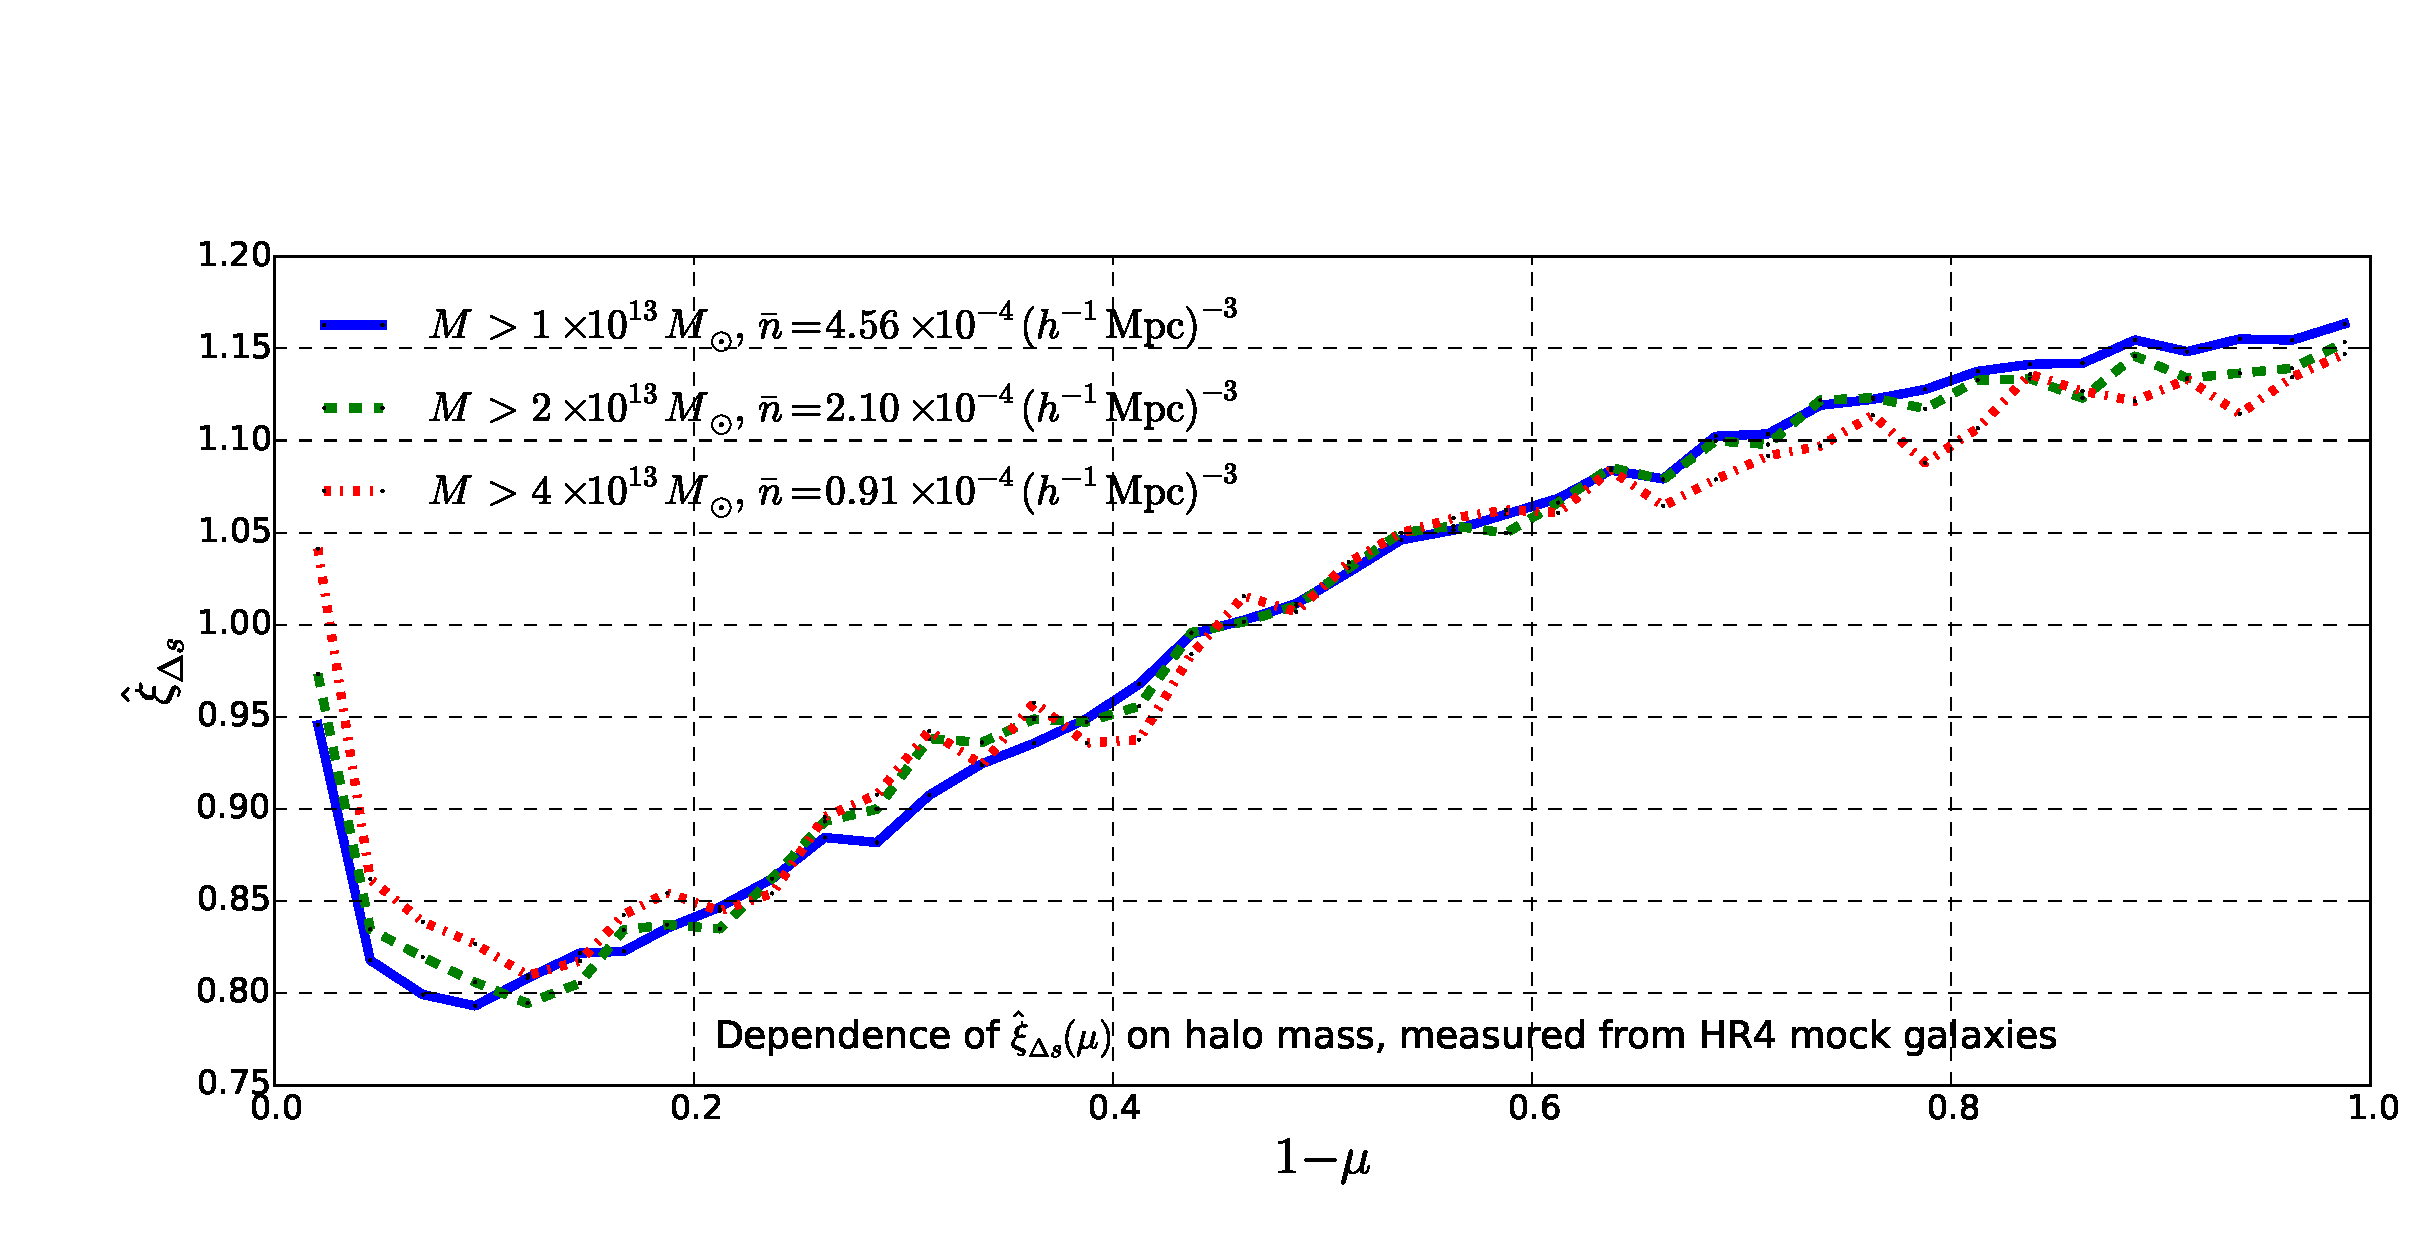
\includegraphics[width=14cm]{fig8.eps}
   %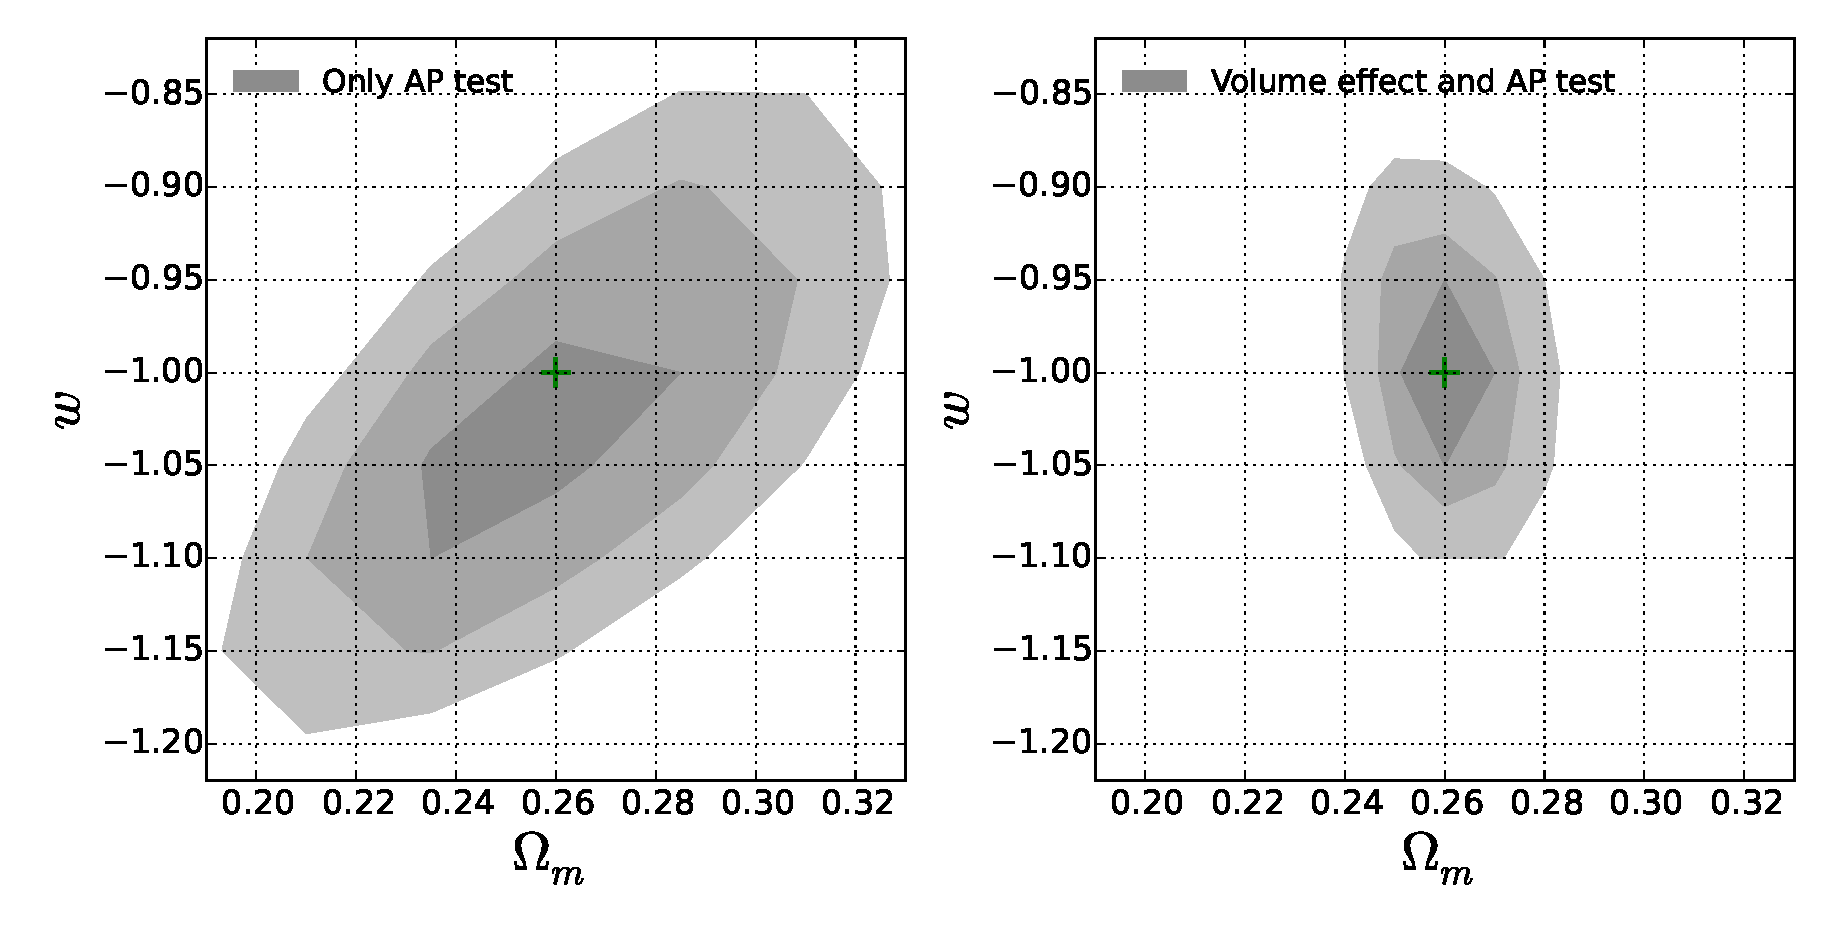
\includegraphics[width=14cm]{Tpcf--contour.eps}
   }
   \caption{
    \label{fig_2pcf_masscut} 
    $\hat \xi_{\Delta s}(\mu)$ measured from a small HR4 mock galaxy sample with different minimal mass cuts.
    The mock galaxies are taken from the $z=0$ snapshot data within the radius $r<600$ $h^{-1}$Mpc.
    Only small variations of $\hat\xi_{\Delta s}(\mu)$ are produced when changing the minimal mass cuts.
    Higher mass cuts result in larger (smaller) $\hat\xi_{\Delta s}(\mu)$ at $\mu\rightarrow1$ ($\mu\rightarrow0$).
    Considering the large variation of mass cuts, the variation of $\hat\xi_{\Delta s}(\mu)$ is not significant.
   }
      %The redshift density distribution of the BOSS DR12 galaxy samples, assuming a $\Lambda$CDM cosmology with $\Omega_m=0.31$.
      %The blue and green solid histograms show the distribution of LOWZ and CMASS galaxies respectively. 
      %The vertical dashed lines define the 6 redshift bins that are used to cut the samples.   }
\end{figure*}

2) The selection effect, i.e., the evolution of galaxy bias with redshifts, 
can introduce redshift evolution in the clustering properties of the observed galaxies.
%If that is not accurately modeled, people may worry about systematics. %may suffer from systematic errors.
%Again, we believe this is not a serious problem for our analysis.
In our analysis the amplitude of the 2pCF is normalized and only its angular information, 
the function $\hat \xi_{\Delta s}(\mu)$, is used.
This function is rather insensitive to the galaxy bias,
which mainly affects the strength of clustering.

As a test, Figure \ref{fig_2pcf_masscut} shows $\hat \xi_{\Delta s}(\mu)$ measured from a small HR4 galaxy sample with different minimal mass cuts.
The mock galaxies are taken from the $z=0$ snapshot data within the radius $r<600$ $h^{-1}$Mpc.
Applying the minimal mass cuts of $1,2,4\times 10^{13} h^{-1} M_{\odot}$, 
we created three sets of subsamples with number density of 
$\bar n=4.56,\ 2.10,\ 0.91 \times 10^{-4} ( h^{-1} \rm Mpc)^{-3}$, 
which roughly covers the scatter of the number density of BOSS DR12 galaxies at $0.15<z<0.7$
\footnote{The BOSS LOWZ and CMASS galaxies reside in massive haloes 
with a mean halo mass of $5.2 \times 10^{13} h^{-1} M_{\odot}$ and $2.6 \times 10^{13} h^{-1} M_{\odot}$ \citep{Parejko2013,White2011,Reidetal:2016},
respectively.
For CMASS galaxies, when the redshift changes from $z=0.43$ to $0.7$,
the mean stellar mass varies from $10^{11.6} {M_{\odot}}$ to $10^{11.9} {M_{\odot}}$ \citep{CMASSLSS2014}.}.



For subsamples with higher mass cuts the $\hat\xi_{\Delta s}(\mu)$
has larger (smaller) values at $\mu\rightarrow1$ ($\mu\rightarrow0$).
More massive samples result in less tilted $\hat\xi_{\Delta s}(\mu)$ in the region of $1-\mu\gtrsim0.1$
\footnote{This phenomenon is understandable.
The tilt of $\hat\xi_{\Delta s}(\mu)$ is related to the RSD effect, 
and also the overall amplitude of the 2pCF (the denominator of Eq. (\ref{eq:norm})).
The slope should be roughly proportional to $(v/b_g)^2$, 
where the peculiar velocity term $v^2$ denotes the effect of RSD, 
and the galaxy bias term $b_g^2$ represents the amplitude of the 2pCF. 
For the more massive sample, $b_g$ is much larger while $v$ is still close to the peculiar velocity of dark matter field,
%So their curves are less tilted.
therefore the slope is smaller.
}.
This explains the relative large value of $\hat \xi_{\Delta s,\rm sys}(z_6, z_1)$.
In particular, comparing the subsamples with mass cuts $4\times 10^{13}h^{-1} M_{\odot}$ and $1\times 10^{13}h^{-1} M_{\odot}$, 
we find the red dotted curve is higher (lower) than the blue solid line at $\mu\rightarrow1$ ($\mu\rightarrow0$),
with a difference of $\approx$0.1 (0.05),
consistent with the value of $\hat \xi_{\Delta s,\rm sys}(z_6, z_1)$ shown in Figure \ref{fig_sys}.

In addition, this result also explains the small discrepancy between the $\hat\xi_{\Delta s}(\mu)$ measured from the 
observational data and the HR4 simulations (Figure \ref{fig_datamock}).
The mock galaxies could be systematically more massive than the observed ones.
These systematics could be most significant in the 6th redshift bin
where mock galaxies are most massive, 
leading to possible overestimation of $\delta\hat\xi_{\Delta s,{\rm sys}}$.
We discuss the impact of this effect in Sec. 6.1.

Considering the large variation of mass cuts, the change of $\hat\xi_{\Delta s}(\mu)$ is not significant,
so we conclude that $\hat\xi_{\Delta s}(\mu)$ is relatively insensitive to the galaxy bias.



%In addition, Figure 5 of \cite{Li2015} also shows that the peculiar velocities of the halos (PSB halos from HR3) are very insensitive to their masses. 
%This means the RSD effect coming from galaxies with different biases are similar.
%So the modeling of RSD effect does not require accurate modeling of the biases of the observed galaxies.

\subsection{$\chi^2$ function}\label{sec:likelihood}

We define a $\chi^2$ function to quantify the redshift evolution of clustering anisotropy
\begin{equation}\label{eq:chisq1}
\chi^2\equiv \sum_{i=2}^{6} \sum_{j_1=1}^{n_{\mu}} \sum_{j_2=1}^{n_{\mu}} {\bf p}(z_i,\mu_{j_1}) ({\bf Cov}_{i}^{-1})_{j_1,j_2}  {\bf p}(z_i,\mu_{j_2}),
\end{equation}
where ${\bf p}(z_i,\mu_{j})$ is the redshift evolution of clustering, 
$\hat \xi_{\Delta s}$, with systematic effects subtracted
\begin{eqnarray}\label{eq:bfp}
 {\bf p}(z_i,\mu_{j}) \equiv&\ \delta \hat\xi_{\Delta s}(z_i,z_1,\mu_j) - \delta \hat\xi_{\Delta s, \rm sys}(z_i,z_1,\mu_j)
\end{eqnarray}
${\bf Cov}_i$ is the covariance matrix estimated from the 72 sets of PSB mock galaxies identified from HR3 N-body simulation.

\subsection{Averaging a set of replicate measurements to increase the S/N}\label{sec:binningscheme}

The angular cut, $\mu_{\rm max}$, and number of bins, $n_\mu$, is chosen freely.
%The cut $\mu_{\rm max}$ and the number of bins $n_\mu$ can be chosen freely in our analysis.
Different choices for these parameters yield slightly different results and different statistical uncertainties.
To suppress the statistical noise we adopt a large number of binning schemes and average their $\chi^2$s.

A value $\mu_{\rm max} = 0.99$ is sufficient to remove the fiber collision effect.
We have checked that our results are statistically robust against the choice of $\mu_{\rm max}$.

A larger $n_\mu$ tightens the constraint 
in the cost of more noise, 
while $n_\mu$ should be smaller than the number of mock samples used for covariance estimation.
We find $n_\mu \gtrsim 5$ gives relative tight constraints, 
and $n_\mu = 40$ is the limit we can reach given the size of the sample and the number of mock samples.

We run through the range $\mu_{\rm max} = 0.85, 0.86, ... 0.99$ at steps of 0.01 and $n_\mu = 5, 6, ... 40$, in total 540 binning schemes.
%\footnote{In fact we only use 381 schemes.
%In some cases the estimation of covariance is not very successful, leading to singular matrix or very noisy $\chi^2$;
%We reject these cases.}.
We compute $\chi^2$ according to Equation (\ref{eq:chisq1}) for these choices and take an average of these $\chi^2$s.
This approach suppresses the statistical noise quite effectively. %in the contour map of $\chi^2(\Omega_m,w)$.



%We find noise in the $\chi^2$ probably due to the low statistic caused by the limited size of the sample and the covmat due to small size of mocks ...
%So we compute many values of $\chi^2$ using different $n_\mu$ and $\mu_{\rm max}$...
%The noise in $\chi^2$ shall be statistically random and by taking an average it is suppressed while the physical signal is preserved...
%We tested the dependence of the result on $\mu_{\rm max}$ and find the result is rather stable within the range $\mu_{\rm max}=0.85 - 0.99$...
%So we use $\mu_{\rm max} = 0.85, 0.86, ... 0.99$...
%Increasing $n_\mu$ tighens the constraintm, but in cost of larger noise in the result...
%Also $n_\mu$ shall be smaller than the number of mocks to compute covmat...
%So we use $n_\mu = 5, 6, ... 40$...
%So we define...
%\begin{equation}\label{eq:chisq2}
%\bar\chi^2\equiv \frac{ \sum \chi^2(n_\mu,\ \mu_{\rm max}) } {\rm Number\ of\ \chi^2} ... (find a proper way to illustrate this equation)
%\end{equation}

%{\bf AMTB: We need to give some results on the systematic effects. }



\begin{figure*}
   \centering{
   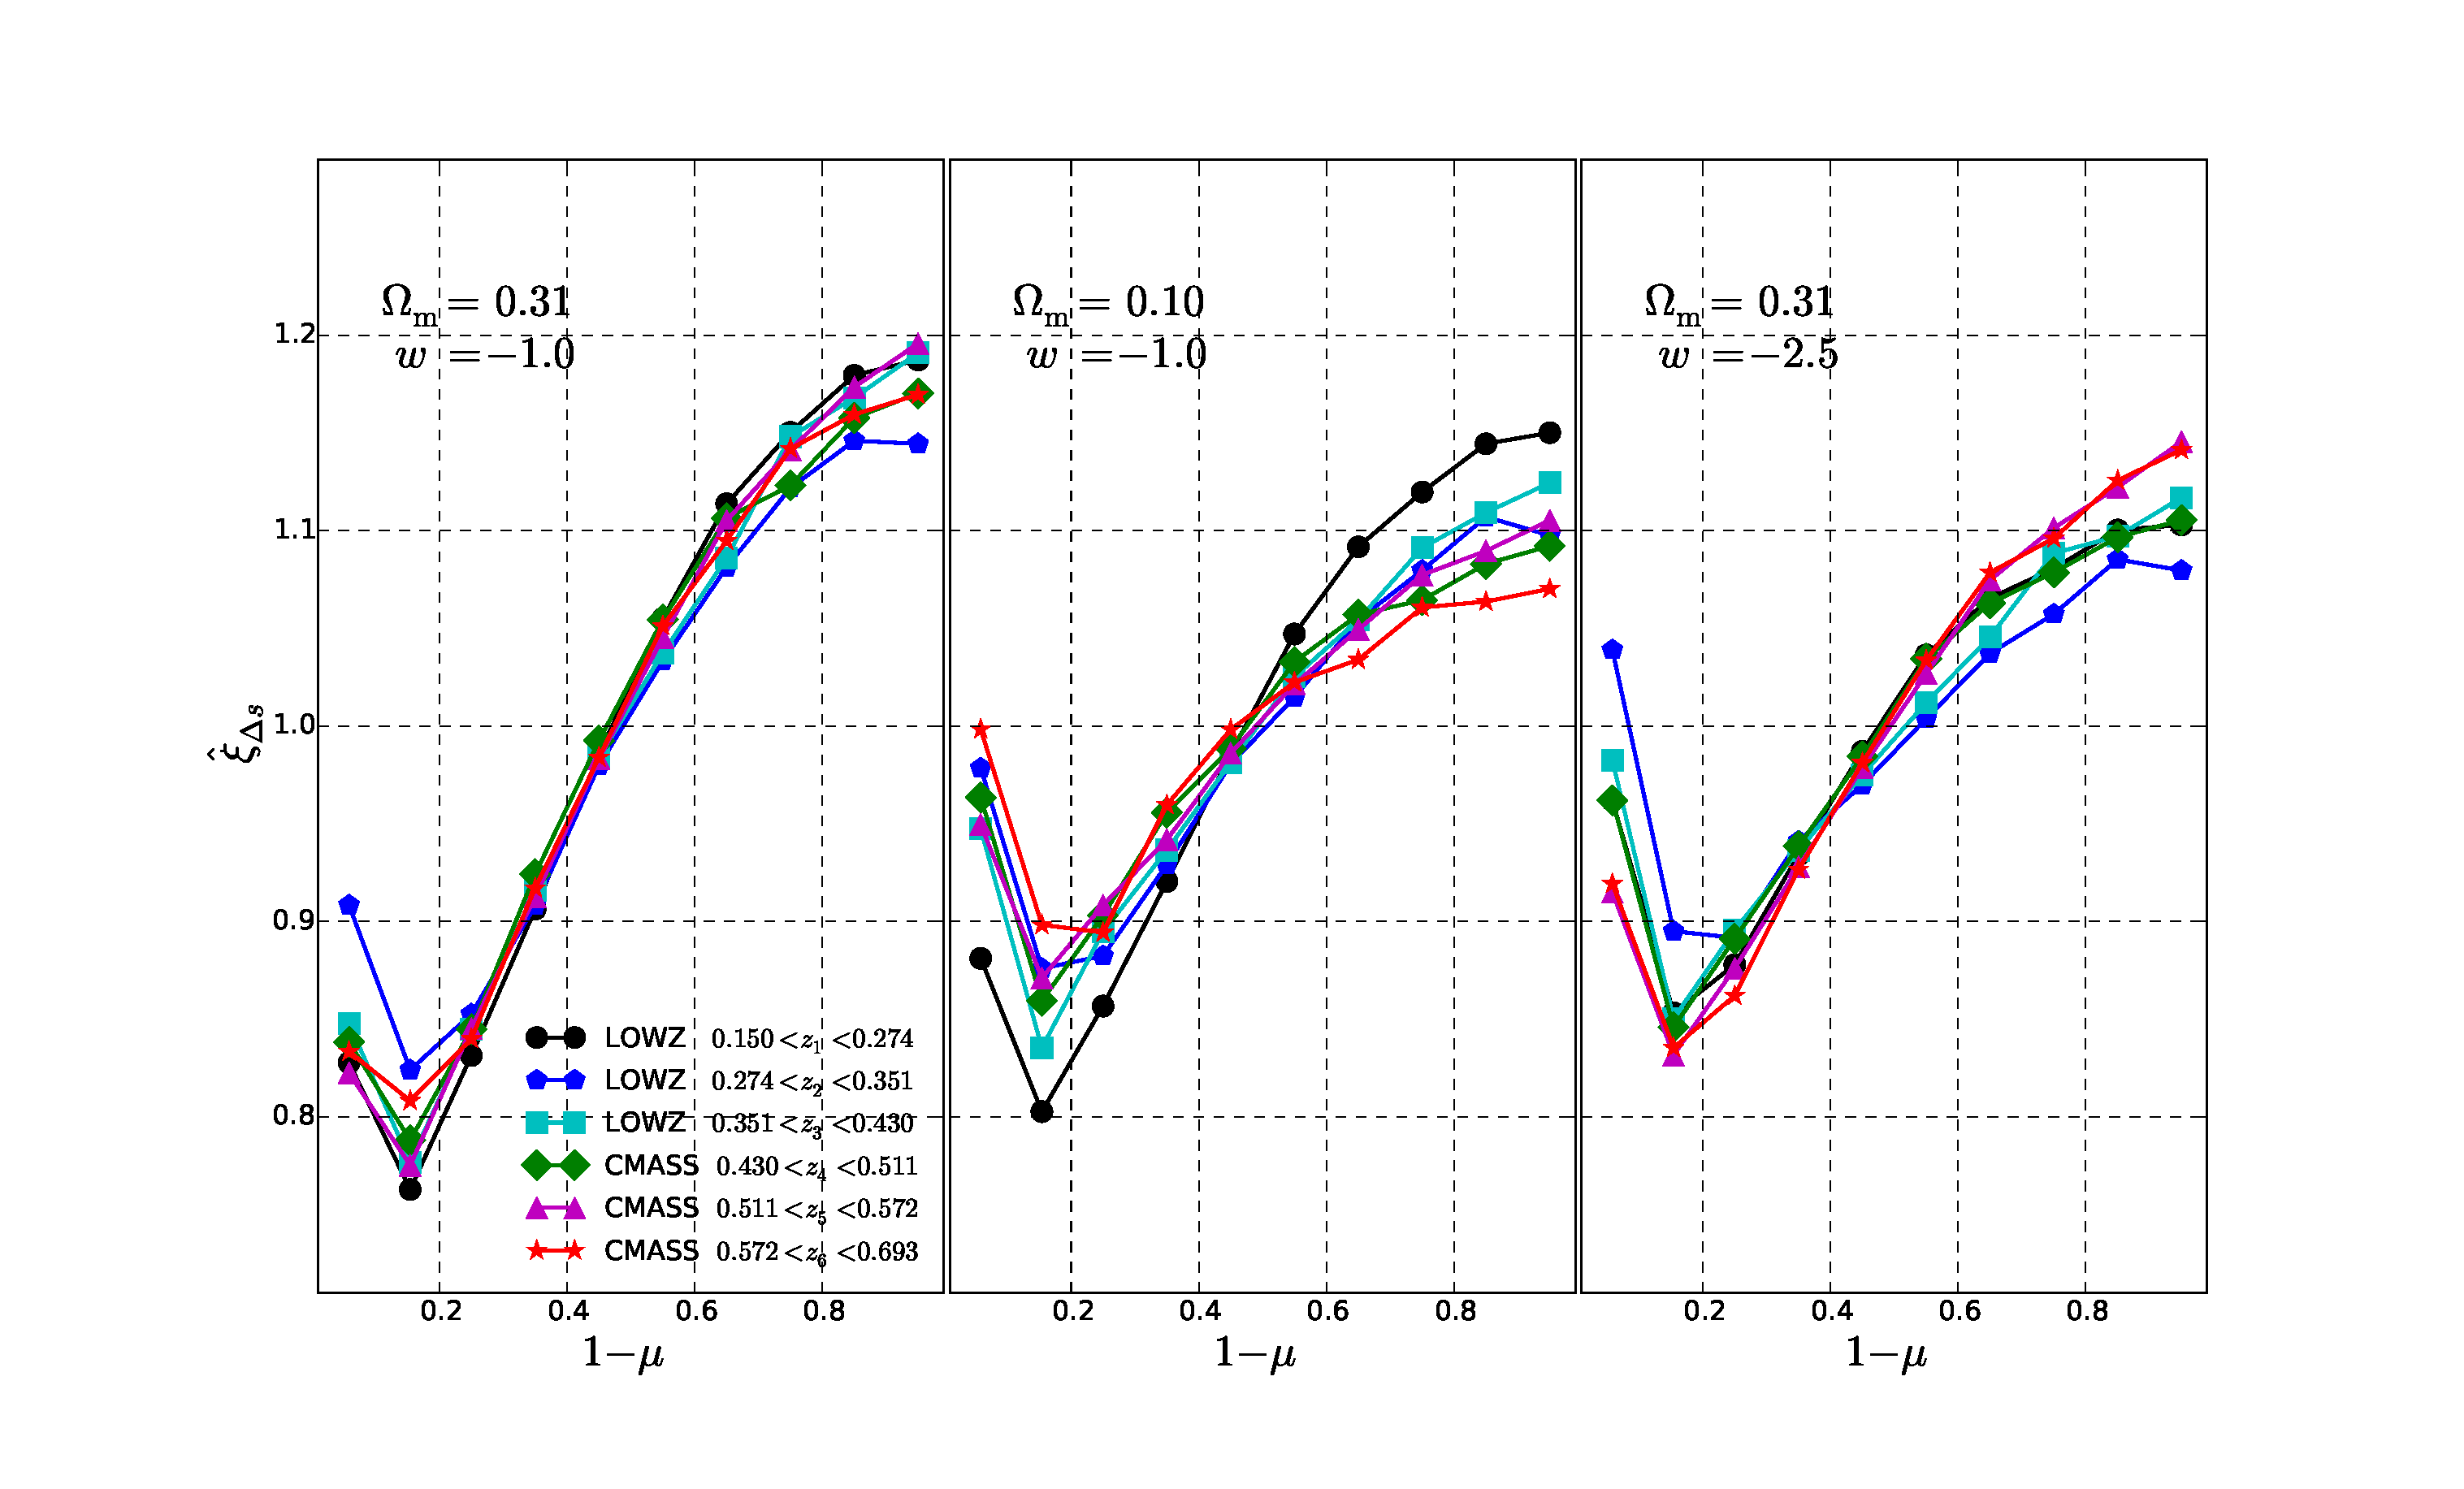
\includegraphics[width=18cm]{fig9_0.eps}
   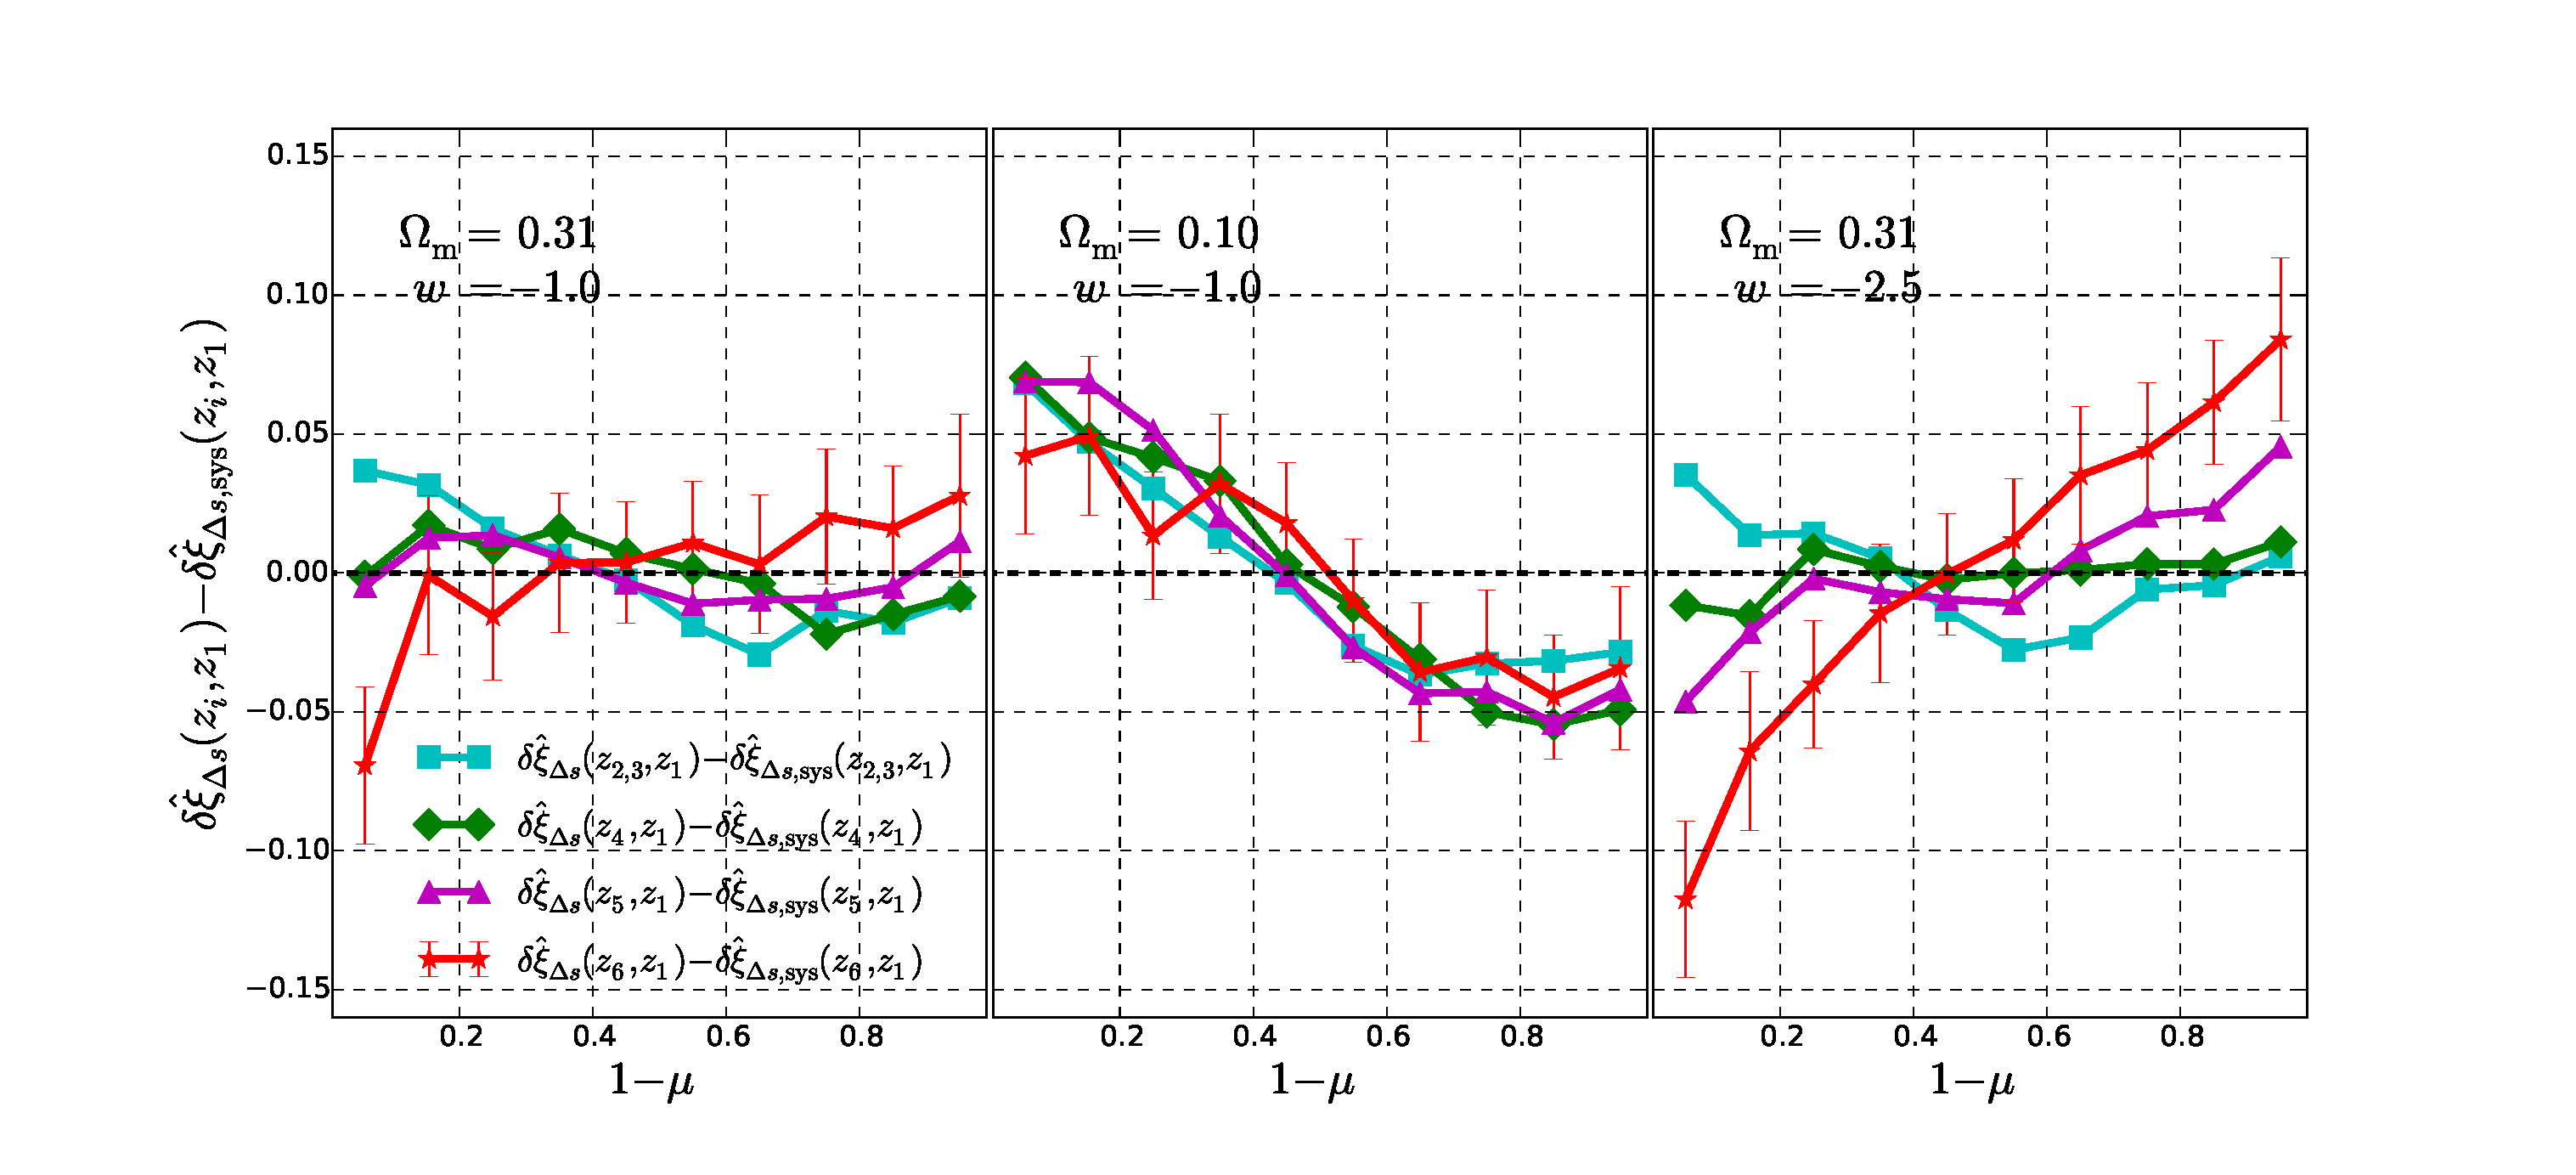
\includegraphics[width=18cm]{fig9_1.eps}
%   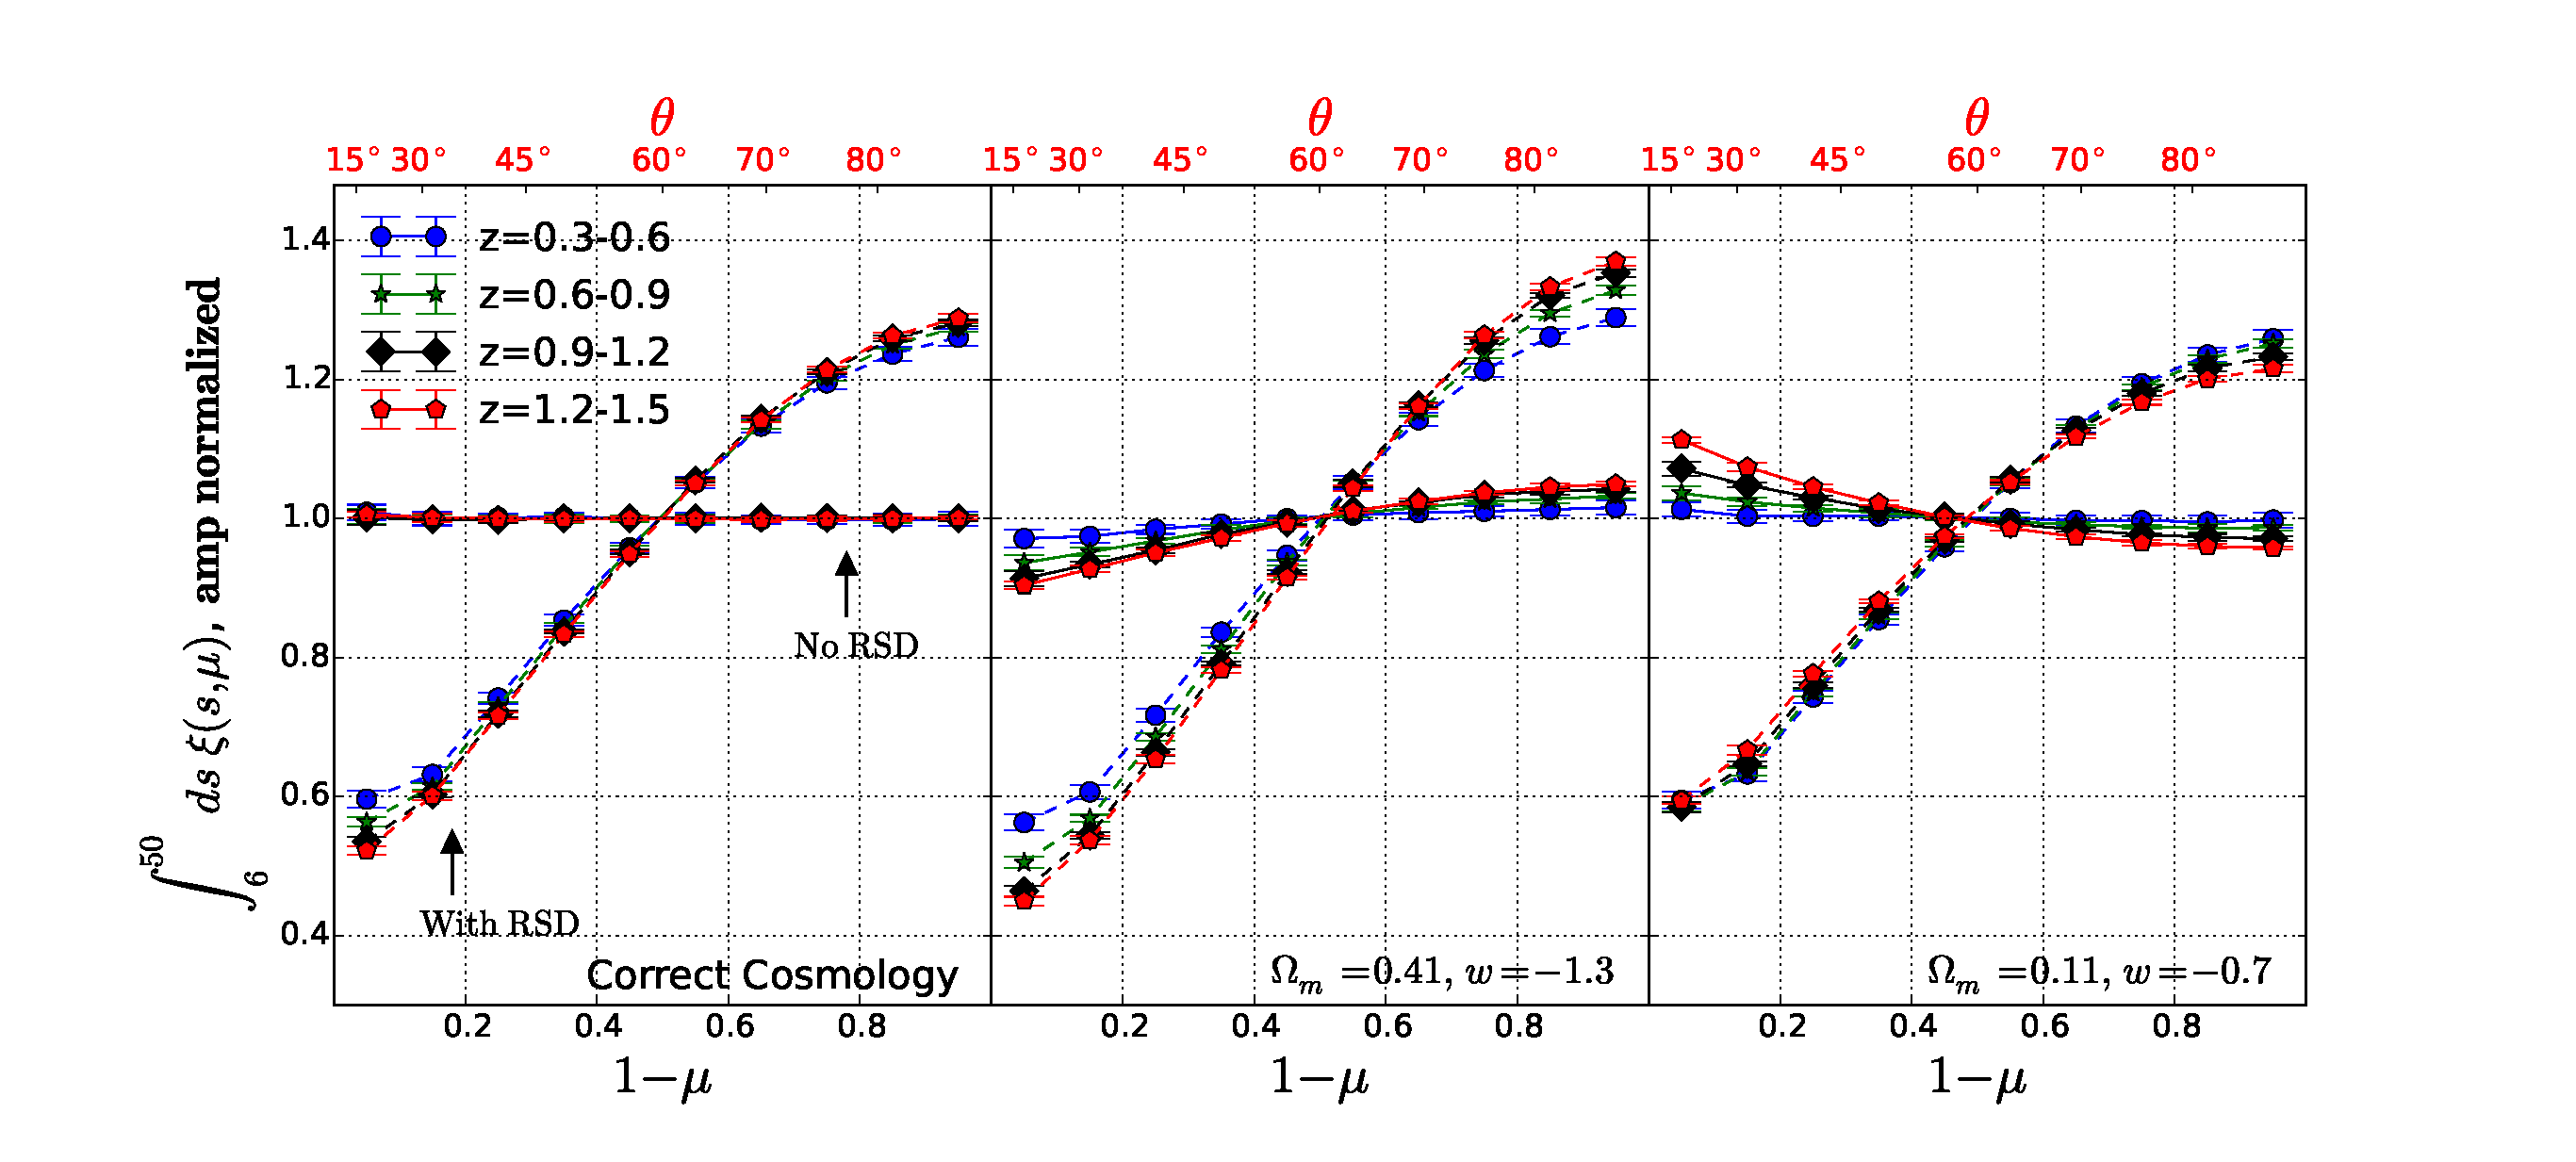
\includegraphics[height=8cm]{Tpcf--plot--Normed.eps}
%    \includegraphics[height=8cm]{smu.eps}
   }
   \caption{\label{fig_TpCF}
   Upper panels: $\hat \xi_{\Delta s}(\mu)$ measured for the BOSS DR12 galaxies,
   which are divided into six redshift bins.
   Measurements from the three bins in LOWZ are indicated in solid lines, 
   while those from CMASS are the dashed lines.
   We present the measurements in three cosmologies,
   the $\Omega_m=0.31$ $\Lambda$CDM (left), the $\Omega_m=0.1$ $\Lambda$CDM (middle),
   and a cosmology with $\Omega_m=0.31$, $w=-2.5$ (right).   
   %We adopt $s_{\rm min}=6$ $h^{-1}$Mpc and $s_{\rm max}=40$ $h^{-1}$Mpc for the integral over the scale of 2pCF.
   The angular dependence of 2pCF is measured in 10 bins within the range $0.01\leq1-\mu\leq1$.
   In the middle and right panels, the redshift dependence of AP distortions leads to clear redshift evolution of $\hat \xi_{\Delta s}(\mu)$.
   Lower panels: The redshift evolution of the $\hat\xi_{\Delta s}$ after systematics correction,  
   $\delta\hat \xi_{\Delta s}(z_i,z_1)-\delta\hat \xi_{\Delta s,\rm sys}(z_i,z_1)$
   (for details of their definitions, see Eq. (\ref{eq:deltahatxi}) and Sec. \ref{sec:syscor}).
   For clarity we combine the curves of $z_2$ and $z_3$, which fluctuate
   due to the relatively small sample sizes.
   The statistical significance is indicated by the 1$\sigma$ error bars of $\delta\hat \xi_{\Delta s}(z_6,z_1)-\delta\hat \xi_{\Delta s,\rm sys}(z_6,z_1)$.
   The curves are statistically consistent with 0 in the $\Omega_m=0.31$ $\Lambda$CDM cosmology,
    while they deviate from 0 at significant confidence levels in the $\Omega_m=0.1$ cosmology and the $w=-2.5$ cosmology.
   %showing the redshift dependence of AP effect.
   Applying the likelihood analysis described in Sec. \ref{sec:likelihood},
    the two latter models disfavored at 5.3$\sigma$ and 7.5$\sigma$ CL compared to the $\Omega_m=0.31$ $\Lambda$CDM cosmology.
   }
\end{figure*}

\section{Result}

We apply our method to the BOSS DR12 CMASS and LOWZ galaxies.
We present the results in this section.

\subsection{Redshift evolution in wrong cosmologies}\label{sec:redevolvxi}

%{\bf Figure: $\xi$ curves, in different cosmologies, without and with RSD}



The upper panels of Figure \ref{fig_TpCF} present the $\hat \xi_{\Delta s}$ measured for BOSS galaxies in three different cosmologies.
In the left panel we adopt the Planck cosmology, i.e., $\Lambda$CDM with $\Omega_m=0.31$;
%which should be {\it close to the truth}.
In the other two panels, we choose two sets of parameters ---
the $\Omega_m=0.1$ $\Lambda$CDM cosmology (middle) and the cosmology with $\Omega_m=0.31$ and $w=-2.5$ (right).
We split the BOSS DR12 galaxies into six redshift bins,
construct their 3D distribution in these three cosmologies
and then measure $\hat \xi_{\Delta s}(\mu)$ according to the procedure of the last section.

For a sample of galaxies with homogeneous, isotropic spatial distribution, 
the measured $\hat \xi_{\Delta s}(\mu)$ is statistically uniform.
The distortion in $\hat \xi_{\Delta s}(\mu)$ introduced by RSD is large.
There are two distinct features in this distortion.
At $0\lesssim 1-\mu \lesssim 0.1$, $\hat \xi_{\Delta s}(\mu)$ turns up as $\mu\rightarrow1$
due to the large FOG effect.
In other directions, the anisotropic clustering produced by the large scale flow creates a monotonic angle dependence of $\hat\xi_{\Delta s}(\mu)$. %a slope in the curve.
These patterns are evident in all cosmologies.


%\subsubsection{AP effect}


The additional angular dependence of $\hat \xi_{\Delta s}(\mu)$ introduced by AP is not as strong as RSD;
However, it is still visible. 
In the middle and right panels, % of Figure \ref{fig_TpCF},
%where there is clear redshift evolution of $\hat \xi_{\Delta s}$.
the choice of two incorrect cosmologies results in an enhancement of  $\hat \xi_{\Delta s}(\mu)$ due to the 
apparent stretch of non-linear structures in the LOS direction
%As a result, near LOS the value of $\hat \xi_{\Delta s}$ is enhanced 
\footnote{{\it Stretch of structure enhances the value of $\xi_{\Delta s}$}.
On relatively small scales, the strong clustering produces large values of $\xi$.
The apparent stretch of structure means the strong clustering on small scales are, apparently, shifted to larger scales:
at some fixed scale, we measured larger $\xi$ if there is apparent stretch.
The value of $\xi_{\Delta s}$, which is the integral of $\xi$ within fixed range of $s$, is also enhanced.}.
This effect is evident when we compare  $\hat \xi_{\Delta s}(\mu)$ in these two panels to that in the left panel.

More importantly, in incorrect cosmologies the redshift dependence of the AP effect results in a redshift evolution of $\hat \xi_{\Delta s}$.
This unique feature makes the AP effect detectable even with the existence of the large RSD effect. %distinguishable from the RDS distortion.
When $\Omega_m=0.1$ and $w=-1$ are adopted, 
the LOS stretch of structure becomes stronger at higher redshift (see Figure \ref{fig_xy});
as a result, the enhancement of $\hat \xi_{\Delta s}$ along the LOS 
becomes more significant at higher redshifts.
The opposite behavior is seen for the choice of $\Omega_m=0.31$ and $w=-2.5$.
%We see very evident redshift evolution of $\hat \xi_{\Delta s}$.
%I.e., the redshift dependence of AP effect results in redshift evolution of $\hat \xi_{\Delta s}$.
However, we do not see such obvious redshift evolution in the Planck cosmology, % is not so obvious.
 indicating that the cosmological parameters of the Planck cosmology are close to the correct ones.
%The Planck cosmology is widely accepted as to be close to the true cosmology parameters of our Universe and 
%There the AP effect is not strong enough to produce an evident redshift evolution.

The lower panels of Figure \ref{fig_TpCF} show the redshift evolution of $\hat\xi_{\Delta s}$ after systematics correction, 
i.e., the quantity $\delta\hat \xi_{\Delta s}-\delta\hat \xi_{\Delta s,\rm sys}$.
The result is statistically consistent to 0 in Planck cosmology -- 
In the four curves, almost all points are consistent with 0 at $\lesssim1\sigma$ confidence level (CL).
The only exception is the leftmost point of $\delta\hat \xi_{\Delta s}(z_6,z_1)-\delta\hat \xi_{\Delta s,\rm sys}(z_6,z_1)$,
 which is negative at $\sim$2 $\sigma$ CL.
This result could be due to the overestimation of $\delta\hat\xi_{\Delta s, \rm sys}(z_6,z_1)$ as discussed in Sec. \ref{sec:syscor}.
This behavior will not affect our derived cosmological constraints:
Dropping this measurement by imposing a cut $\mu<0.9$
  does not shift the constrained on $\Omega_m$-$w$ (the pink contour of Figure \ref{fig_contours}).

In the $\Omega_m=0.1$ cosmology and the $w=-2.5$ cosmologies, however,
the measured $\delta\hat \xi_{\Delta s}-\delta\hat \xi_{\Delta s,\rm sys}$ deviates 
from zero at significant confidence levels.
Applying the likelihood analysis described in Sec. \ref{sec:likelihood},
 they are disfavored at 5.3$\sigma$ and 7.5$\sigma$ CL compared to the Planck cosmology.
Since these two cosmologies deviates from the $\Omega_m=0.31$ $\Lambda$CDM cosmology with $\Delta \Omega_m = 0.21$ and $\Delta w = 1.5$,
roughly speaking, we expect our method able to constrain $\Omega_m$ and $w$ with 1$\sigma$ uncertainties of 0.04 and 0.2, respectively.


%Overall, the effect of RSD on the 2pCF is large but its redshift dependence is small.
%The correct cosmology corresponds to the case with the lowest change of $\hat \xi_{\Delta s}$ with $z$.
%Even with RSD, we can still correctly determine the true cosmology by using the relative change of $\hat \xi_{\Delta s}$ with redshift.


\subsection{Cosmological constraint}\label{sec:constraint}




We constrain $\Omega_m$ and $w$ through Bayesian analysis \citep{Bayesian},
which derives the probability distribution function (PDF) of some parameters $\bf \theta$ (=($\Omega_m,w$) in this paper)
given observational data $\bf D$, 
according to Bayes' theorem:
\begin{equation}
 P({\bf \theta}|{\bf D}) = \frac{P({\bf \theta})P({\bf D}|{\bf \theta})}{m({\bf D})}.
\end{equation}
Here $P(\bf \theta)$, the prior distribution of the parameters,
contains all the information about the parameters known from substantive knowledge 
and expert opinion {\it before} observing the data.
The marginal PDF of $\bf D$, 
$m({\bf D})=\int P({\bf D|\theta})P({\bf \theta})d{\bf \theta}$, 
is a normalization constant independent of $\theta$.
All the information about the parameter $\bf \theta$ that stems from the experiment
is contained in the function $P({\bf D}|{\bf \theta})$, 
the conditional PDF of the observation $\bf D$ given the value of parameter.

\begin{figure*}
   \centering{
   %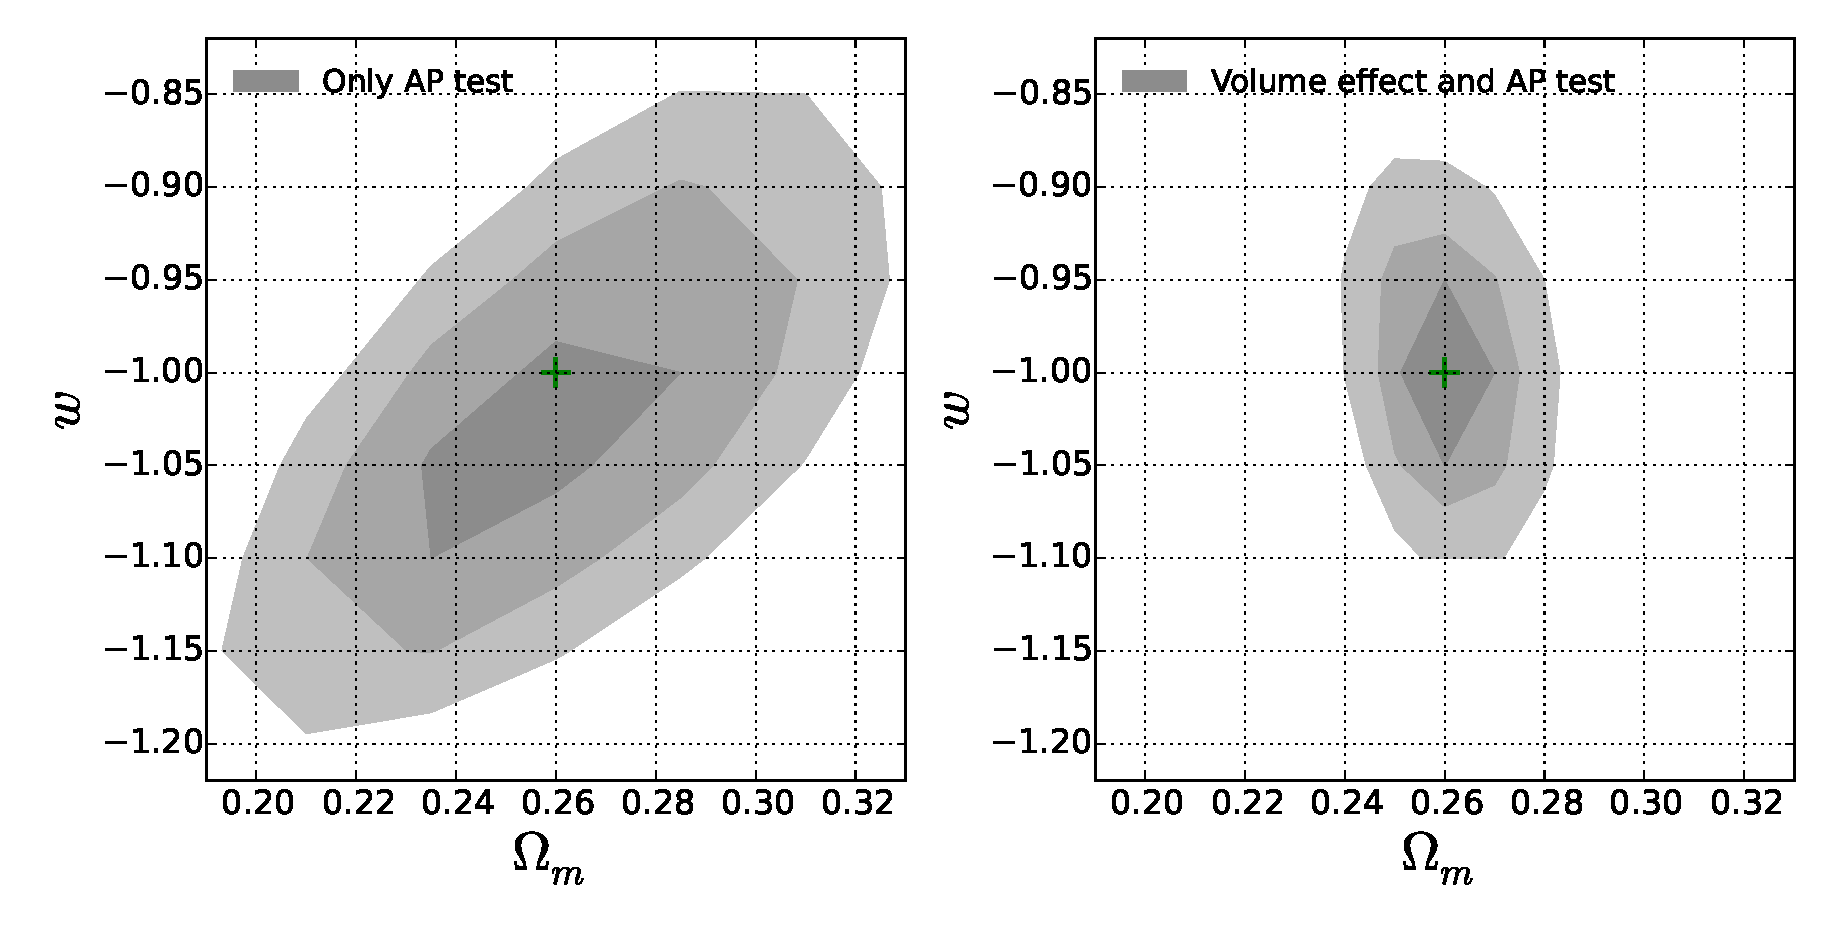
\includegraphics[width=7cm]{Tpcf--contour.eps}
   %\includegraphics[width=16cm]{Tpcf--contour-others.eps}
   %\includegraphics[width=16cm,natwidth=52,natheight=40]{fig10.eps}
   \includegraphics[width=16cm]{fig10.eps}
   }
   \caption{\label{fig_contours}
   Likelihood contours (68.3\%, 95.4\%) in the $\Omega_m-w$ plane from our method and other cosmological probes.
   %obtained from the BOSS DR12 CMASS and LOWZ samples.
   Using the BOSS DR12 galaxies within the redshift range $0.15< z< 0.693$, our method achieves tight cosmological constraints on $\Omega_m$ and $w$.
   The area of the 1$\sigma$ contour of our method is smaller than all other probes.
   Constraints from various probes are consistent with each other.
   See Sec. \ref{sec:constraint} for details.
   %in very good consistent with the other methods.
   }
\end{figure*}

In this analysis we simply assume flat priors for $\Omega_m$ and $w$,
and approximate $P({\bf D}|{\bf \theta})$ by a likelihood function $\mathcal{L}$
satisfying  $-2 \ln \mathcal{L}=\chi^2$;
the PDF of $\theta$ derived from our AP method takes the form
%The PDF cu is approximated by the {\it likelihood} function of $\mathcal{L}\propto \exp\left(-\frac{\chi^2}{2}\right)$.
%It is approximated by the {\it likelihood} function.
%So we have
\begin{equation}
 P({\bf \theta}|{\bf D}) \propto \mathcal{L} \propto \exp\left[-\frac{\chi^2}{2}\right].
\end{equation}
We use the {\texttt {COSMOMC}} software \citep{LB2002}
to obtain the Markov Chain Monte Carlo (MCMC) samples of $\theta$ following the PDF of $P({\bf \theta}|{\bf D})$.
Constraints on $\Omega_m$ and $w$ are derived from these samples.

The 68\% and 95\% likelihood contours of $\Omega_m$ and $w$ 
obtained from this analysis are shown in Figure \ref{fig_contours} (pink areas).
%For comparison, results from some other cosmological probes are also plotted.
Our AP method yields tight constraints on $\Omega_m$ and $w$ .
The mean values and 68\% CL are
\begin{equation}
 \Omega_m=0.314 \pm 0.038,\ \ w = -1.09 \pm 0.14.
\end{equation}
This result is consistent with the Planck $\Lambda$CDM cosmology within 1$\sigma$ \citep{Planck2015}.

We find the expected negative degeneracy between $\Omega_m$ and $w$.
At low redshift, increasing $\Omega_m$ and increasing $w$ have a similar effect on the cosmic expansion.
When one parameter is increased the other parameter can be decreased to counteract the AP effect
\footnote{At high redshift the direction of degeneracy completely changes. 
There the effect of $w$ is less important and the cosmic expansion is mainly governed by $\Omega_m$.
This behavior is why \cite{Li2015} obtained a positive degeneracy between $\Omega_m$ and $w$ from mock surveys 
spanning a wide range of $0< z < 1.5$.
The degeneracy direction between $\Omega_m$ and $w$ depends on the redshift range of the sample used in the analysis.
}.

For comparison, additional likelihood contours from other cosmological probes are displayed in Figure \ref{fig_contours}:
the JLA SNIa sample (green area, \cite{JLA}),
the BAO measurement from BOSS DR11 galaxies (bright yellow, \cite{Anderson2013}),
%\footnote{The CMASS and LOWZ samples from BOSS DR11 have a sky coverage of 8\,377 $\rm deg^2$ and a completeness of 97\%.
%They are very close to the DR12 samples.},
a combination of the BOSS DR11 BAO and the Hubble Space Telescope measurement of $H_0=70.6\pm3.3$ (dark yellow, \cite{Riess2011,E14H0}),
and the full-mission Planck observations of temperature and polarization anisotropies, released in 2015 (blue, \cite{Planck2015}).

%
The SNIa contours occupy a region similar to ours, but provide much weaker constraints. %has similar degeneracy to our method.% to us while the contour size is larger.
The direction of degeneracy is also similar.
%This is expectable.
By measuring the apparent magnitudes of type Ia supernovae distributed at different redshifts, 
 cosmologists can infer the luminosity distance $d_L$ as a function of redshift.
The JLA sample has similar redshift coverage to the BOSS DR12 galaxies,
which could be the reason for the similarity between the contours of the SNIa and our AP method.
%This is to some extent similar to our method, 
%which probes the redshift evolution of geometric distortion.
%which maybe the reason of the similarity 
%So the shapes and the positions of the contours from these two methods are a kind of close to each other.
%Comparing these two methods, we find our method has better constraining power.
%For SNIa probe, the degeneracy between $\Omega_m$ and $w$ is more serious and the contour extends to $\Omega_m=0$.

%The BOSS DR11 galaxies BAO measurements yields $D_V(z=0.32) = (1264 \pm 25 {\rm Mpc})(r_d /r_{d,\rm fid})$,
%$D_A(z=0.57) = (1421 \pm 20 {\rm Mpc})(r_d /r_{d,\rm fid})$, 
%and $H(z=0.57) = (96.8 \pm 3.4 {\rm km/s/Mpc})(r_{d,\rm fid} /r_d )$.
%Here $r_d$ is the drag epoch,
%$D_V(z)$ is the spherically averaged 2-point measurement of the BAO position, defined as $\left[cz(1+z)^2D_A(z)^2H^{-1}(z)\right]^{1/3}$, 
%and all measurements are presented as the ratio of the distance priors to their values in the fiducial cosmology \citep{Anderson2013}.
%At $z=0.57$, separating the clustering along and transverse to the LOS enables measurement of the sizes of the BAO ring in these two directions.


BAO itself can not effectively constrain $\Omega_m$ and $w$, 
since these parameters are highly degenerate with $H_0$ in determining the length scale.
Combining BAO with the $H_0$ measurements to break the degeneracy yields better constraint on the parameter space.
%The contour size is a bit larger than ours.
The direction of degeneracy of the combined constraint is roughly orthogonal to ours.
%This means we can combine these two LSS probes to break the degeneracy and significantly strengthen the constraining power.

CMB measurements provide a powerful probe of the geometry of the Universe,
but can not effectively constrain $\Omega_m$ and $w$ due to the strong degeneracy of the parameters.
%But combining CMB with the other probes can significantly shrink the volume of parameter space and tightens the constraint.
The CMB contour is almost orthogonal to the AP contour. 
%Contours from the two probes nicely overlapped with each other.
%In particular, our contour is well consistent with the Planck 2015 $\Lambad$CDM with $\Omega_m=0.308$.

Among all the individual cosmological probes, our method yields the most stringent 
constraint on $\Omega_m$ and $w$.
Our result is consistent with those of all other probes.
%Also, the degeneracy of our contour is different from most the other probes.
%We can take the advantage of this fact and tighten the constraint by combing them together.

Assuming that the five different cosmological probes of CMB, BAO, SNIa, $H_0$ and our method are 
statistically independent,
we combine the results by simply multiplying their likelihoods,
resulting in the total likelihood function
\begin{equation}\label{eq:likelihood}
\mathcal{L}_{\rm total} = \mathcal{L}_{\rm CMB} \times \mathcal{L}_{\rm BAO} \times \mathcal{L}_{\rm SNIa}\times \mathcal{L}_{\rm H_0}
 \times \mathcal{L}_{\rm Our\ AP}.
\end{equation}
The Planck team has released the {\texttt {COSMOMC}} outputs of MCMC samples
using CMB+BAO+JLA+$H_0$
\footnote{http://pla.esac.esa.int/pla/\#cosmology; 
Their BAO datasets include three sets of measurements from SDSS DR11 \citep{Anderson2013}, 6dFGS \citep{6dFGS} and SDSS MGS \citep{MGS}}.
We modify their MCMC samples (by changing the values of sample weight and likelihood)
 to include the likelihood of our method,
creating samples following the PDF of Eq. (\ref{eq:likelihood}).
The joint constraint from all five cosmological probes is
\begin{equation}
 \Omega_m = 0.304 \pm 0.007,\ w=-1.04 \pm 0.03.
\end{equation}
%{\bf which are the strongest constraints on these parameters obtained so far}
%{\bf AMTB: 
Our AP method plays an important role in strengthening the constraints on $\Omega_m$ and $w$.
As a comparison, combining CMB and our method yields $\Omega_m = 0.302 \pm 0.011,\ w=-1.05 \pm 0.04$,
while a combination of CMB and BAO yields $\Omega_m = 0.306 \pm 0.013,\ w=-1.03 \pm 0.06$.
%by combining the CMB and BAO measurements, %while .
In the absence of our method, a combination of SNIa, CMB, BAO and $H_0$
yields $\Omega_m = 0.306 \pm 0.009,\ w=-1.03 \pm 0.04$ \citep{Planck2015}.
% }

%\bibitem[Blake et al. (2011)]{WiggleZB}
%Blake, C., Kazin, E.A., Beutler, F., et al.
%2011, MNRAS, 418, 1707
%\bibitem[Kazin et al. (2014)]{WiggleZK}
%Kazin, E.A., Koda, J., Blake, C., et al.
%2014, MNRAS, 441, 352





\section{Concluding Remarks}

We apply the methodology developed in \cite{Li2014,Li2015} to BOSS DR12 galaxies.
In LSS surveys, the observed galaxy distribution appears anisotropic due to two reasons:
the contamination of galaxy redshifts due to the galaxy peculiar velocities, known as the RSD effect, 
and the error in the distance due to inaccurate cosmological parameters. %incorrectly assumed cosmological model for the coordinate transformation from redshift space to comoving space, known as the AP effect.
\cite{Li2014} reported that anisotropies produced by RSD effect are, although large,
close to uniform in magnitude over a large range of redshift,
while the degree of anisotropies introduced by AP varies with redshift. 
%We found that the redshift dependence of the anisotropy introduced by RSD is much less significant compared with the anisotropy caused by AP.
Thus we can use the redshift dependence of the anisotropic clustering of galaxies to constrain cosmological parameters without 
being much affected by RSD.

%The methodology developed in \cite{Li2015} was applied.
As in \cite{Li2015}, we investigate the redshift-dependence of clustering anisotropy by examining the 2pCF.
The 2pCF measured along different angular directions was characterized by the function $\hat \xi_{\Delta s}(\mu)$.
%In incorrectly adopted cosmological models, 
When the cosmological parameters governing the expansion history of the universe are incorrectly chosen,
the shape of this function evolves with redshift.
We split the DR12 galaxies into six redshift bins, measure the 2pCF in each redshift bin,
and search for the underlying true values of $\Omega_m$ and $w$ of our Universe % (assuming flat Universe)
by requiring minimal redshift evolution of $\hat \xi_{\Delta s}(\mu)$ across the six redshift bins.
We obtain tight constraints of $\Omega_m=0.314 \pm 0.038,\ \ w = -1.09 \pm 0.14$ from our method alone.

The constraints on $\Omega_m$ and $w$ from our AP method are tighter % in constraining the parameter space of $\Omega_m$ and $w$ 
than the other cosmological probes of SNIa, CMB, BAO, and $H_0$.
For the direction of degeneracy, %between $\Omega_m$ and $w$ in the constrained parameter space,
our method is similar to SNIa and orthogonal to CMB and BAO+$H_0$.
Combining the results of our method with those of other cosmological probes, 
we obtain tight constraints $ \Omega_m = 0.304 \pm 0.007,\ w=-1.04 \pm 0.03$.


\subsection{Comparison with other LSS probes}

Our method uses the anisotropic galaxy on scales from 6 to 40 $h^{-1}$Mpc.
%a novel analysis method extracting physical information encoded in LSS. % compared with the others.
%We look at the geometric distortion of LSS due to AP effect 
%clustering created by AP exhibits redshift evolution.
%Here the clustering scales we choose to look at in this analysis is 
Constrains on cosmological parameters are obtained from the redshift dependence of $D_A(z) H(z)$.

As a comparison, the BAO method uses the BAO feature in the 
clustering of galaxies on scales of 100-150 $h^{-1}$Mpc 
created by the oscillation of the baryon-photon plasma in the early Universe.
Measuring the BAO feature in 1D or 2D yields measurements of $D_V$ or $D_A$ and $H$ at some representative redshifts.
%So the principles and the physical information probed in these two methods are fundamentally different.

The AP methods proposed to date, such as those using 
galaxy pairs and voids, measure the rate of geometric distortion and are sensitive to $D_A(z) H(z)$,
while our method uses its the redshift dependence.
These methods can be combined together to fully utilize the physics of AP test.
Also, reducing the RSD effect 
through the redshift dependence could be 
applicable to these methods.

The topology method proposed by \cite{topology} 
uses the redshift evolution of the volume effect and is sensitive to the quantity $D_A(z)^2 / H(z)$.
Combing this method with ours can yield separate constraints on $D_A$ and $H$ 
for the same observational sample.
Constraints from the other statistical measures,
such as the distribution function of size or richness of LSS,
can be also combined \citep{Park2012,Park2015}.
%Analyzing the distortion of apparent galaxies clustering due to RSD,
%people can constrain the growth rate, the clustering strength and the galaxy bias.

Recently, \cite{MS2016} developed a novel method 
constraining cosmological parameters based on the high-level similarity of the emission measure in the cluster outskirts.
In incorrect cosmologies, the emission measure from clusters exhibits redshift dependence.
%This leads to tight constraints on the redshift evolution of the cosmic length scale.
Utilizing a sample of 320 galaxy clusters ($0.056<z<1.24$) observed with Chandra,
they achieve tight cosmological constraints comparable to ours.
The idea of this novel technique is to some extent similar to our method 
(seeking for the conservation of geometric quantity with redshift),
and could have promising future.
%and can be combined with our method to 

%The above LSS analysis methods, based on different concepts, 
%and probing different types of physical information, 
%are mutually complementary.
%It is worthy combining them together to comprehensively utilize the physical information encoded in the LSS 
%and derive tight constraints on parameters of cosmology. % and galaxy science.
%which is also fundamentally different from our method which is 


\subsection{Room for improvements}

This paper is the first application of this redshift dependent AP test to observed LSS data.
There remains considerable opportunity for improving the analysis methodology,
e.g., the optimized schemes of redshift binning and 
optimized choices of the scales of clustering (the values $s_{\rm min}$ and $s_{\rm max}$).
In this paper, the 2pCF is characterized by $\hat \xi_{\Delta s}(\mu)$.
It should be more advantageous to use 
the redshift evolution of 2pCF in two dimensions, i.e., $\hat \xi(s,\mu)$, 
to capture the full information.
It is also necessary to combine the 
information in the higher-order
statistic beyond the two point functions.
As pointed out in Sec. \ref{sec:caveats},
more theoretical and numerical studies on the 
redshift evolution of the RSD effect 
will remove the remaining small 
uncertainties in our results.

To avoid the difficulty of modeling galaxy bias we dropped the information of strength of clustering
through normalizing the amplitude of $\xi$.
In the case that we have good knowledge of galaxy bias, one can utilize the amplitude of $\xi$ to probe the redshift dependence of volume effect 
and obtain much tighter constraints.
\cite{Li2015} showed that
the area of constraining regions in $\Omega_m$ and $w$ space from the redshift dependence of the volume effect is 3.5 times smaller 
than that from the redshift dependence of the AP effect alone.

In this analysis, by reducing the RSD effect, 
%through looking at the redshift evolution,
we are able to use the galaxy clustering down to 6 $h^{-1}$Mpc.
This is a major advance in extracting the cosmological information 
on small scales where galaxy clustering is strong
and there are a lot of independent structures.

To make sure that the derived cosmological constraint is robust, 
in the procedure of systematics correction, 
one should construct many mock surveys in which the RSD and other systematic effects are reliably modeled.
%It could be crucial to adopt a good galaxy assignment scheme, 
%such as the MBP-galaxy correspondence model developed in \citep{hong2016}.
%adopted in this analysis, could be crucial.
%So we can obtain an accurate estimation of systematic effect.

It would also be helpful to investigate the effect of galaxy properties.
For example, in case of a dense survey containing galaxies with various properties, 
one can split the galaxy sample into subsamples with different galaxy properties, 
derive cosmological constraints from these subsamples, 
and check the consistency of the results. 

%Our method is to some extent very similar with the methods using the overall shape of 
%the power spectrum or correlation function Park \& Kim (2010) Shoji et al. 2009 {\bf AMTB: Read them and check }.
%But we have one addition that uses the shape in a set of redshift slices to reduce the RSD effect.

%This is one of the reasons why our method is powerful.
%for the strong power of our method -- the small scale galaxy clustering contains abundant information.
%In future the development of simulation technique may enable us to accurately modeling galaxy clusterings on even smaller scales 
%and makes our method more powerful.

\subsection{Synergies with future observations}

The constraining power of our method is proportional not only to the size, 
but also to the redshift coverage of the galaxy sample.
In this analysis we utilize 1\,133\,326 BOSS DR12 galaxies covering $0.15< z < 0.693$.
Future redshift surveys such as eBOSS \citep{eBOSS}, EUCLID \citep{EUCLID}, and DESI \citep{DESI}
will have larger sample sizes and wider redshift coverage.
Our method is expected to yield much tighter cosmological constraints
and can be applied to constrain wider classes of 
cosmological models when these data are available.
%In the future we will have LSS surveys of 
% having much wider redshift coverage and much larger number of observed galaxies.
%{\bf Introducing the redshift range and galaxy numbers of future surveys?: eBOSS, DESI, LSST, ...?}
%Being able to utilizing small scale clustering information a denser survey will be also helpful to improve the power of our method.
%Even for the regions already probed by the current SDSS-III survey, 
%there is still large potential to improve the power of constraint by conducting a deeper survey to increase the S/N.

In this analysis we assume a flat Universe to constrain $\Omega_m$ and $w$.
Our method should be sensitive to all other cosmological parameters governing the cosmic expansion history,
e.g., the curvature of the Universe, 
and the other dark energy parameters.

Overall, the future of our method is extremely promising. 
With the progressive development of LSS experiments, 
we expect it to play an important role in deriving cosmological constraints from LSS surveys.
%and yielding fruitful out-comings.



\section*{Acknowledgments}

We thank the Korea Institute for Advanced Study for providing computing resources (KIAS Center for Advanced Computation Linux Cluster System).
%We thank Seokcheon Lee and Graziano Rossi for many helpful discussions.
We would like to thank Ho Seong Hwang, Francisco-Shu Kitaura, Benjamin L'Huillier, Donghui Jeong, Teppei Okumura, Will Percival, Hyunmi Song 
and Yi Zheng for kind helps and helpful discussions.
This work was partially supported by the
Supercomputing Center/Korea Institute of Science and
Technology Information with supercomputing resources
including technical support (KSC-2013-G2-003).

Based on observations obtained with Planck (http://www.esa.int/Planck), 
an ESA science mission with instruments and contributions directly funded by 
ESA Member States, NASA, and Canada.

Funding for SDSS-III has been provided by the Alfred P. Sloan Foundation, the Participating Institutions, the
National Science Foundation, and the U.S. Department of Energy Office of Science. 
The SDSS-III web site is http://www.sdss3.org/. 
SDSS-III is managed by the Astrophysical Research Consortium for the Participating Institutions
of the SDSS-III Collaboration including the University of Arizona, the Brazilian Participation Group, Brookhaven
National Laboratory, Carnegie Mellon University, University of Florida, the French Participation Group, 
the German Participation Group, Harvard University, the Instituto de Astrofisica de Canarias, the Michigan State/Notre
Dame/JINA Participation Group, Johns Hopkins University, Lawrence Berkeley National Laboratory, Max Planck
Institute for Astrophysics, Max Planck Institute for Extraterrestrial Physics, New Mexico State University, New
York University, Ohio State University, Pennsylvania State
University, University of Portsmouth, Princeton University,
the Spanish Participation Group, University of Tokyo, University of Utah, Vanderbilt University, University of Virginia, 
University of Washington, and Yale University.


\appendix

\section{A. Robustness Tests}\label{sec:RBtest}

We conduct a series of tests to check the robustness of our results.

The cosmological constraints presented in Sec. \ref{sec:constraint} (hereafter the ``main results'') are derived using 
the following options (hereafter the ``default options''):
\begin{itemize}
 \item We adopt $s_{\rm min}=6 h^{-1} {\rm Mpc},\ s_{\rm max}=40 h^{-1} {\rm Mpc}$ in the integrated 2pCF
 ($\xi_{\Delta s} (\mu) \equiv \int_{s_{\rm min}}^{s_{\rm max}} \xi (s,\mu)\ ds$).
 \item The effects of systematics are estimated from the HR4 mock galaxies. 
 When constructing the mocks, to determine when a satellite galaxy is disrupted,
 we adopt the J08 model to calculate the satellite galaxy merger timescale.
 \item In total 72 sets of HR3 PSB mock surveys are used to construct the covariance matrix.
 \item We drop the angular region $1 - \mu < 0.01$, to mitigate the effects of fiber collisions and redshift failures.
\end{itemize}


\begin{figure*}
   \centering{
   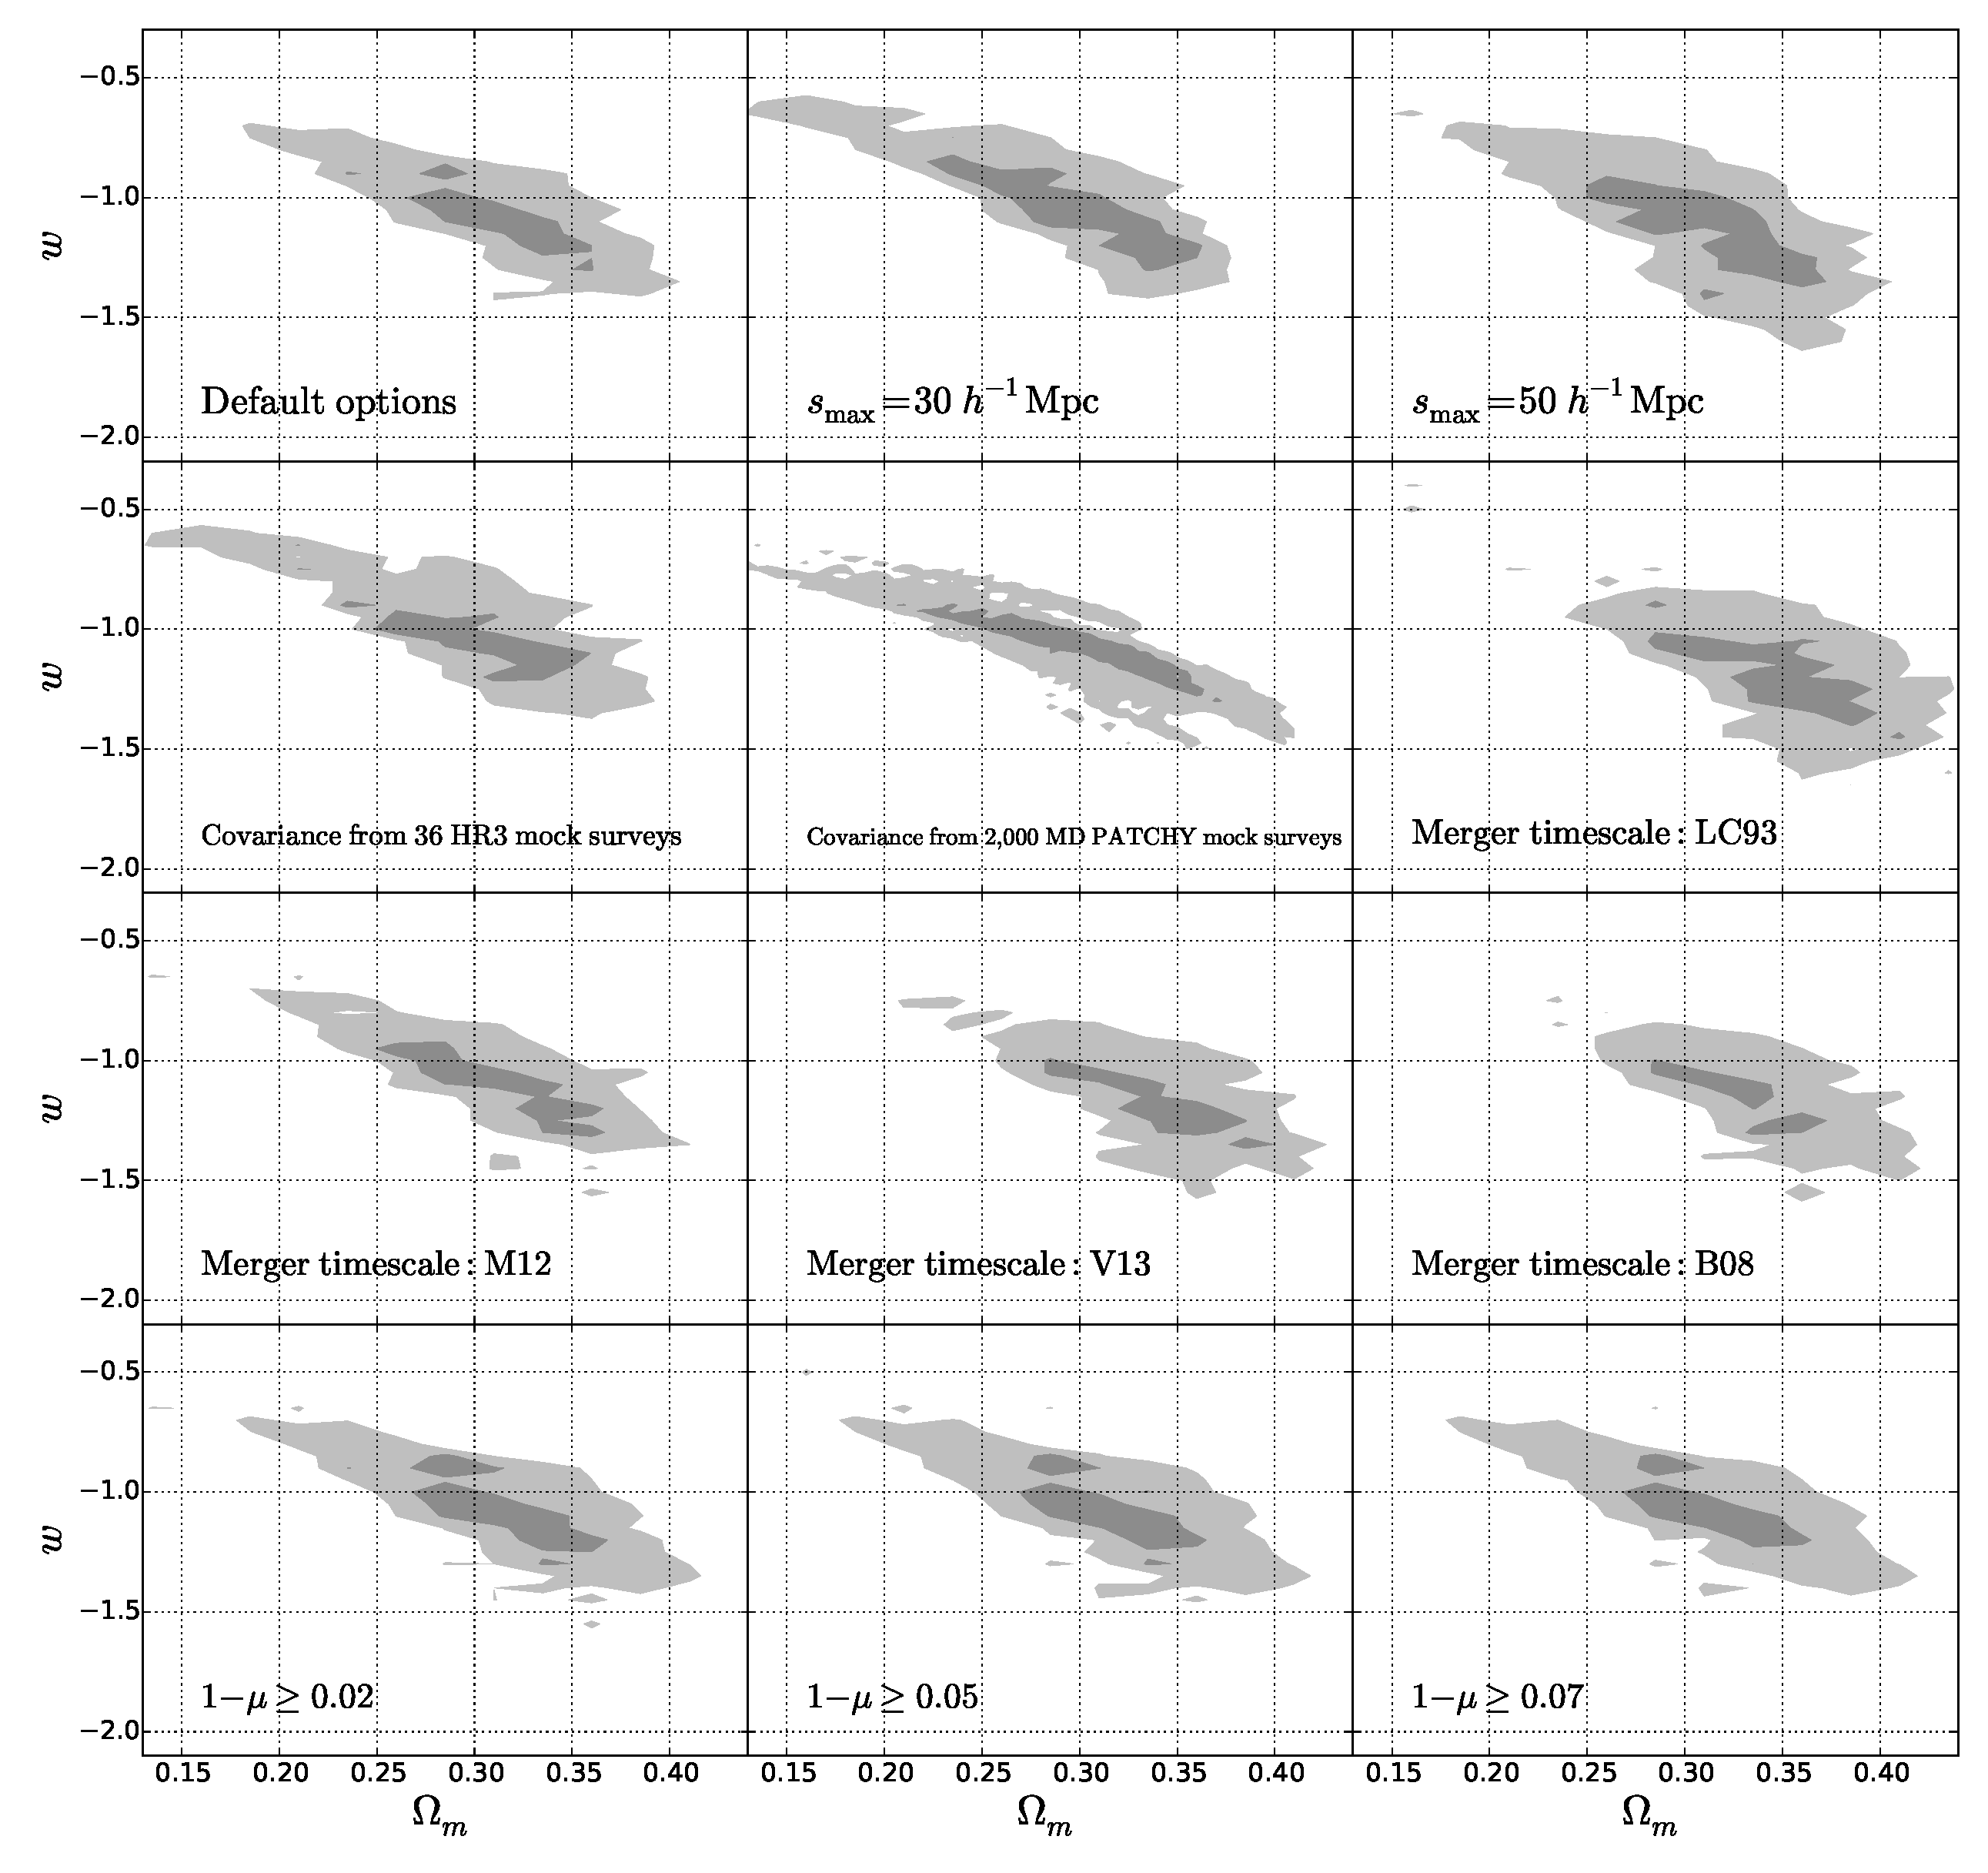
\includegraphics[width=14cm]{fig11.eps}}
   %\includegraphics[width=5.9cm]{Tpcf--contour-nummock-36.eps}}
   \caption{ \label{fig_contour_RB}  
   Likelihood contours (68\%, 95.4\%) in the $\Omega_m$-$w$ plane, derived by applying our AP method to the BOSS DR12 galaxies.
   The upper-left panel displays the main results derived using the default options.
   %i.e. using $s_{\rm min}=6h^{-1}{\rm Mpc}$, $s_{\rm max}=40h^{-1}{\rm Mpc}$, $1 - \mu \ge 0.01$,
   %72 sets of HR3 PSB mocks for covariance estimation,
   %and J08 model to compute the merger timescale model in the construction of mock surveys.
   The other panels show the contours when the options are altered one by one.
   %We find good consistency among these contours. 
   }
\end{figure*}

We check whether the results are sensitive to these options.
We modify the above options one by one, 
derive the corresponding cosmological constraints, 
and check how much they deviate from the main results.
%and are compared with the constraints derived using the default option set.
We present this information in Figure \ref{fig_contour_RB}. %displays the many sets of cosmological constraints derived with various sets of modified options.
%The upper-left panel shows the result using the default options, 
%while the other many panels display the result after changing one of these options.

To be efficient, we adopt a coarser grid with $\delta \Omega_m=0.025,\ \delta w=0.05$ when covering the parameter space.
%Although the obtained contours look a little coarse, 
This resolution is high enough for the purpose of testing our methodology.


\subsection{$Different\ s_{\rm max}$}

The upper-panel of Figure \ref{fig_contour_RB} shows the main results, 
the cosmological constraint when the default options are adopted. %There we use $s_{\rm max}=40 h^{-1}{\rm Mpc}$. 
The results for $s_{\rm max}=30,\ 50 h^{-1}{\rm Mpc}$ are displayed in the middle and right panels of the first row.
%While the default choice of $s_{\rm max}=$ 40 $h^{-1}$Mpc gives the tightest constraint, 
The three choices of $s_{\rm max}$ results more or less similar to the main results.

\subsection{$Number\ of\ mocks\ for\ covariance\ estimation$}

In this analysis we use a set of 72 mock surveys sampled from HR3 to compute the covariance matrix.
We check whether the relative small number of mock surveys could produce significant bias in the derived cosmological constraint.

We take half of the mock surveys to compute the covariance matrix;
the result is presented in the second row of Figure \ref{fig_contour_RB}.
Our main result from 72 mocks gives slightly tighter constraint and less noisy contours than the results from 36 mocks.
The locations of contour center are similar, and statistically are quite close to each other.

Using 36 mocks we must adopt $n_\mu\lesssim20$ for the binning of $\xi_{\Delta s}(\mu)$,
so it is expected that the results are slightly weaker than the results of using 72 mocks (where we take $n_{\mu}\leq40$).

We further take the 2,000 sets of MultiDark PATCHY mock catalogues \citep{MDPATCHY} to compute the covaraince matrix.
%This set of mock surveys have been adopted for the error estimations of the 2pCF and power spectrum measurement of the BOSS galaxies \citep{Alam2016}.
Following Hartlap et al. (2006) and Percival et al. (2014), we correct the covariance matrix
for the statistical bias and scattering.
The obtained results are consistent with the main results.
The constrained area has a small extension in the upper-left corner, which will not affect the combined cosmological constraint.

%The constraints while using 36 mocks for covariance matrix appears a little weaker.
%The reason is that, the smaller number of mocks, the smaller number of binning allowed in the analysis. 
%As discussed in Sec. \ref{sec:binningscheme}, in our main analysis we are able to use as much as 40 bins in the region $0.01\leq\mu\leq1$.
%When using 36 mocks we limit the largest bin number to 20, which leads to slightly weaker constraint.


\subsection{$Mock\ galaxies\ for\ systematic\ correction$}

In the construction of HR4 mock galaxies \citep{hong2016}, 
the J08 model \citep{jiang2008}, a model derived from cosmological simulations, 
was adopted as the default option to calculate the merger timescale and to determine when a satellite galaxy is completely disrupted.

\cite{hong2016} also considered four alternative models for the calculation of merger timescale:
1) the LC93 model \citep{LC93} based on analytic calculation, 
2) the B08 \citep{B08} and 3) the V13 \citep{V13} models based on isolated simulations,
and 4) the M12 model \citep{M12} based on cosmological simulation.
%Among the five merger timescale models, 
%J08 was found to result in mock galaxies with properties and 2pCF best matching the observational data.
Among the five merger timescale models, 
J08 model produces mock galaxies having properties and 2pCF best agree with the observational data \citep{hong2016};
%So it was adopted in our main analysis.with
the LC93 model, having the shortest merger timescale among the five models,
produces galaxies with properties and 2pCF most deviated from the observations.


\begin{figure*}
   \centering{
   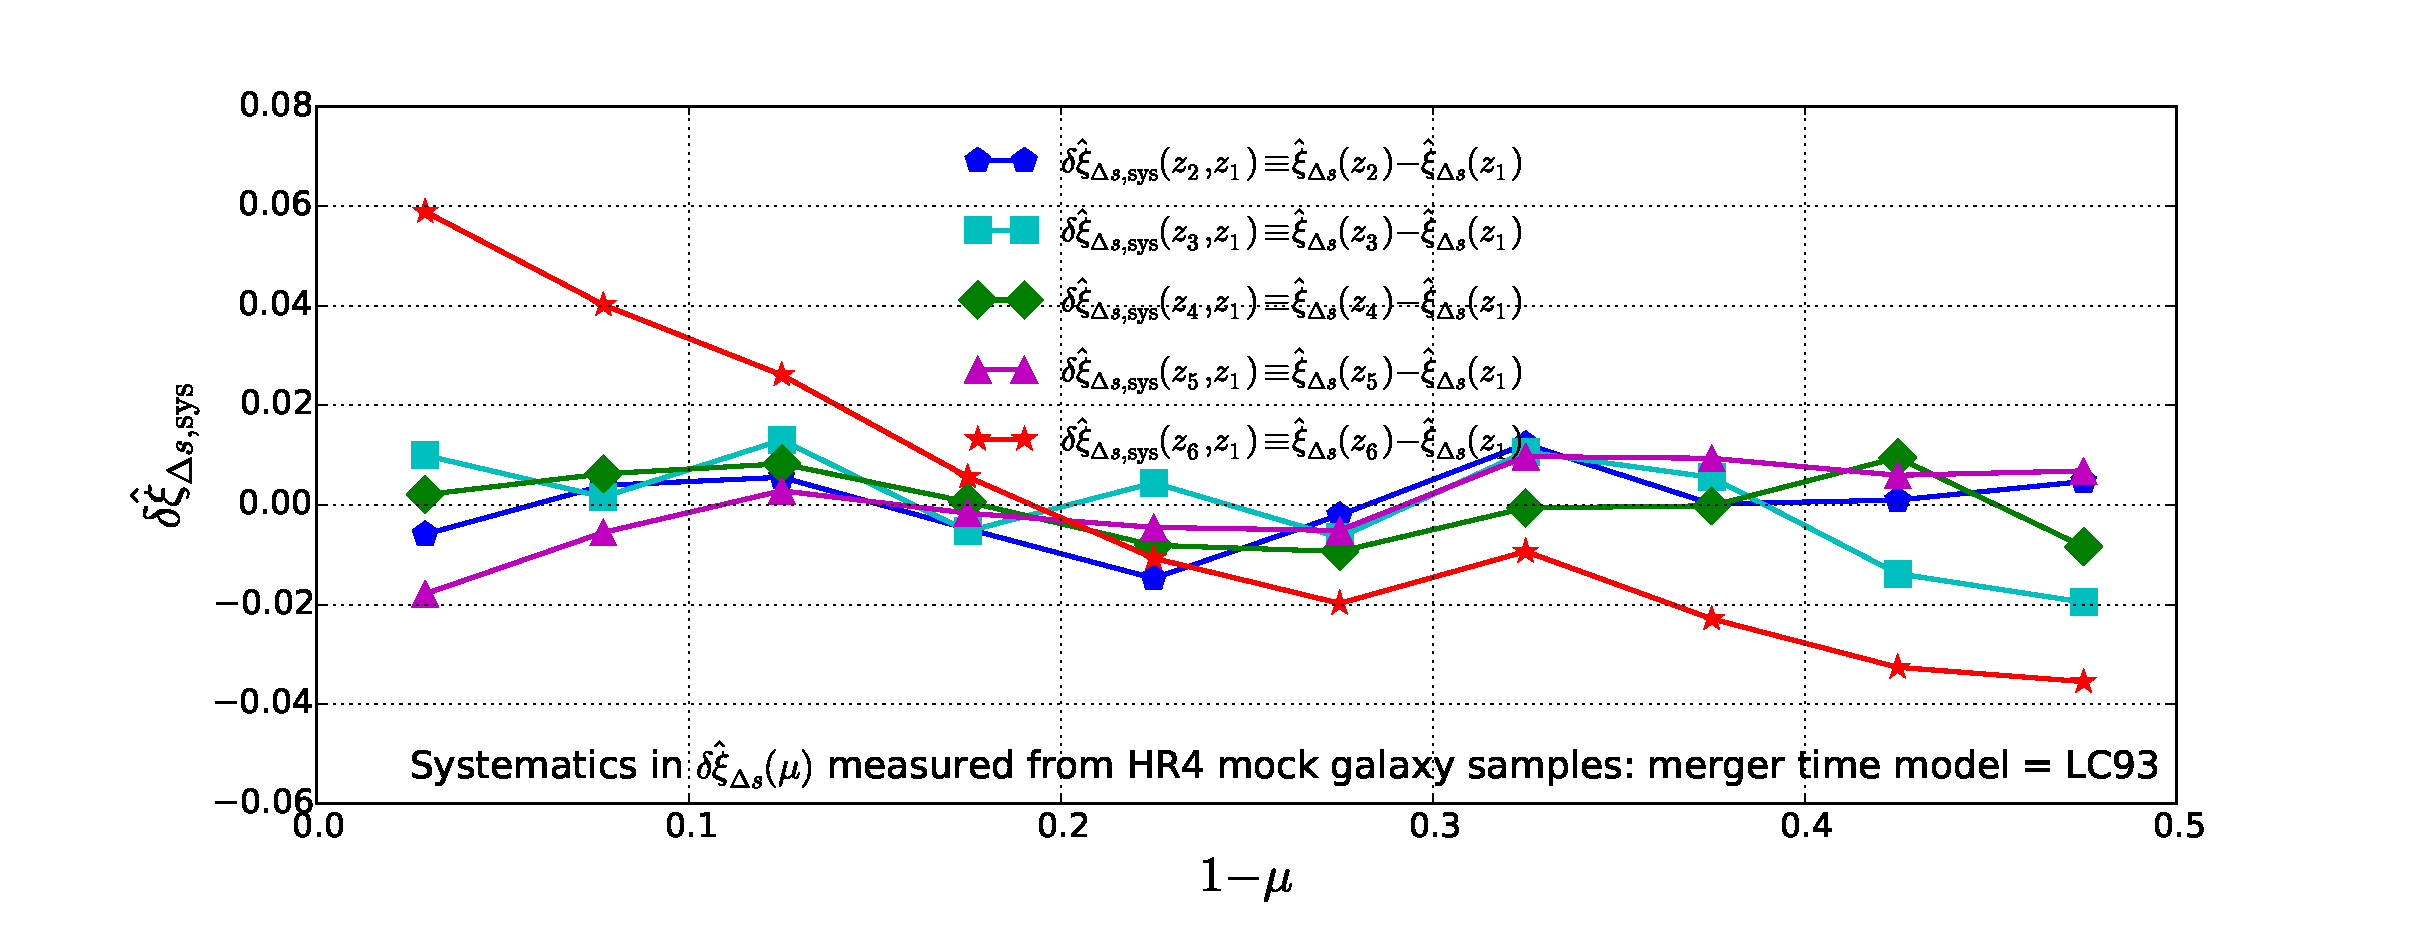
\includegraphics[width=16cm]{fig12.eps}
   %\includegraphics[height=9cm]{Tpcf-sys.eps}
   }
   \caption{\label{fig_sys_LC93}
   %Apparent distortion of objects in four wrongly assumed cosmologies, assuming a true cosmology of .
   Systematics in $\delta \hat \xi_{\Delta s}$, measured from the HR4 mock galaxies
   with the LC93 model adopted as the merger timescale model.
   Compared with the main result using the merger timescale model J08 (Figure \ref{fig_sys}), 
   there is a $\sim 25\%$ change in the amplitude of $\delta \hat \xi_{\Delta s}$.
   % so the measured $\hat\xi_{\Delta s}(\mu)$ has larger (smaller) values at $\mu\rightarrow1$ ($\mu\rightarrow0$) 
   % compared with the others.
   %See Sec. \ref{sec:syscor} for details.
   %The values are estimated from the HR4 mock galaxies. % and subtract its contribution.
   }
\end{figure*}

%To check whether our result is sensitive to these merger timescale models,
We adopt mock surveys created using the four alternative models to
measure the systematic correction $\delta \hat\xi_{\Delta s, {\rm sys}}$
and derive the cosmological constraints.
The difference between the $\delta \hat\xi_{\Delta s, {\rm sys}}$ estimated from the J08 model and the other models is $5\%-25\%$.
As an example, Figure \ref{fig_sys_LC93} presents the systematics correction estimated using LC93,
which has a $\sim25\%$ difference from the J08 estimation.

Nevertheless, Figure \ref{fig_contour_RB} shows that, 
when the alternative models adopted, 
the cosmological constraints are consistent with our main results;
the discrepancy is $\lesssim0.3\sigma$.

%In case of using the $z=0$ snapshot data rather than the lightcone galaxies to construct mock surveys,
%we find the contour slightly shifted to the upper-left direction.
%Statistically, 

%Also, the shifts of contours mainly happens along the upper-left to lower-right diagonal.
%This means the joint constraint result, the constraint when combined with the other cosmological probes such as CMB, will not be very affected,
%since the CMB contour basically lies in the lower-left to upper-right diagonal.


\subsection{$Cut\ on\ \mu$}

%We checked whether the result is sensitive to the range of angular bins.
In our default options, we take $1 - \mu\ge0.01$.
For comparison, Figure \ref{fig_contour_RB} presents the cosmological constraints using the limits 
%0.02, 0.05, 0.07 and 0.1.
0.02, 0.05 and 0.07. 
A larger limit means we abandon more angular regions near the LOS.
%That will make the result less affected by the factors such as fiber collision.
We find that changing the cut has little effect on the cosmological constraints.
%Even for the case of $1 - \mu\ge0.1$,
%where 10\% of the angular region is dropped,
%the constraints are still fully consistent with the main results.
%This suggests that our main result is less affected by the fiber collision.

This test suggests that our result is not affected by the fiber collisions and redshift failures.
%In the observational data, these effects are taken into consideration by reweighting the nearest neighbor of the galaxy.
%Also, we add the fiber collision effect when constructing mock surveys.
If fiber collisions and redshift failures have any sizable effect,
since they mainly affect the angular region close to LOS,
one expects a systematic variation of the cosmological constraints when varying the limit on $1-\mu$.
%Such a variation was not detected in this test.
%so the fiber collision and redshift failure effects are certainly removed 



\subsection{$Different\ s_{\rm min}$}

%\subsection{A2. Different $s_{\rm min}$}

Among the different options, %affecting our cosmological constraint, 
the one most likely to affect our results is $s_{\rm min}$.
%the smallest scale that are taken into account in the analysis.
%This is expectable. 
The 2pCF has relatively large values on smaller scales
%On small scales, the value of 2pCF is relatively large
(e.g. for the CMASS galaxies $\xi\approx10,5,1,0.25,0.05$ at $s=2,4,10,20,40 h^{-1}{\rm Mpc}$).
Varying $s_{\rm min}$ can dramatically change the value of $\xi_{\Delta s}(\mu)$,
and thus is likely to have large effect on the result.

A series of input-output tests are conducted to check whether the derived constraints depend on $s_{\rm min}$.
The linear regression of the $\delta\hat\xi_{\Delta s}$ (of the observational sample) 
measured in the WMAP5 cosmology ($\Omega_m=0.26$ $\Lambda$CDM) 
is adopted as $\delta\xi_{\Delta s, \rm sys}$. 
We then follow the procedures of Sec. \ref{sec:methodology} to derive cosmological constraint.
%In that case we expect the WMAP5 cosmology being the best-fit.

\begin{figure*}
   \centering{
   %\includegraphics[width=12cm]{Tpcf--contour-diffsmin-dashcontours.eps}}
   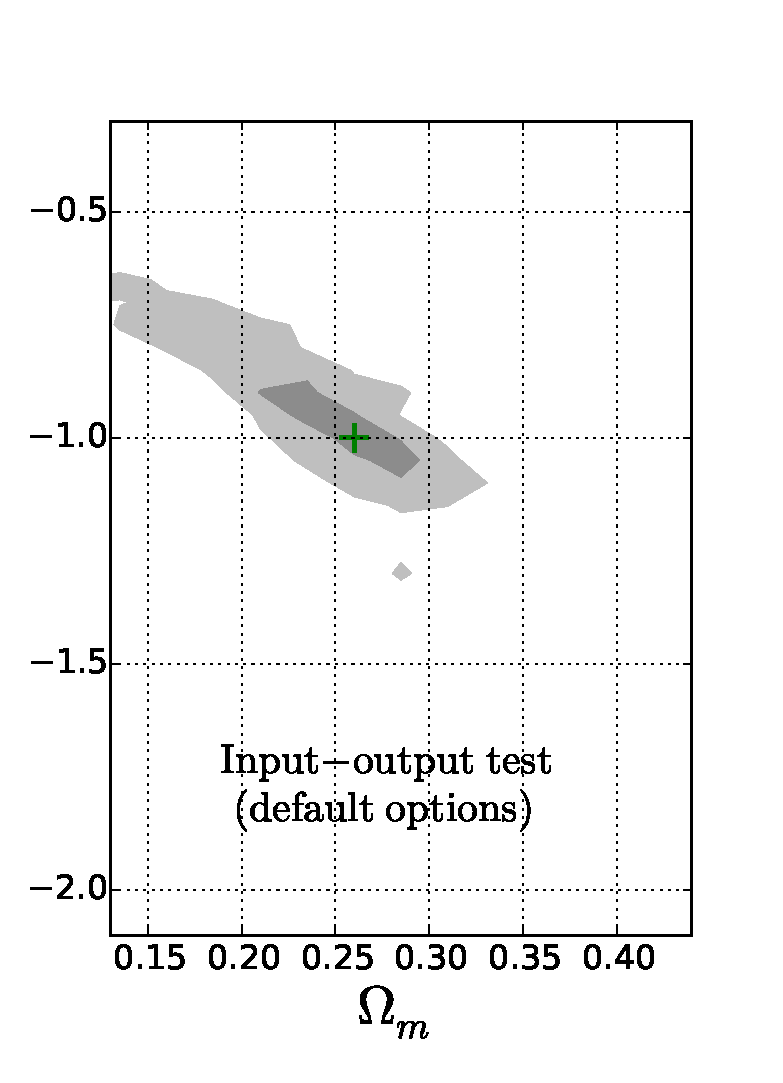
\includegraphics[width=5.7cm]{fig13_0.eps}
   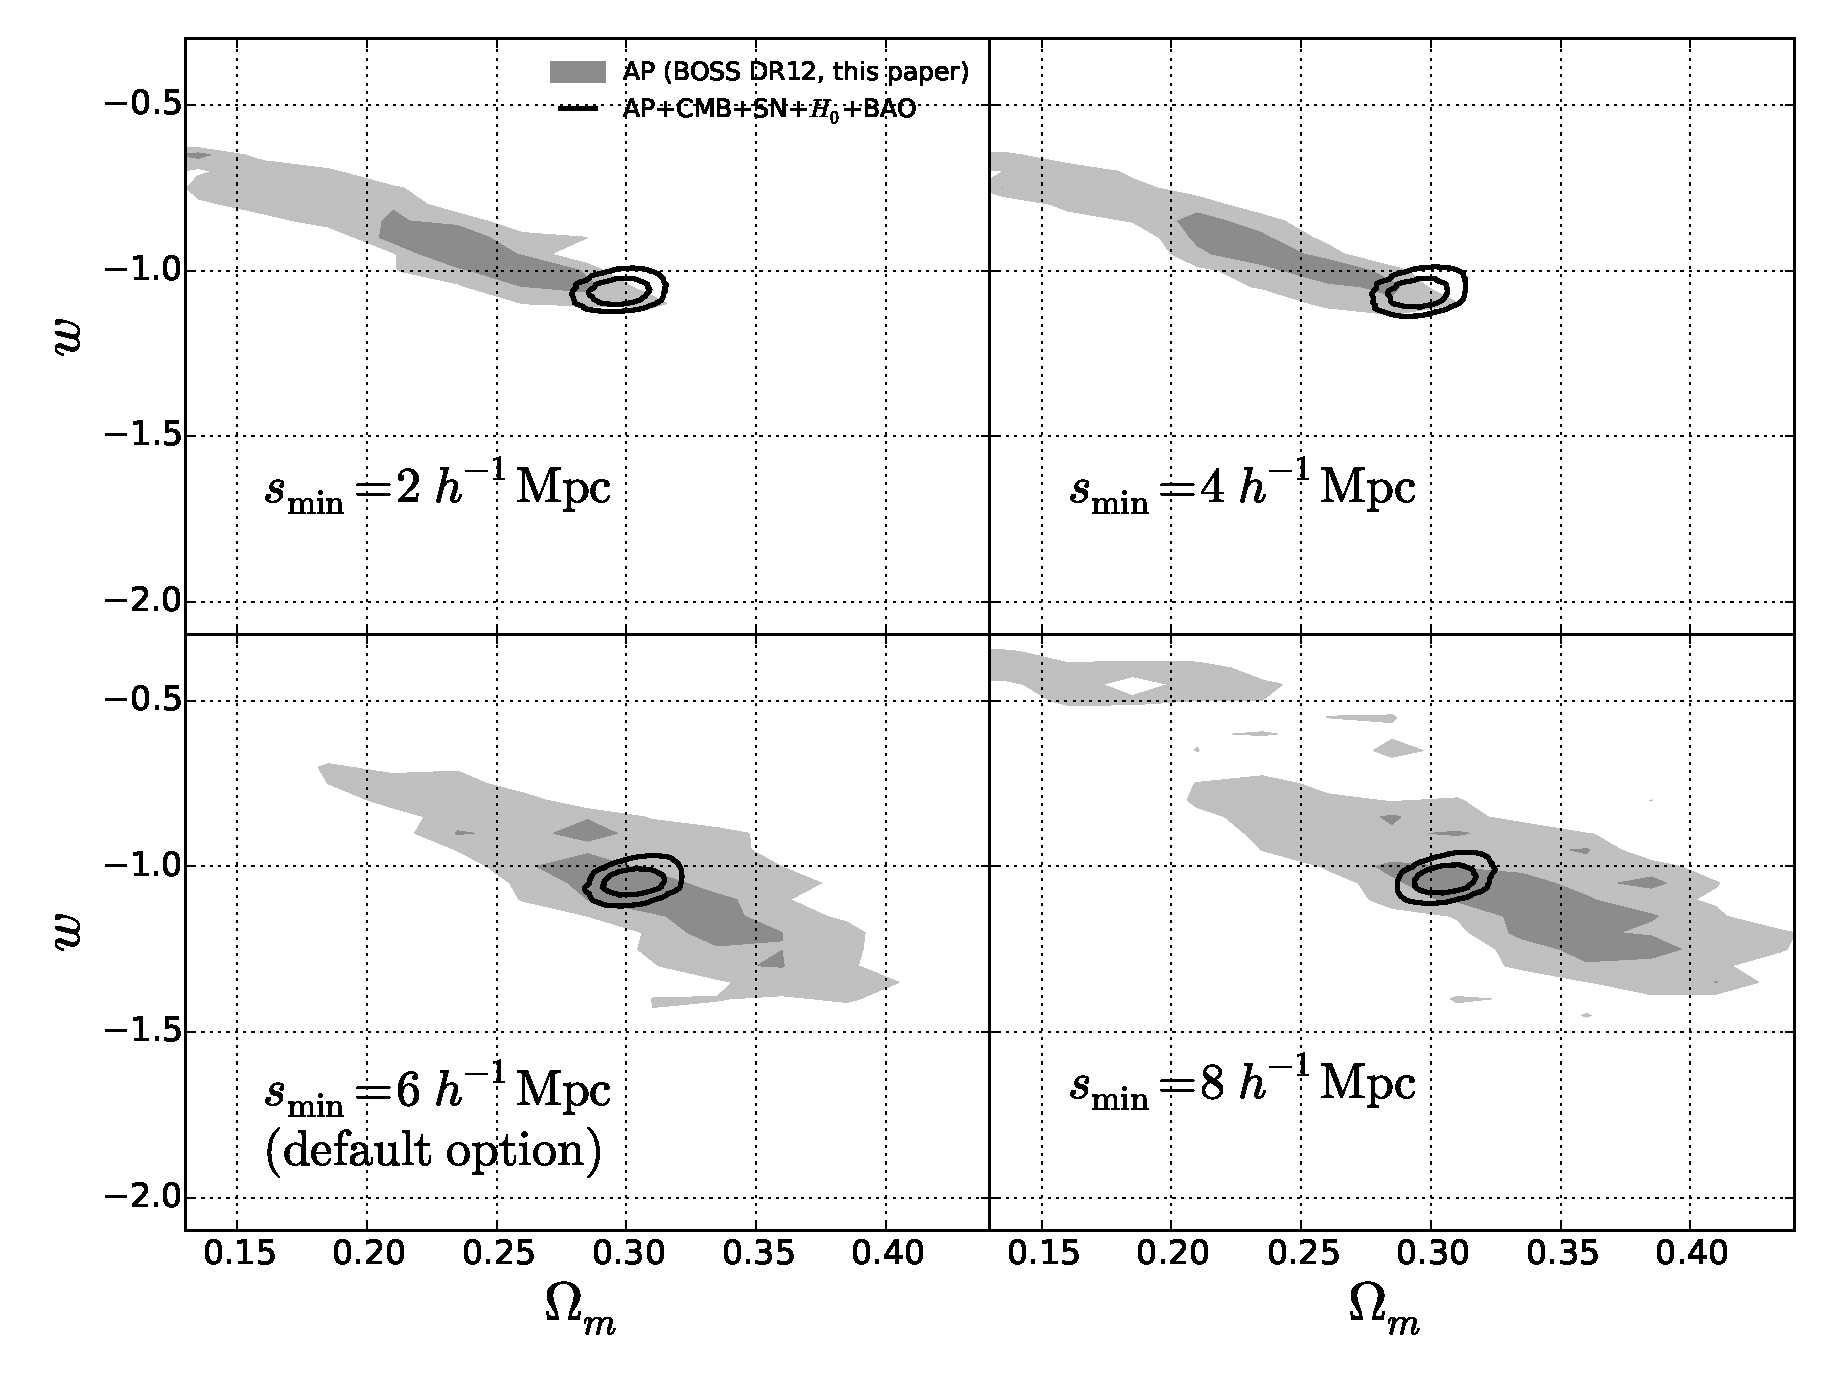
\includegraphics[width=10cm]{fig13_1.eps}}
   %\includegraphics[width=5.9cm]{Tpcf--contour-nummock-36.eps}}
   \caption{ \label{fig_contour_diffsmin} 
   Left panel: The input-output test in case of using our default options.
   The derived cosmological constraints are fully consistent with the input WMAP5 cosmology (marked by green plus).
   Right panels: Likelihood contours (68\%, 95.4\%) in the $\Omega_m$-$w$ plane for using $s_{\rm min}=2,4,6,8\ h^{-1} {\rm Mpc}$.
   Gray filled contours are cosmological constraints derived using our AP analysis.
%    From the input-output test we find $s_{\rm min}$
   %For $s_{\rm min}=2,4,8\ h^{-1}{\rm Mpc}$, some correction of the likelihood map was made based on the result of their input-output tests.
   %After the correction they are close to the result using the default option $s_{\rm min}=6h^{-1}\rm Mpc$.
   For $s_{\rm min}=2,4h^{-1}{\rm Mpc}$, the contours are shifted to the upper-left corner, 
   but the deviation from the $s_{\rm min}=6h^{-1}{\rm Mpc}$ is $\lesssim1\sigma$.
   The black solid contour lines show the constraint when combined with CMB+BAO+JLA+$H_0$.
   %The dashed contour lines show the combined constraints in case of no correction made for $s_{\rm min}=2,4,8\ h^{-1}{\rm Mpc}$. 
   The combined result is rather insensitive to choices of $s_{\rm min}$.}
\end{figure*}

When adopting $s_{\rm min}=6\ h^{-1}{\rm Mpc}$, the best-fit cosmology is exactly what we expect: the WMAP5 cosmology, 
i.e. the input cosmology is successfully recovered (left panel of Figure \ref{fig_contour_diffsmin}).
So $s_{\rm min}=6\ h^{-1}{\rm Mpc}$ is adopted as the default option in our analysis.
%When adopting different a $s_{\rm min}$ of $2,4,8\ h^{-1}{\rm Mpc}$, 
Other values of $s_{\rm min}$ do not recover the input cosmology as well as $s_{\rm min}=6h^{-1}{\rm Mpc}$.
%the derived best-fit cosmology can deviate with the input cosmology at $1-2\sigma$.
%This means that there exists a systematics bias in the cosmological constraints derived using these $s_{\rm min}$.
%Therefore, when using $s_{\rm min}=$2,4,8 $h^{-1}{\rm Mpc}$, 
%Similar phenomenon happens when we adopt several different cosmologies ranging from $\Omega_m=0.2-0.4$, 
%\footnote{The reason that why these $s_{\rm min}$ some cosmologies achieve a larger likelihood value than the input cosmology is not very clear. 
%It could be just due to statistical fluctuation, or some inaccuracy in our simple likelihood estimation.
%We believe that the issue can be resolved in case of using the redshift evolution of the 2D likelihood map.
%e.g. the covariance .
%In our likelihood analysis the covariance matrix is estimated in the WMAP5 cosmology and applied to the whole parameter space.
%That is not very precise since the covariance matrix certainly depends on the values of $(\Omega_m,w)$.
%Possibly for some sets of parameters the covariance is relatively smaller, 
%so there the likelihood is {\it overestimated} if still adopting the covariance of WMAP5 cosmology,
%making them appears more preferred in the sense of our likelihood analysis.
 %for $s_{\rm min}=2,4,8\ h^{-1}{\rm Mpc}$.

%So it is not plausible to use these $s_{\rm min}$ values in the analysis,
%if the underlying systematics not properly corrected.

The cosmological constraints obtained using $s_{\rm min}=2,4,6,8\ h^{-1} {\rm Mpc}$ 
are presented in the right panel of Figure \ref{fig_contour_diffsmin}.
In the case of $s_{\rm min}\neq6h^{-1} {\rm Mpc}$, we apply a simple correction to the derived likelihood map, 
based on the discrepancy between the best-fit cosmology and the input cosmology found in the input-output test.

%Here the gray filled contours are constraints from our AP analysis.
These contours are consistent with each other within 1$\sigma$.
The $s_{\rm min}=8\ h^{-1}{\rm Mpc}$ result is very close to the main result.
The $s_{\rm min}=2$ or $4\ h^{-1}{\rm Mpc}$ contours show a systematical shift to the upper-left corner,
but the deviation is $\lesssim1\sigma$.
%we find the systematics mainly shifts the position contour along the 
%upper-left to lower-right diagonal.
The difference choices of $s_{\rm min}$ produce little effect on 
the joint constraint when combined with other cosmological probes (CMB+BAO+JLA+$H_0$). 
%To check that, we plot the joint constraints when our method combined with .
The difference from the main results is $\lesssim0.3\sigma$.
%Actually, even without applying the correction, 
%the combined constraints of $s_{\rm min}=2,4,8\ h^{-1} {\rm Mpc}$ are still very close to the $s_{\rm min}=6h^{-1}{\rm Mpc}$ result,
%with a difference $\lesssim0.6\sigma$ (dashed contour lines).

%In our main analysis we adopt $s_{\rm min}=6 h^{-1}{\rm Mpc}$, which is found to have almost no systematic deviation in the input-output tests.
%The dependence on $s_{\rm min}$ is understandable since the small scale $\xi$ is the dominate contributor in the integration.
%This issue could be resolved if using the 2D $\xi$ to conduce the analysis.

\subsection{$Summary$}

%We conduct a series of tests to check whether the derived cosmological constraints are sensitive to the options adopted in the likelihood analysis.
%For the default options used to derive our main result, 
%we adopt $s_{\rm min}=6h^{-1}{\rm Mpc}$, $s_{\rm max}=40h^{-1}{\rm Mpc}$, $1 - \mu \ge 0.01$,
%the 72 sets of HR3 PSB mocks for covariance estimation,
%and J08 merger timescale model (used in the construction of HR4 mock galaxies).

We conduct a series of tests and find that the derived cosmological constraints are insensitive to the options adopted in the analysis.
Cosmological constraints are derived using different options of $s_{\rm min}$, $s_{\rm max}$, limits on $1-\mu$, number of mocks for covariance estimation,
and satellite galaxy merger time scale.
We do not detect a significant change of our results.

%We modify the above options, 
%derive the corresponding cosmological constraints, 
%and check how much it deviates from the result using default options
%In all tests conducted, we do not detect a change in cosmological constraint which is statistically significant.
%In most cases, the shift of the contour is $\lesssim0.2\sigma$.
%Also, we find the shift only happens along the upper-left to lower-right diagonal of the $\Omega_m$-$w$ plane,
%making the joint constraint (the result when combined with the other cosmological probes) rather stable.

%Among these options, $s_{\rm min}$ is the only one found to have a relative large effect on the result.
%We performed a series of input-output tests, 
%and found using $s_{\rm min}=6h^{-1}{\rm Mpc}$ can lead to unbiased cosmological constraint.
%In case of using $s_{\rm min}=2,4,8\ h^{-1}{\rm Mpc}$, 
%a correction should be made to account for the bias in the derived likelihood map.
%In our main analysis, we adopt $s_{\rm min}=6h^{-1}{\rm Mpc}$, and no such correction is needed.

Yet there are still unchecked options. 
One example is the redshift binning scheme.
In this analysis, the galaxies are split into six redshift bins of
$0.150<z_1<0.274<z_2<0.351<z_3<0.430<z_4<0.511<z_5<0.572<z_6<0.693$.
%and investigate the redshift evolution of the 2pCFs measured in these redshift bins.
We have not checked whether the results depend on choices such as the redshift limits and the number of redshift bins,
because each binning scheme requires to repeat the whole analysis that involves the calculation of the correlation function 
at each point of the parameter space.
This issue is worthy investigation in future studies, 
to design a optimized scheme having the maximal ability to constrain cosmological parameters.
%We did not check whether our result different redshift limits

In summary, the tests show that, the cosmological constraints reported in this paper are quite robust.

%In all, %the options adopted in our main analysis are all based on cautious considerations and careful tests.
%After a series of robustness tests, we find our result relatively insensitive to their values.
%Furthermore, through the input-output test we find the default options adopted in the main analysis is able to derive unbiased cosmological constraint.
%We conclude that, the cosmological constraint reported in this paper is fairly robust.

\

\

\

\begin{thebibliography}{}

\bibitem[Ade et al. (2015)]{Planck2015}
Ade, P.A.R., Aghanim, N., \& Arnaud, M., et al. arXiv:1502.01589

\bibitem[Alam et al.(2016)]{Alam2016}
Alam, S., Ata, M., \& Bailey, S., et al. 2016,
submitted to MNRAS (arXiv:1607.03155)

\bibitem[{{Alam} {et~al}\mbox{.}(2015{\natexlab{a}}){Alam}, {Albareti},
  {Allende Prieto}, {Anders}, {Anderson}, {Anderton}, {Andrews}, {Armengaud},
  {Aubourg}, {Bailey}, \& et~al.}]{dr12}
{Alam} S., Albareti, F.D.,\& Allende Prieto, C., {et~al.}, 2015,  ApJS, 219, 12

\bibitem[Alcock \& Paczynski(1979)]{AP1979}
Alcock, C., \& Paczynski, B. 1979, Nature, 281, 358  

%\bibitem[Anderson et al.(2012)]{2012MNRAS.427.3435A} 
%Anderson, L., Aubourg, E., Bailey, S., et al.\ 2012, MNRAS, 427, 3435

\bibitem[Anderson et al.(2013)]{Anderson2013}
Anderson, L., Aubourg, \'E., \& Bailey, S. et al. 2014, MNRAS, 441, 24  
  
%\bibitem[Bassett et al.(2002)]{Bassett2002}
%Bassett, B.A., Kunz, M., Silk, J., \& Ungarelli, C. 2002, MNRAS, 336, 1217

\bibitem[Ballinger, Peacock \& Heavens 1996]{Ballinger1996}
Ballinger, W.E., Peacock, J.A., \& Heavens, A.F. 1996, MNRAS, 282, 877  

\bibitem[Betoule et al.(2014)]{JLA}
Betoule, M., Kessler, R., \& Guy, J., et al. 2014, A\&A, 568, 32


\bibitem[Beutler et al.(2011)]{6dFGS}
Beutler, F., Blake, C., \& Colless, M., et al. 2011, MNRAS, 416, 3017

\bibitem[Beutler et al.(2013)]{Beutler2013}
Beutler, F., Saito, S., \& Seo, H.-J., et al. 2013, MNRAS, 443, 1065

\bibitem[Beutler et al.(2016)]{Beutler2016}
Beutler, F., Seo, H.-J., \& Saito, S., et al. 2016,
arXiv:1607.03150

\bibitem[Blake et al.(2011)]{Blake2011}
Blake, C., Glazebrook, K., \& Davis, T. M., 2011, MNRAS, 418, 1725  

\bibitem[Blake et al.(2013)]{WiggleZtopoloy}
Blake, C., James, J.B., \& Poole, G.B. 2013, MNRAS, 437, 2488

\bibitem[Bolton et al.(2012)]{Bolton2012}
Bolton, A.S., Schlegel, \& D.J., Aubourg E., et al. 2012, AJ, 144, 144

\bibitem[Boylan-Kolchin et al.(2008)]{B08}
Boylan-Kolchin, M., Ma, C.-P., \& Quataert, E. 2008, MNRAS, 383, 93


%\bibitem[Bueno Belloso et al. (2012)]{BB2012}
%Bueno Belloso, A., Pettinari, G.W., Meures, N., \& Percival, W.J. 2012, Phys. Rev. D, 86, 023530

%\bibitem[Chevallier \& Polarski(2001)]{CP2001}
%Chevallier, M., Polarski, D. 2001, Int. J. Mod. Phys. D, 10, 213


%\bibitem[Choi et al.(2010)]{choi 2010}
%Choi, Y.-Y., Park, C., Kim, J., Gott, J.R., 
%Weinberg, D.H., Vogeley, M.S., \& Kim, S.S. 2010, ApJS, 190, 181

\bibitem[Christensen et al.(2001)]{Bayesian}
Christensen, N., Meyer, R., Knox, L., \& Luey, B. 2001, Class. Quant. Grav., 18, 2677

%\bibitem[Chuang et al.(2013)]{Chuang2013}
%Chuang, C.-H., Prada, F., Beutler, F., et al. 2013, arXiv:1312.4889  

\bibitem[Chuang \& Wang(2012)]{ChuangWang2012}
Chuang, C.-H., \& Wang, Y. 2012, MNRAS, 426, 226  


%\bibitem[Corasaniti \& Copeland(2003)]{Corasaniti2003}
%Corasaniti, P.S., Copeland, E.J. 2003, Phys. Rev. D, 67, 063521

%eBOSS: 
%http://arxiv.org/abs/1508.04473
\bibitem[Dawson et al.(2015)]{eBOSS}
Dawson, K.S., Kneib, J.P., \& Percival, W.J., et al. 2015, accepted AJ

\bibitem[Dawson et al.(2012)]{Dawson et al. 2012}
Dawson, K.S., Schlegel, D.J., \& Ahn, C.P., et al. 2012, AJ, 145, 10

\bibitem[Efstathiou (2014)]{E14H0}
Efstathiou, G. 2014, MNRAS, 440, 1138

\bibitem[Eisenstein et al.(2011)]{Eisenstein et al. 2011}
Eisenstein, D.J.,  Weinberg, D.H., \& Agolet, E., et al. 2011, AJ, 142, 72

\bibitem[Feldman, Kaiser \& Peacock (1994)]{1994ApJ...426...23F} 
Feldman, H.A., Kaiser, N., \& Peacock, J.A.\ 1994, ApJ, 426, 23 

\bibitem[Fukugita et al. (1996)]{Fukugita1996}
Fukugita, M., Ichikawa, T., \& Gunn, J.E., et al. 1996, AJ, 111, 1748
%Publication:	
%Astronomical Journal v.111, p.1748 

%\bibitem[Gingold \& Monaghan(1977)]{GM1977}
%Gingold, R.A., \& Monaghan, J.J. 1977, MNRAS, 181, 375  

%\bibitem[Gott et al.(2009)]{gott 2009}
%Gott, J.R., Choi, Y.-Y., Park, C., \& Kim, J. 2009, ApJ, 695, L45  

%\bibitem[Gott et al.(2008)]{gott 2008}
%Gott, J.R., Hambrick, D.C., Vogeley, M.S., Kim, J., Park, C., Choi, Y.-Y.,
%Cen, R., Ostriker, J.P., \& Nagamine, K. 2008, ApJ, 675, 16  


\bibitem[Gunn et al. (1998)]{Gunn1998}	
Gunn, J.E., Carr, M., \& Rockosi, C. et al. 1998, AJ, 116, 3040

\bibitem[Gunn et al.(2006)]{Gunn et al. 2006}
Gunn, J.E., Siegmund, W.A., \& Mannery, E.J., et al. 2006, AJ, 131, 2332

\bibitem[Guzzo et al.(2008)]{Guzzo2008}
Guzzo, L., Pierleoni, M., \& Meneux, B., et al. 2008, Nature, 451, 541

\bibitem[Hartlap et al.(2006)]{Hartlap}
Hartlap J., Simon P. \& Schneider P. [astro-ph/0608064].


\bibitem[Hong et al.(2016)]{hong2016}
Hong, S.E., Park, C.,\&  Kim, J. 2016, ApJ, 823, 103

\bibitem[Jackson (1972)]{FOG}
Jackson, J., 1972, MNRAS, 156, 1

\bibitem[Jennings et al.(2011)]{Jennings2011}
Jennings, E., Baugh, C.M., \& Pascoli, S. 2011, MNRAS, 420, 1079  

%\bibitem[Jeong et al.(2014)]{Jeong2014}
%Jeong, D., Dai, L., Kamionkowski, M., \& Szalay, A.S. 2014, arXiv:1408.4648

\bibitem[Jiang et al.(2008)]{jiang2008}
Jiang, C.Y., Jing, Y. P., \& Faltenbacher, A., et al. 2008, ApJ, 675, 1095

\bibitem[Kaiser (1987)]{Kaiser1987}
Kaiser, N. 1987, MNRAS, 227, 1


\bibitem[Kim \& Park(2006)]{kim and park 2006}
Kim, J., \& Park, C. 2006, ApJ, 639, 600  

\bibitem[Kim et al.(2009)]{2009ApJ...701.1547K} 
Kim, J., Park, C., Gott, J.R., III, \& Dubinski, J.\ 2009, ApJ, 701, 1547 

\bibitem[Kim et al.(2015)]{hr4}
Kim, J., Park, C., L'Huillier, B., \& Hong, S. E. 2015, JKAS, 48, 213

\bibitem[Kim et al.(2011)]{horizonrun}
Kim, J., Park, C., Rossi, G., Lee, S.M., \& Gott, J.R. 2011, JKAS, 44, 217  

\bibitem[Kitaura et al.(2015)]{MDPATCHY}
Kitaura, F.S., Rodrı\'{i}guez-Torres, S., Chuang, C.-H., et al. arXiv:1509.06400

\bibitem[Komatsu et al.(2011)]{komatsu 2011}
Komatsu, E., Smith, K. M., \& Dunkley, J., et al. 2011, ApJS, 192, 18  

\bibitem[Lacey \& Cole(1993)]{LC93}
Lacey, C., \& Cole, S. 1993, MNRAS, 262, 627


\bibitem[Landy \& Szalay(1993)]{1993ApJ...412...64L} 
Landy, S.D., \& Szalay, A.S.\ 1993, ApJ, 412, 64 

%EUCLID:
%http://arxiv.org/abs/1110.3193
\bibitem[Laureijs et al.(2011)]{EUCLID}
Laureijs, R., Amiaux, J., \& Arduini, S., et al. 2011, arXiv:1110.3193

\bibitem[Lavaux \& Wandelt(2012)]{LavausWandelt1995}
Lavaux, G., \& Wandelt, B.D. 2012, ApJ, 754, 109  

%\bibitem[Levi et al.(2013)]{2013arXiv1308.0847L} 
%Levi, M., Bebek, C., Beers, T., et al.\ 2013, arXiv:1308.0847 

\bibitem[Lewis \& Bridle (2002)]{LB2002}
Lewis, A., \& Bridle, S. 2002, Phys. Rev. D, 66, 103511

\bibitem[L'Huillier et al.(2014)]{2014NewA...30...79L} 
L'Huillier, B., Park, C., \& Kim, J.\ 2014, New Astronomy, 30, 79 

\bibitem[Li et al.(2011)]{Li2011}
Li, M., Li, X.-D., Wang, S., \& Wang, Y. 2011, Commun. Theor. Phys., 56, 525

\bibitem[Li et al.(2014)]{Li2014}
Li, X.-D., Park, C., Forero-Romero, J., \& Kim, J. 2014, ApJ, 796, 137

\bibitem[Li et al.(2015)]{Li2015}
Li, X.-D., Park, C., Sabiu, C.G., \& Kim, J. 2015, MNRAS, 450, 807 

%\bibitem[Linder(2003)]{Linder2003}
%Linder, E.V. 2003, Phys. Rev. Lett., 90, 091301

\bibitem[Linder et al.(2014)]{Linder2013}
Linder, E.V., Minji, O., Okumura, T., Sabiu, C.G., \& Song, Y.-S. 2014, Phys. Rev. D, 89, 063525  

\bibitem[L{\'o}pez-Corredoira(2014)]{2014ApJ...781...96L} 
L{\'o}pez-Corredoira, M.\ 2014, ApJ, 781, 96 

\bibitem[Marinoni \& Buzzi(2010)]{Marinoni2010}
Marinoni, C., \& Buzzi, A. 2010, Nature, 468, 539  

\bibitem[Matsubara \& Suto(1996)]{Matsubara1996}
Matsubara T., \& Suto, Y. 1996, ApJ, 470, L1  

\bibitem[McCavana et al.(2012)]{M12}
McCavana, T., Micic, M., Lewis, G. F., et al. 2012, MNRAS, 424, 361


\bibitem[Morandi \& Sun (2016)]{MS2016}
Morandi, A., \& Sun, M. arXiv:1601.03741


\bibitem[Outram et al.(2004)]{Outram2004}
Outram, P.J., Shanks, T., Boyle, B.J., Croom, S.M., Hoyle, F., Loaring, N.S., 
Miller, L., \& Smith, R.J. 2004, MNRAS, 348, 745  

%\bibitem[Parejko et al.(2013)]{Parejko2013}
%Parejko, J. K., Sunayama, T., Padmanabhan, N., et al. 2013, MNRAS, 429, 98  

\bibitem[Parejko et al.(2013)]{Parejko2013}
Parejko J.K., et al., 2013, MNRAS, 429, 98

\bibitem[Parihar et al. (2014)]{CMASSLSS2014}
Parihar, P., Vogeley, M.S., \& Gott, J.R., et al. 2014, ApJ, 796, 86

\bibitem[Park et al.(2005)]{park 2005}
Park, C., Kim, J., \& Gott, J.R. 2005, ApJ, 633, 1  

\bibitem[Park \& Kim(2010)]{topology}
Park, C., \& Kim, Y.-R. 2010, ApJL, 715, L185  

\bibitem[Park et al. (2012)]{Park2012}
Park, C., Choi, Y.-Y., Kim, J., Gott, J.R., Kim, S.S., \&
Kim, K.-S. 2012, ApJ, 759, 7

\bibitem[Park et al. (2015)]{Park2015}
Park, C., Song, H., Einasto, M., Lietzen, H., \&
Heinamaki, P. 2015, JKAS, 48, 75

\bibitem[Peebles \& Ratra(2003)]{PR2003}
Peebles, P.J.E., \& Ratra, B. 2003, Reviews of Modern Physics, 75, 559

\bibitem[Percival et al.(2014)]{Percival2014}
Percival, W.J., Ross, A.J., \& S\'{a}nchez, A.G., et al. 2014, MNRAS, 439, 2531

\bibitem[Perlmutter et al.(1999)]{Perl1999}
Perlmutter, S., Aldering, G., \& Goldhaber, G., et al. 1999, ApJ, 517, 565  

\bibitem[Press \& Shechter(1974)]{PS1974}
Press, W.H., \& Schechter, P.L. 1974, ApJ, 187, 425

\bibitem[Reid et al.(2012)]{Reid2012}
Reid, B., Samushia, L., \& White, M., et al. 2012, MNRAS, 426, 2719  

\bibitem[Reid et al.(2016)]{Reidetal:2016}
Reid, B., Ho, S., \& Padmanabhan, N., et al.  2016, MNRAS, 455, 1553

\bibitem[Riess et al.(1998)]{Riess1998}
Riess, A.G., Filippenko, A.V., \& Challis, P., et al. 1998, AJ, 116, 1009  

\bibitem[Riess et al.(2011)]{Riess2011}
Riess, A.G., Macri, L., \& Casertano, S., et al. 2011, ApJ, 730, 119
%A 3\% Solution: Determination of the Hubble Constant with the Hubble Space Telescope and Wide Field Camera

\bibitem[Ross et al.(2012)]{2012MNRAS.424..564R} 
Ross, A.J., Percival, W.J., \& S{\'a}nchez, A.G. et al.\ 2012, MNRAS, 424, 564 

\bibitem[Ross et al.(2015)]{MGS}
Ross, A.J., Samushia, L., \& Howlett, C., et al. 2015, MNRAS, 449, 835

\bibitem[Ryden(1995)]{Ryden1995}
Ryden, B.S. 1995, ApJ, 452, 25  

%\bibitem[Samushia et al.(2014)]{Samushia2014}
%Samushia, L., Reid, B. A., White, M., et al. 2014, MNRAS, 439, 3504  

%\bibitem[Sanchez et al.(2013)]{Sanchez2013}
%Sanchez, A. G., Kazin, E. A., Beutler, F., et al. 2013, MNRAS, 433, 1202  

%\bibitem[Sutter et al.(2014)]{Sutter2014}
%Sutter, P.M., Pisani, A., Wandelt, B.D., \& Weinberg, D.H. 2014, MNRAS, 443, 2983


\bibitem[Sanchez et al.(2016)]{Sanchez2016}
Sanchez, A. G., Scoccimarro, R., \& Crocce, M., et al.
arXiv:1607.03147

\bibitem[Schlafly et al.(2010)]{Schlafly2010}
Schlafly E.F., Finkbeiner D.P., Schlegel D.J., et al. 2010, ApJ, 725, 1175

\bibitem[Schlafly \& Finkbeiner(2011)]{SF2011}
Schlafly E.F., \& Finkbeiner D.P. 2011, ApJ, 737, 103


%DESI:
%http://arxiv.org/abs/1106.1706
\bibitem[Schlegel et al.(2011)]{DESI}
Schlegel, D., Abdalla, F., \& Abraham, T., et al. 2011, arXiv:1106.1706

\bibitem[Smee et al.(2013)]{Smee2013}
Smee, S.A., Gunn, J.E., \& Uomoto, A., et al. 2013, AJ, 146, 32

\bibitem[Song et al.(2014)]{2014arXiv1407.2257S} 
Song, Y.S., Sabiu, C.G., 
Okumura, T., Oh, M., \& Linder, E.V.\ 2014, JCAP, 12, 005 

\bibitem[Speare et al. (2015)]{Speare2015}
Speare, R., Gott, J.R., Kim, J., \& Park, C.
2015, ApJ, 799, 176

%\bibitem[Tojeiro \& Percival(2011)]{Tojeiro2011}
%Tojeiro R., \& Percivial W.J. 2011, MNRAS, 417, 1114  

%\bibitem[Tojeiro et al.(2012)]{Tojeiro2012}
%Tojeiro, R., Percival, W. J., Wake, D. A., et al. 2012, MNRAS, 424, 136 

\bibitem[Viana \& Liddle(1996)]{VL1996}
Viana, P.T.P., \& Liddle, A.R. 1996, MNRAS, 281, 323

\bibitem[Villalobos et al.(2013)]{V13}
Villalobos, \'{A}., ́De Lucia, G., Weinmann, S.M., Borgani, S., \& Murante, G. 2013, MNRAS, 433, L49


\bibitem[Weinberg (1989)]{SW1989}
Weinberg, S. 1989, Reviews of Modern Physics, 61, 1

\bibitem[White (2011)]{White2011}
White M., et al. 2011, ApJ, 728, 126

\bibitem[York et al.(2000)]{York et al. 2000}
York, D.G., Adelman, J., \& Anderson, J.E., et al. 2000, AJ, 120, 1579

\bibitem[Zehavi et al.(2011)]{zehavi2011}
Zehavi, I., Zheng, Z., \& Weinberg, D.H., et al. 2011, ApJ, 736, 59




\end{thebibliography}


\end{document}
